\section{Un quadro storico}
%\begin{figure}[H]
%   \centering
%   
\includegraphics[width=\textwidth]{Immagini/Tabella_scoperte.png}
%\end{figure}
\begin{table}[H]
   \centering
   \footnotesize
   \begin{tabular}{ll}
      \hline
      &\\[-0.2cm]
      1908 & Liquefazione di $^4$He a 4.2 K \\[0.1cm]
      1911 & Scoperta della superconduttività nel Hg a 4.1 K \\[0.1cm]
      1925 & Predizione della condensazione di Bose--Einstein (BEC) \\[0.1cm]
      1927 & Transizione $\lambda$ osservata in $^4$He a 2.2 K \\[0.1cm]
      1933 & Osservazione dell'effetto Meissner--Ochsenfeld \\[0.1cm]
      1938 & Dimostrazione della superfluidità in $^4$He \\[0.1cm]
      1950 & Teoria di Ginzburg--Landau della superconduttività \\[0.1cm]
      1957 & Teoria Bardeen--Cooper--Schrieffer (BCS) \\[0.1cm]
      1957 & Reticolo di flusso di Abrikosov \\[0.1cm]
      1962 & Effetto Josephson \\[0.1cm]
      1963--1964 & Meccanismo di Anderson--Higgs \\[0.1cm]
      1971 & Superfluidità osservata in $^3$He a 2.8 mK \\[0.1cm]
      1986 & Scoperta della superconduttività ad alta temperatura, 30--165 K \\[0.1cm]
      1995 & Realizzazione della BEC in gas atomici, 0.5 $\mu$K \\[0.1cm]
      \hline
   \end{tabular}
\end{table}
Nella tabella sopra possiamo vedere storicamente quando sono stati scoperti questi fenomeni e quali sono stati i principali passi nello sviluppo della teoria. Osserviamo che si tratta di un fenomeno relativamente recente, poiché le prime evidenze risalgono al 1908, e tutta la storia ha origine dalla liquefazione dell'$\rm ^4He$ a 4.2 K. Fondamentalmente, il motivo per cui questo fenomeno è stato scoperto così tardi è che si manifesta a temperature molto basse, quindi finché non è stato possibile raggiungere tali temperature, non è stato osservato.\\
Solo pochi anni dopo, la superconduttività fu scoperta nel mercurio, dove la transizione avviene a circa 4.1 K. All'epoca il fenomeno non era affatto compreso, fu semplicemente una sorpresa. Allo stesso tempo furono fatti anche alcuni sforzi sul lato teorico, e venne formulata la previsione della condensazione di Bose-Einstein. Dunque, mentre la superconduttività fu prima osservata e solo in seguito spiegata, per la condensazione di Bose-Einstein avvenne il contrario: prima venne prevista teoricamente e solo molto tempo dopo fu osservata sperimentalmente. Infatti, la condensazione di Bose-Einstein fu osservata circa 70 anni dopo.\\
La caratteristica della superconduttività che fu scoperta nel 1911 riguardava la perfetta conducibilità. Le proprietà magnetiche vennero osservate poco dopo, nel 1930, con l'effetto Meissner-Ochsenfeld, che è legato alla risposta di un superconduttore a un campo magnetico. Nel 1938 fu dimostrata la superfluidità dell'$\rm ^4He$. Le prime teorie sulla superconduttività e sulla superfluidità risalgono alla metà del XX secolo, con la teoria di Ginzburg--Landau, la teoria BCS e i contributi di Abrikosov e Josephson, fondamentali per comprendere diverse parti del fenomeno. Negli stessi anni fu scoperto anche il meccanismo di Anderson-Higgs. Quest'ultimo potrebbe sembrare un argomento totalmente scollegato da ciò di cui stiamo parlando, ma in realtà non lo è, e vedremo in che modo.\\
Nel 1971, la superfluidità fu scoperta anche nell'$\rm ^3He$ a 2,8 mK. Un'altra peculiarità della superfluidità è che esistono due tipi di superfluidità: il primo materiale in cui fu osservato questo comportamento fu l'$\rm ^4He$, poiché ha una temperatura di transizione alla superfluidità dell'ordine dei Kelvin, mentre nell'$\rm ^3He$ il fenomeno si manifesta a temperature molto più basse, dell'ordine dei mK, ed è stato quindi scoperto molto più tardi.\\
Negli anni '80 furono scoperti nuovi materiali in cui la superconduttività si verifica ad alte temperature, dove "alte temperature" significa tra 30 K e 150 K o anche di più. Infine, nel 1995 fu osservata la condensazione di Bose-Einstein nei gas atomici.\\
Da questa tabella possiamo vedere il grande sforzo che è stato compiuto per comprendere questi fenomeni, che sono stati scoperti e spiegati nell'arco di circa un secolo, con differenze fondamentali che analizzeremo.\\
La caratteristica comune a questi tre fenomeni, la condensazione di Bose-Einstein, la superfluidità e la superconduttività, è che rappresentano stati quantistici macroscopici della materia. Sono quindi fenomeni quantistici e macroscopici, ma con proprietà totalmente differenti. La caratteristica fondamentale che li distingue è che la condensazione di Bose-Einstein si verifica in sistemi bosonici, composti da bosoni non interagenti, quindi non è un fenomeno che richiede interazione tra particelle. Al contrario, la superfluidità e la superconduttività dipendono dall'interazione tra particelle. Tuttavia, i superconduttori sono sistemi fermionici e interagenti, ed è questa la loro particolarità, mentre la superfluidità può manifestarsi sia con proprietà bosoniche che con proprietà fermioniche: questa è la principale differenza tra l'Elio-4 e l'Elio-3. Entrambi i casi, però, richiedono una qualche forma di interazione tra le particelle. Durante il corso vedremo in che modo questi elementi entrano in gioco e quali sono le differenze tra i vari meccanismi.
%In this table we can see how historically this phenomenon was discovered and which were the main steps of the theory. Ew see it's a phenomenon which is relatively new, because the first evidence came back to the 1908, and the whole story comes from the liquefation of $\rm ^4He$ at 4.2 Kelvin and basically the reason why this phenomenon was discovered relatively late is the fact that they take place at very low temperatures, so until it was not impossible to reach this low temperature, they were not observed. Just a few years later superconductivity was discovered in Mercury where the transition takes place at about 4.1, Kelvin. The phenomenon was not understood at all at that time, it was just a surprise, and now we're going to see which were those observations but at the same time there were some efforts also on the theory side, and there was the prediction of the Bose-Einstein condensation. So while superconductivity was first observed and then later explained, for Bose-Einstein condensation it was the other way around, it was first predicted and only much later observed. You see that the Bose-Einstein condensation is observed in about 19 years later. In 1911 the feature of superconductivity, which was discovered, was the perfect conductivity. The magnetic properties were observed shortly after, in 1930, with the Meissner-Ochsenfled effect, which is related to the response of a superconductor to a magnetic field. In 1938 there was the demonstration of superfluidity in $\rm ^4He$. The first theories on superconductivity and superfluidity come around the mid-1990s with the Ginzburg--Landau theory, the BCS theory, and Abrikosov and Josephson giving relevant in the contribution to understand different parts of the phenomenon. In the same years, also the Anderson-Hicks mechanism was discovered. It might seem totally disconnected by what we are saying here, but actually it is not, and we are going to see in which respect. In 1971, superfluidity was found in $\rm ^3He$ at 2.8 mK, so another peculiarity of superfluidity is that we are two types of superfluidity, and the material which was observed to have a superfluid behavior first was $\rm ^4He$, because it has a superfluid transition temperature, which is of the order of Kelvin, whereas in $\rm ^3He$ it takes place at mK, so it was discovered much later. And in around the 80s, also new materials were discovered, where superconductivity takes place at high temperatures, so high temperatures means between 30 K and 150 K or even more. Finally, in 1995, it was observed Bose-Einstein condensation in atomic gases. We see from this table that there was a great effort towards this phenomena, that this phenomena were discovered and understood in about one century, with critical differences which we are going to see among all of them. The key word, which is common to these three phenomena, Bose-Einstein condensation, superfluidity and superconductivity, is that they all represent macroscopic quantum states of matter. So they are quantum and they are macroscopic, but with totally different properties, and the key properties which make them different are that Bose-Einstein condensation takes place in bosonic systems, which are bosons, and they are not interacting, so it's not a phenomenon which requires an interaction. Whereas this is the case for superfluids and superconductors, but superconductors are fermionic systems and interacting, and so these are the two characteristics. Superfluids can be either with bosonic properties or with fermionic properties, and this is the main difference between Helium-4 and Helium-3, and they require some sort of interaction with the particles. So these are the main differences, and we are going to see during this course how these elements come into play, and which is the difference between the mechanisms.
\section{Superconduttività}
%We start with superconductivity, and the basic phenomena of superconductivity are electromagnetic properties and thermodynamic properties. Electromagnetic properties are the perfect conductivity and the perfect diamagnetism, whereas the thermodynamic properties are described by a peculiar electronic specific heat, which differs from the specific heat we have in normal metals under some conditions.
%\subsection{Conducibilità perfetta}
%Let's start from the most popular property of superconductors, the perfect conductivity. It was observed in 1911 by Holmes. He was measuring the resistance of mercury by varying temperature and, unexpectedly, he observed that by decreasing temperature, at the temperature of 4.2 K the resistance was reduced abruptly of about 5 order of magnitudes so becoming almost vanishing for temperatures below this temperature. This was clearly a surprise: there was no reason why the material apparently should have become totally conductive (and the the name superconductor comes precisely from this observation so it's perfect conductor, provided temperature is sufficient small) And this vanishing superconductivity is detected for instance nowadays if one performs experiments with rings of superconductive material and what is observed is that once the supercurrent is setted in, the supercurrent stays without any variation and the variations are detected by measuring the magnetic field which is created by the supercurrent flowing in the ring with NMR methods because they allow detecting even very tiny variation of the magnetic field. So, from considering the basically vanishing variation of the magnetic field over some finite time in the surface of the ring, one can extrapolate that the supercurrent would flow forever basically without any dissipation. 
Iniziamo con la superconduttività, i cui fenomeni fondamentali riguardano le proprietà elettromagnetiche e termodinamiche. Le proprietà elettromagnetiche includono la perfetta conducibilità e il perfetto diamagnetismo, mentre le proprietà termodinamiche sono descritte da un peculiare calore specifico elettronico, che differisce dal calore specifico che si osserva nei metalli normali in determinate condizioni.
\subsection{Conducibilità perfetta}
Iniziamo dalla proprietà più nota dei superconduttori: la conducibilità perfetta. Essa fu osservata per la prima volta nel 1911 da Holmes. Durante la misurazione della resistenza del mercurio al variare della temperatura, osservò inaspettatamente che, abbassando la temperatura, a 4.2 K la resistenza diminuiva bruscamente di circa cinque ordini di grandezza, diventando praticamente nulla per temperature inferiori a questo valore.\\
\begin{marginfigure}
   \centering
   
\includegraphics[width=.8\textwidth]{Immagini/Grafico_Holmes.png}
   \caption*{Resistenza del mercurio in funzione della temperatura.}
\end{marginfigure}
\hspace{-0.165cm}Questa scoperta fu una sorpresa: non c'era alcuna ragione apparente per cui il materiale dovesse diventare totalmente conduttivo (ed è proprio da questa osservazione che deriva il nome "superconduttore", ovvero un conduttore perfetto, a condizione che la temperatura sia sufficientemente bassa).\\
Oggi questa assenza di resistenza viene rilevata, ad esempio, in esperimenti con anelli di materiale superconduttore. In questi esperimenti si osserva che, una volta avviata una corrente di supercorrente, essa rimane invariata nel tempo. Le variazioni della supercorrente vengono misurate attraverso il campo magnetico generato dalla corrente che scorre nell'anello, utilizzando metodi NMR (Risonanza Magnetica Nucleare), che consentono di rilevare anche variazioni minime del campo magnetico. Dall'osservazione della variazione praticamente nulla del campo magnetico in un intervallo di tempo finito sulla superficie dell'anello, si può dedurre che la supercorrente potrebbe fluire indefinitamente senza alcuna dissipazione.\\
%Holmes observed this phenomenon, the perfect conductivity, in the absence of a magnetic field. In general, if there is a magnetic field, this phenomenon takes place provided this magnetic field is not wide. So, up to what is called the critical magnetic field $H_c(T)$, if the system feels a magnetic field higher than this critical value, even if we decrease the temperature going below this critical temperature, we do not observe the superconducting behavior, so vanishing resistance.
Holmes osservò questo fenomeno, la perfetta conducibilità, in assenza di un campo magnetico. In generale, se è presente un campo magnetico, questo fenomeno si verifica a condizione che il campo non sia troppo intenso. Infatti, fino a un valore detto \emph{campo magnetico critico} $H_c(T)$, il materiale rimane superconduttore. Tuttavia, se il sistema è esposto a un campo magnetico superiore a questo valore critico, anche abbassando la temperatura al di sotto della temperatura critica non si osserva il comportamento superconduttivo, ovvero la resistenza non si annulla.
\subsection{Diamagnetismo perfetto}
Un'altra proprietà fondamentale dei superconduttori, scoperta alcuni anni dopo, è il diamagnetismo perfetto, noto anche come \emph{effetto Meissner}. Tale fenomeno è illustrato schematicamente nella figura seguente.
\begin{figure}[H]
   \centering
   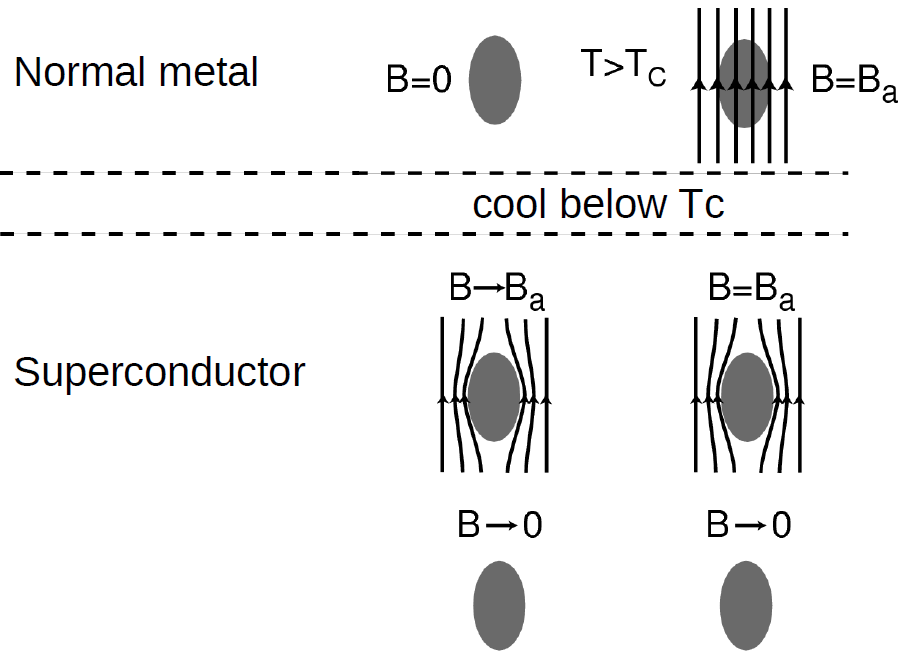
\includegraphics[width=0.8\textwidth]{immagini/Effetto_Meissner_1.png}
\end{figure}
\hspace{-0.6cm}Supponiamo che l'oggetto grigio rappresenti un materiale in grado di diventare superconduttore. Esso può trovarsi sia in assenza sia in presenza di un campo magnetico esterno.\\ Consideriamo ora la possibilità di raffreddare il sistema al di sotto della cosiddetta temperatura critica $T_c$, ossia la temperatura al di sotto della quale emerge il comportamento superconduttivo. Se inizialmente il materiale si trova a una temperatura $T > T_c$ e non è presente alcun campo magnetico, esso si comporta come un metallo normale. Raffreddando il sistema al di sotto di $T_c$, il materiale diventa superconduttore. Se a questo punto si applica un campo magnetico esterno, tale campo non riesce a penetrare all'interno del campione. Se successivamente il campo magnetico viene rimosso, all'interno del materiale non rimane alcun campo magnetico.\\
Consideriamo ora il caso opposto, in cui il materiale si trovi inizialmente nello stato normale ma in presenza di un campo magnetico applicato. In questa situazione il campo magnetico penetra all'interno del metallo, come avviene tipicamente nei conduttori normali. Tuttavia, se il materiale viene raffreddato al di sotto della temperatura critica, il campo magnetico viene espulso dal suo interno. Se successivamente il campo magnetico esterno viene spento, il sistema rimane privo di campo magnetico interno.\\
Osserviamo quindi che, indipendentemente dalle condizioni iniziali, una volta che il sistema si trova nello stato superconduttivo, cioè al di sotto della temperatura critica, il campo magnetico all'interno del materiale risulta nullo.\\
A questo punto sorge una domanda: se inizialmente abbiamo un metallo normale immerso in un campo magnetico, come è possibile che, raffreddandolo al di sotto della temperatura critica senza modificare il campo applicato, il campo magnetico all'interno del materiale diventi nullo? Questo implica che il campo magnetico totale all'interno del materiale debba essere compensato da un'altra sorgente di campo magnetico.\\
La spiegazione è la seguente. Se un materiale entra nello stato superconduttivo in presenza di un campo magnetico esterno, al momento della transizione di fase si genera una supercorrente che scorre sulla superficie del campione. Tale supercorrente produce un campo magnetico che si oppone al campo applicato e lo compensa esattamente all'interno del materiale.\\
Questo comportamento è detto diamagnetismo. Utilizzando infatti la relazione che lega il campo di induzione magnetica $\vb{B}$ al campo magnetico $\vb{H}$ e alla magnetizzazione $\vb{M}$,
\begin{equation*}
   \vb{B} = \vb{H} + 4\pi \vb{M}
\end{equation*}
si vede che, nello stato superconduttivo, la condizione $\vb{B}=0$ all'interno del materiale implica una magnetizzazione pari a
\begin{equation*}
   \vb{M} = -\frac{\vb{H}}{4\pi}
\end{equation*}
Questa relazione descrive il cosiddetto diamagnetismo perfetto, che rappresenta una delle proprietà caratteristiche dello stato superconduttivo.\\
Tipicamente, in un materiale diamagnetico, la magnetizzazione è opposta al campo magnetico esterno, ma con una suscettibilità inferiore. In questo caso, invece, si ha un comportamento diamagnetico perfetto, ed è per questo motivo che l'espulsione del campo magnetico da un superconduttore è chiamata anche effetto diamagnetico.\\
L'effetto di espulsione del campo magnetico da un superconduttore avviene solo se il campo magnetico applicato è sufficientemente piccolo. Quindi, non si verifica per qualsiasi campo magnetico applicato, ma solo se quest'ultimo è inferiore a un valore detto campo critico $H_c$. Questo campo critico dipende dalla temperatura, per cui $H_c \equiv H_c(T)$. La dipendenza del campo critico $H_c$ dalla temperatura, per molti materiali, è descritta da una legge di potenza della forma:  
\begin{equation}
   H_c(T)
   =H_c(0) \biggl[ 1 - \qty( \frac{T}{T_c} )^2 \biggr]
   \label{eq:campo_critico}
\end{equation}
dove $H_c(0)$ è il valore estrapolato del campo critico allo zero assoluto.
\begin{figure}[H]
   \centering
   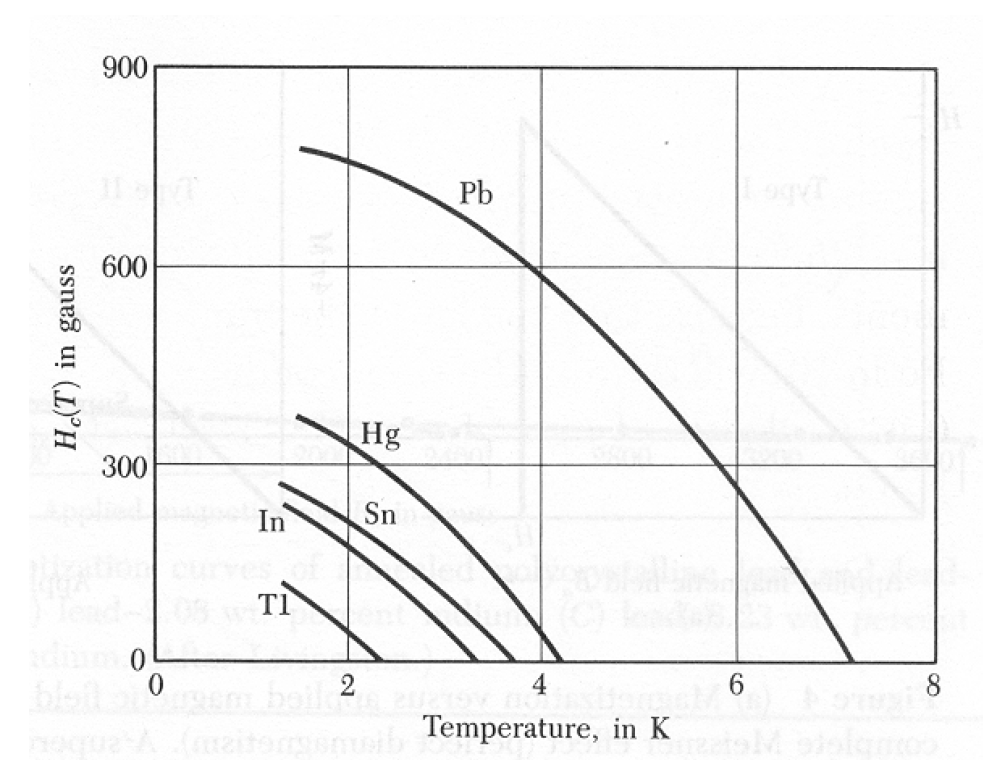
\includegraphics[width=.6\textwidth]{immagini/curve_campo_magnetico_temperatura_superconduttori.png}
   \caption*{Campo magnetico critico in funzione della temperatura per diversi materiali.}
\end{figure}
\hspace{-0.6cm}L'\eqrefcustom{eq:campo_critico} è una legge empirica. Inoltre, se sull'asse orizzontale si riporta la temperatura assoluta normalizzata rispetto alla temperatura critica, mentre sull'asse verticale si rappresenta il valore del campo magnetico esterno applicato fino al quale si osserva la superconduttività (o, equivalentemente, al di sotto del quale il materiale è superconduttivo), scalato rispetto al valore estrapolato del campo critico, tutte le curve si sovrappongono in un'unica linea che descrive accuratamente il comportamento di questa classe di materiali:
\begin{figure}[H]
   \centering
   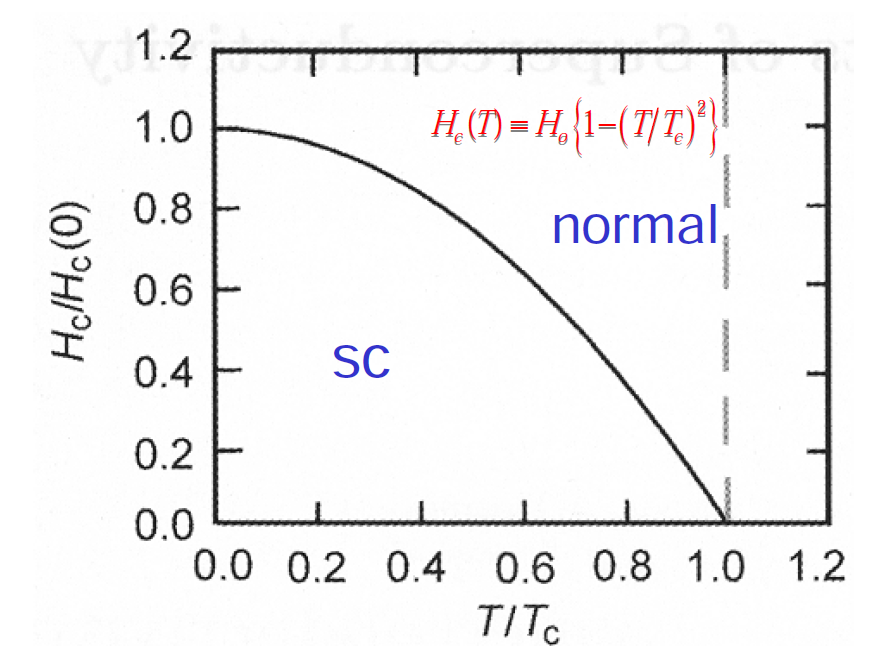
\includegraphics[width=.6\textwidth]{immagini/curve_campo_magnetico_temperatura_superconduttori_riscalate.png}
\end{figure}
\hspace{-0.6cm}Ciò che questa sorta di diagramma di fase ci dice è che nella regione dei campi magnetici inferiori a $H_c$ e delle temperature inferiori alla temperatura critica, il materiale è superconduttore. Al di sopra di questa curva, invece, il materiale si comporta come un metallo normale. Inoltre, la curva si annulla alla temperatura critica, il che significa che, per temperature superiori alla temperatura critica, indipendentemente dal valore del campo magnetico, la superconduttività non è presente.\\
Cerchiamo adesso di capire se queste due proprietà, il fatto che il materiale diventi un conduttore perfetto e il fatto che si verifichi l'espulsione del campo magnetico, rappresentino due fenomeni indipendenti oppure se una possa essere derivato dall'altro.\\
La risposta è che si tratta di due fenomeni indipendenti. Per capirne il motivo, supponiamo che un superconduttore sia semplicemente un conduttore perfetto (ossia supponiamo che il materiale abbia resistenza nulla in determinate condizioni, che è ciò che intendiamo con questa definizione) e cerchiamo di capire quale sarebbe la sua risposta a un campo magnetico applicato. Confrontiamo poi questa risposta con quella effettivamente osservata in un superconduttore.\\
Supponiamo quindi di avere un conduttore perfetto, descritto come un materiale con resistività nulla. Dalla legge di Ohm sappiamo che il campo elettrico è dato da:
\begin{equation*}
   \vb{E}=\rho\vb{J}
\end{equation*}
Dunque, se la resistività $\rho$ è zero, significa che in un conduttore perfetto il campo elettrico è nullo, anche in presenza di una corrente non nulla.\\
Se ora utilizziamo la legge di Faraday, sappiamo che il rotore del campo elettrico è legato alla derivata temporale del campo magnetico da:
\begin{equation*}
   \curl{\vb{E}}=-\frac{1}{c} \pdv{\vb{B}}{t}
\end{equation*}
Dato che in un conduttore perfetto il campo elettrico è nullo, ciò implica che il campo magnetico deve rimanere costante nel tempo. Quindi per un conduttore perfetto ci aspettiamo che possano esserci correnti non nulle, resistività nulla, ma che il campo magnetico rimanga costante nel tempo.\\
Proviamo ora a prevedere cosa osserveremmo in un conduttore perfetto considerando due situazioni:
\begin{enumerate}[leftmargin=0.7cm, label=(\alph*)]
   \item Un conduttore perfetto in assenza di campo magnetico, che viene raffreddato sotto la temperatura critica.
   \item Un conduttore perfetto in presenza di un campo magnetico applicato, che viene raffreddato sotto la temperatura critica.
\end{enumerate}
Confronteremo poi queste previsioni con il comportamento reale di un superconduttore.
\begin{figure}[H]
   \centering
   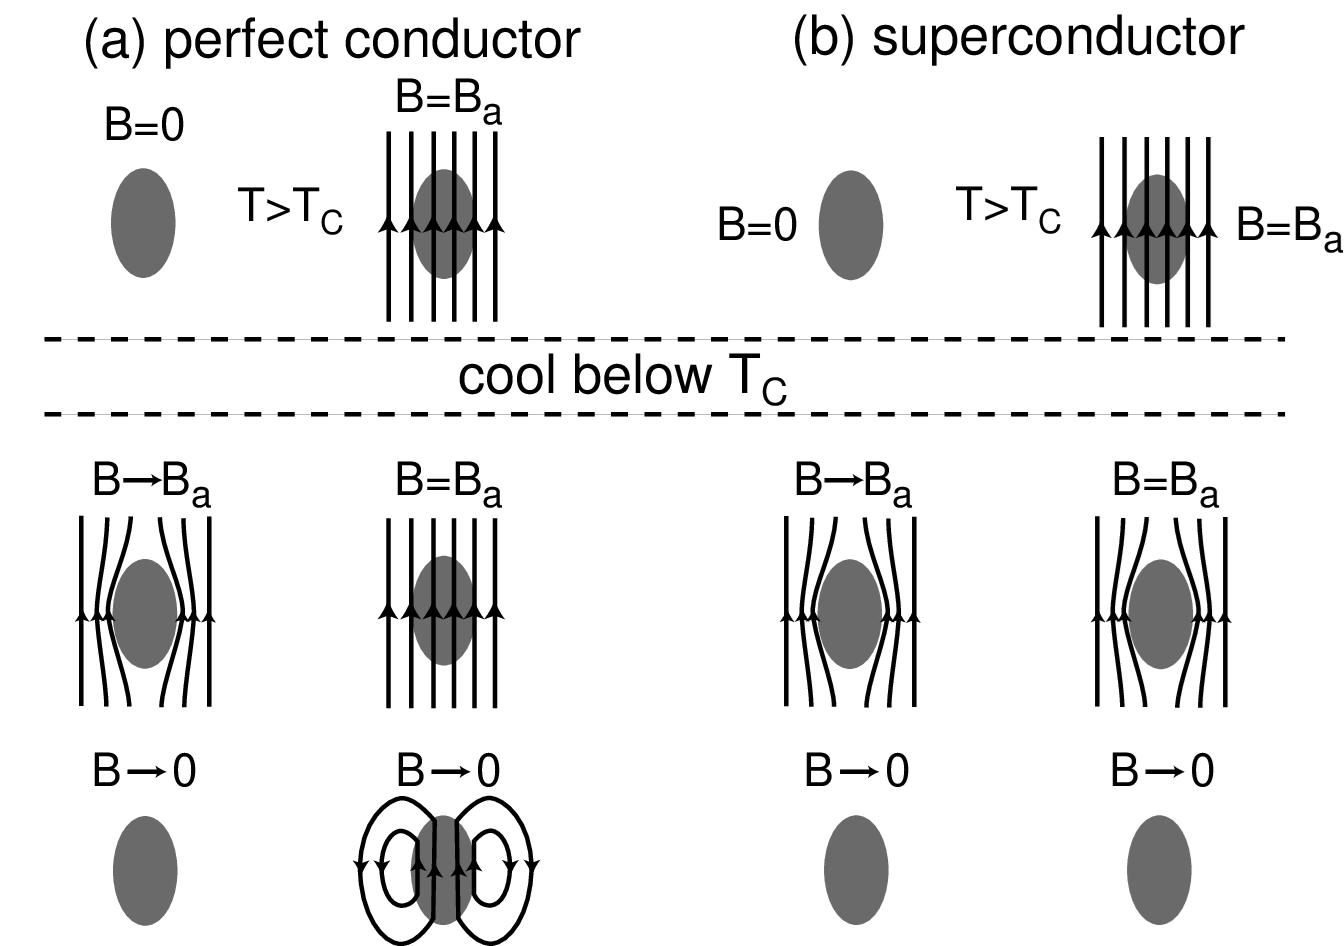
\includegraphics[width=.9\textwidth]{immagini/confronto_conduttori_perfetti_superconduttori.png}
\end{figure}
\hspace{-0.6cm}Iniziamo dall'esperimento sulla sinistra. Se inizialmente non abbiamo un campo magnetico applicato, ci aspettiamo che raffreddando il materiale, poiché $\vb{B}$ deve rimanere costante, dato che inizialmente era nullo all'interno del materiale esso sarà ancora pari a zero anche quando il materiale sarà diventato superconduttore e resterebbe nullo anche se accendessimo e poi spegnessimo un campo magnetico. Questo tipo di comportamento sarebbe perfettamente spiegato dalla teoria del conduttore perfetto.\\
Vediamo ora cosa accade se invece consideriamo un conduttore perfetto in presenza di un campo magnetico applicato. All'inizio, essendo un metallo normale, il campo magnetico penetra nel materiale. Supponiamo ora di raffreddarlo: se il materiale è un conduttore perfetto, la legge di Faraday ci dice che $\vb{B}$ dovrebbe rimanere costante nel tempo, quindi il campo magnetico dovrebbe rimanere all'interno del materiale. Anche se spegniamo il campo esterno, il campo magnetico dovrebbe persistere all'interno del conduttore perfetto. Tuttavia, questo non è ciò che si osserva in un superconduttore, in quanto quando un materiale diventa superconduttore in presenza di un campo magnetico applicato il campo viene espulso dal materiale. Se confrontiamo i due casi, conduttore perfetto in presenza di un campo magnetico e superconduttore in presenza di un campo magnetico, vediamo una differenza fondamentale.\\
Tale fatto ci dice che la conducibilità perfetta (cioè resistività nulla) non è sufficiente per spiegare il comportamento osservato nei superconduttori quando il campo magnetico iniziale è diverso da zero. In particolare, l'effetto Meissner non può essere spiegato solo con la perfetta conducibilità. Queste considerazioni ci portano a concludere che la perfetta conducibilità e il perfetto diamagnetismo sono due fenomeni indipendenti.
%Let's start from the left experiment, We have zero applied magnetic field, we cool down the material then what we have to expect in this case that B is constant so zero initially zero when there is an applied magnetic field even below the critical temperature and still zero if we turn off the field. This type of experiment would be perfectly explained for a perfect conductor.\\
%Let's see what happens if instead we describe what we would expect for a perfect conductor if initially there is an applied magnetic field. So in a perfect conductor in an applied magnetic field, since it's a normal metal, there is an applied field that penetrates the conductor. Now let's suppose we cool it down but if we cool it down since $\vb{B}$ should stay constant we have to expect that the magnetic field still persists inside the material and if we switch off the applied magnetic field still this magnetic field should exist inside the perfect conductor. So for a perfect conductor in an applied magnetic field even if we force it to undergo a transition below the critical temperature we should expect that the magnetic field still remains inside the material. But this is not what we observe for a superconductor because what we observe for a superconductor in the presence of an applied magnetic field when we induce the transition in the presence of an applied magnetic field is the expulsion of the magnetic field out of the material. So if we compare these two left, these two columns, this one what happens in an applied magnetic field for a perfect conductor and what happens in an applied magnetic field for a superconductor we see a difference. This tells us that perfect conductivity, meaning zero resistivity, cannot explain what happens to a superconductor when the magnetic field is different from zero initially, whereas it would explain what happens if there is no applied magnetic field. So the peculiar Meissner effect which is the expulsion of the magnetic field out of the sample cannot be explained by the perfect conductivity. So this tells us that these two phenomena, perfect conductivity and perfect diamagnetism, are two independent phenomena. In summary, perfect conductivity cannot explain the Meissner effect.
\subsection{Termodinamica della transizione N--SC}
%Let's try to rephrase what we have observed. The superconductor is characterized by the condition $B=0$ inside it independently on how the system has reached this condition, so there is zero magnetic field inside if there was not inside at the beginning then the magnetic field was turned on and then it is turned off and there is zero magnetic field inside even if we initially had the magnetic field inside. In other words, in the superconducting phase we have the same state with zero magnetic field inside independently on how the system has reached this condition. This means that the superconducting phase is a thermodynamically stable phase of the material, and this leads us to describe it in thermodynamic terms. In particular, ew can describe the two conditions of the material, which is either normal or superconducting, as different phases of matter which we have to describe in terms of appropriate thermodynamic potential.
Proviamo a riformulare ciò che abbiamo osservato. Il superconduttore è caratterizzato dalla condizione $\vb{B}=0$ al suo interno, indipendentemente da come il sistema abbia raggiunto questa condizione. Ciò significa che il campo magnetico all'interno è nullo sia nel caso in cui inizialmente non fosse presente, poi acceso e successivamente spento, sia nel caso in cui inizialmente fosse presente. In altre parole, nella fase superconduttiva si ha sempre lo stesso stato con campo magnetico nullo all'interno, indipendentemente dal modo in cui il sistema ha raggiunto questa condizione. Questo implica che la fase superconduttiva è una fase termodinamicamente stabile del materiale, il che ci porta a descriverla in termini termodinamici. In particolare, possiamo descrivere le due condizioni del materiale, ovvero lo stato normale e quello superconduttivo, come fasi distinte della materia, che dobbiamo rappresentare attraverso un opportuno potenziale termodinamico.\\
%The idea is that the system reaches the thermodynamic stable state following the second law of thermodynamics, provided we use the appropriate thermodynamic potential. Describing a system using the appropriate thermodynamic potential means identifying the thermodynamic potential which stays constant at the transition, where the transition takes place in particular changing the temperature and changing the applied magnetic field, so we have to find the appropriate thermodynamic potential which is stable at the transition when the two variables which change, we modify, are magnetic field and temperature. Then let's make a step in between and remind which are the thermodynamic relations in the presence of a magnetic field in general and this will lead us to identify which is the appropriate thermodynamic potential to describe the superconductive transition. First of all we have to identify what is the system. The system is a magnetized sample of the material of fixed volume $V$ and magnetic field. Let's write the two most common free energies for this system, which are the Helmholtz free energy and the Gibbs free energy and now we are going to see how to write these two free energies.
L'idea è che il sistema raggiunga lo stato termodinamicamente stabile seguendo la seconda legge della termodinamica\mn{Tale principio afferma che "Per un sistema chiuso, l'entropia $S$ aumenta, mentre $U$, $H$, $F$ e $G$ diminuiscono, nei limiti consentiti dalla termodinamica. Ciò permette di formulare affermazioni sulla stabilità degli stati di equilibrio termodinamico.".}, a condizione che si utilizzi il potenziale termodinamico appropriato. Descrivere un sistema attraverso il potenziale termodinamico appropriato significa identificare il potenziale termodinamico che rimane costante durante la transizione, la quale avviene in particolare al variare della temperatura e del campo magnetico applicato. Dobbiamo quindi trovare il potenziale termodinamico adeguato, che sia stabile durante la transizione quando le due variabili che modifichiamo, ovvero il campo magnetico e la temperatura, cambiano.\\
Facciamo ora un passo intermedio e ricordiamo quali sono le relazioni termodinamiche in presenza di un campo magnetico in generale: questo ci porterà a identificare il potenziale termodinamico più adatto a descrivere la transizione superconduttiva. Per prima cosa, dobbiamo identificare il sistema. Il sistema è un campione magnetizzato del materiale di volume fissato $V$ e con campo magnetico definito. Scriviamo quindi le due energie libere più comuni per questo sistema, ovvero l'energia libera di Helmholtz e l'energia libera di Gibbs, e vediamo ora come esprimerle:
\begin{itemize}[leftmargin=0.5cm]
   \item L'energia libera di Helmholtz $F$ è definita come:
   \begin{equation*}
      F=E - TS
   \end{equation*}
   dove $E$ è l'energia interna del sistema e $S$ è l'entropia. Se facciamo una variazione infinitesima di queste quantità, avremo una variazione infinitesima dell'energia libera, data da:
   \begin{equation*}
      \dd{F}
      =\dd{E} - \dd{(TS)}
      =\dd{E} - T\dd{S} - S\dd{T}
   \end{equation*}
   Dalla prima legge della termodinamica sappiamo che $\dd{E}=\var{Q} - \dd{W}$, dove $-\dd{W}$ è il lavoro magnetico svolto sul sistema per stabilire il campo nel volume $V$ e magnetizzare il campione. Inoltre, in una trasformazione quasi-statica e reversibile, il calore scambiato si scrive come: $\var{Q}=T\dd{S}$, per cui possiamo scrivere
   \begin{equation*}
      \dd{F}
      =( T\dd{S} - \dd{W} ) - T\dd{S} - S\dd{T}
      =- \dd{W} - S\dd{T}
   \end{equation*}
   Il lavoro magnetico può essere espresso in termini del differenziale dell'energia del campo magnetico:
\begin{equation*}
   \dd{W}
   =\dd{ \qty( \frac{V H^2}{8\pi} ) } + V H \dd{M}
\end{equation*}
dove il primo termine è dato dal prodotto del volume del materiale moltiplicato per la densità di energia del campo magnetico e il secondo termine è l'energia necessaria per magnetizzare il campione. Poiché $V$ è costante, possiamo scrivere:
\begin{equation*}
   \dd{ \qty( \frac{V H^2}{8\pi} ) }
   =\frac{V H}{4\pi} \dd{H}
\end{equation*}
e quindi, ricordando che $B=H + 4\pi M$, otteniamo:
\begin{equation*}
   \dd{W}
   =\frac{V H}{4\pi} ( \dd{H} + 4\pi \dd{M} )
   =\frac{V}{4\pi} H \dd{B}
\end{equation*}
Di conseguenza, la variazione dell'energia libera di Helmholtz è data da
\begin{equation*}
   \dd{F(T,B)}
   =- \frac{V}{4\pi} H \dd{B} - S \dd{T}
\end{equation*}
Dall'espressione della variazione infinitesima dell'energia libera di Helmholtz, vediamo che esso è il potenziale termodinamico appropriato quando consideriamo una transizione che implica una temperatura $T$ e un'induzione magnetica $B$ costanti.
\item Se invece consideriamo l'energia libera di Gibbs, che per un sistema magnetico è definita come
\begin{equation}
   G(T,H)=F(T,B) - \frac{V}{4\pi} H B
   \label{eq:relazione_G_F}
\end{equation}
e ne facciamo una variazione infinitesima, otteniamo\mn{Nel caso più generale si ha che
\begin{equation*}
   \dd{(HB)}=\dd{H}B + H\dd{B}
\end{equation*}
ma essendo in questo caso $H$ costante, si ha che $\dd{(HB)}=H\dd{B}$.}:
\begin{equation*}
   \dd{G(T,H)}
   = - S \dd{T} - \frac{V}{4\pi} B \dd{H}
\end{equation*}
Ciò significa che $G$ è il potenziale termodinamico appropriato per una transizione che avviene a temperatura e campo magnetico $H$ fissati. Infatti, come abbiamo detto, quando avviene la transizione superconduttiva, il campo magnetico $\vb{B}$ viene espulso dal superconduttore. Questo significa che, per descrivere termodinamicamente la fase superconduttiva, non abbiamo bisogno di un potenziale termodinamico che dipenda dalle variazioni di $B$, ma piuttosto di un potenziale termodinamico che sia legato alle variazioni del campo magnetico esterno applicato, $H$. Questo $H$ viene mantenuto costante, poiché generalmente rappresenta il campo prodotto da una sorgente esterna, e non il campo magnetico presente nel campione.
\end{itemize}
%In fact, as we said when the superconductor transition takes place the magnetic field $\vb{B}$ is expelled from the superconductor, so it means that in order to describe thermodynamically the superconducting phase we do not need a thermodynamic potential which depends on variations of $B$ but we need a thermodynamic potential which is related to variations of the externally applied magnetic field $H$. This $H$ we keep constant because typically it is the field which comes from an externally applied field and not the magnetic field present in the sample.
Cerchiamo adesso di avvicinarci un po' di più a ciò che accade durante la transizione dalla fase normale alla fase superconduttiva in una geometria molto semplice. Supponiamo di avere un metallo di forma cilindrica di raggio $r_0$ e lunghezza $L$ posto all'interno di un solenoide di raggio $R$, lunghezza $L$ e avente $N$ spire.
\begin{figure}[H]
   \centering
   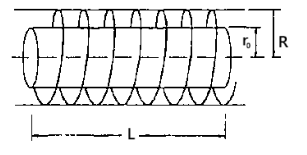
\includegraphics[width=.65\textwidth]{immagini/Cilindro_superconduttore.png}
\end{figure}
\hspace{-0.6cm}Partiamo dall'energia libera di Helmholtz e scriviamola per le due fasi, normale e superconduttiva. Nella fase normale abbiamo:
\begin{equation*}
   F_n=
   V f_{n,0} + V \frac{H_a^2}{8\pi} + V_{\text{ext}} \frac{H_a^2}{8\pi}
\end{equation*}
dove il primo termine rappresenta il contributo dell'energia libera di Helmholtz per unità di volume del campione nella fase normale in assenza di campo magnetico applicato, indicato con $f_{n,0}$, moltiplicato per il volume $V$ del materiale,\sn{Tale contributo è intrinseco alla fase normale del materiale e avrà un'espressione analoga quando il materiale sarà superconduttore.} mentre gli altri due termini rappresentano i contributi, se $H_a$ è il campo magnetico applicato proveniente dalla corrente che scorre nel solenoide, dovuti alla presenza di un campo magnetico all'interno del materiale e alla presenza di un campo magnetico nella parte del volume che si trova all'interno del solenoide, ma esterna al materiale (quindi $V_{\rm ext}$ rappresenta essenzialmente il volume di questa regione).\\  
%Now let's try to go a bit closer to what happens in the transition from the normal phase to the superconducting phase in a very simple geometry. Let's suppose we have a metal with a cylindrical shape and it is inside a solenoid of $N$ coils. Let's start from the Helmholtz free energy and we write it for the two phases, normal and superconducting. So in the normal phase we have where the first term is the contribution of the Helmholtz free energy per unit volume of the sample in the normal phase at zero applied magnetic field $f_n$ times the volume $V$ of the material\mn{Notice that this contribution is something which is intrinsic of the normal phase of the material. We will have the analogous expression when the material is superconducting}, and the other two terms are the contributions, if $H_a$ is the applied magnetic field coming from the current flowing in the solenoid, related to having a magnetic field inside the material plus the magnetic field in the part of the volume which is inside the solenoid, but external to the material (so $V_{\rm ext}$ is basically the volume of the region outside the material).\\
Nella fase superconduttiva, poiché abbiamo detto che non c'è campo magnetico applicato all'interno, non abbiamo il secondo contributo e quindi l'energia libera di Helmholtz è data da
\begin{equation*}
   F_s=
   V f_{s,0} + V_{\text{ext}} \frac{H_a^2}{8\pi}
\end{equation*}
Consideriamo adesso la differenza tra le due energie:
\begin{equation}
   F_n - F_s
   =V ( f_{n,0} - f_{s,0} ) + V \frac{H_a^2}{8\pi}
   \label{eq:differenza_energie_libere}
\end{equation}
\mn{Questa parte è da sistemare, chiedere ad Adriano o alla prof.}Supponiamo che il materiale sia inizialmente nella fase normale e che poi la temperatura venga modificata fino a farlo diventare superconduttore, mantenendo fissa la corrente nel solenoide (in quanto supponiamo che esso sia collegato ad un generatore) e quindi il campo magnetico applicato. In questo caso, poiché all'interno del materiale si verifica un cambiamento del campo magnetico (in quanto il campo viene espulso dal superconduttore), ci sarà una variazione del flusso del campo magnetico attraverso qualsiasi superficie avente come contorno il solenoide. Questo implica, per la legge di Faraday, che esiste un'energia associata a questo processo, data da:
%Suppose that this material is initially in the normal phase and then we change the temperature until it becomes superconducting while keeping fixed the current in the solenoid and so the magnetic field. Then, since what happens inside the material is a change of the magnetic field (because the magnetic field is expelled inside the material) we will have a variation of the flux of the magnetic field through any surface which has a solenoid as a contour. This implies, from the Faraday's law, that there is an energy related to this process which is given by
\begin{equation*}
   \dd{W}=\mathcal{E} I \dd{t}
\end{equation*}
dove $\mathcal{E}$ è la forza elettromotrice indotta e $I$ è la corrente che scorre nel solenoide. Se il processo avviene per un tempo finito, l'energia totale sarà data dall'integrale:
\begin{equation*}
   W=\int_{0}^{T} \mathcal{E} I \dd{t}
\end{equation*}
Dalla legge di Faraday sappiamo che $\mathcal{E}$ è data da
\begin{equation*}
   \mathcal{E}
   =-\frac{N}{c} \dv{\Phi}{t}
\end{equation*}
e sostituendo nell'integrale otteniamo\mn{Il flusso attraverso la superficie di una spira nella fase normale è dato da
\begin{equation*}
   \Phi_n=H_a \pi R^2
\end{equation*}
mentre nella fase superconduttiva è dato da
\begin{equation*}
   \Phi_s=H_a \pi \qty( R^2 - r_0^2 )
\end{equation*}
in quanto non si ha contributo dalla parte occupata dal materiale in fase superconduttiva.}:
\begin{equation*}
   W
   =-\int_{0}^{T} \frac{N}{c} \dv{\Phi}{t} I \dd{t}
   =-\int_{\Phi_n}^{\Phi_s} \frac{N I}{c} \dd{\Phi}
   =\frac{N I}{c} ( \Phi_n - \Phi_s )
   =\frac{N I}{c} \pi r_0^2 H_a
\end{equation*}
Inoltre, per il teorema della circuitazione di Ampere il campo magnetico $H_a$ all'interno del solenoide soddisfa la relazione
\begin{equation*}
   H_a L
   =\frac{4\pi}{c} N I
\end{equation*}
che invertita ci permette di scrivere
\begin{equation}
   W
   =\frac{H_a L}{4\pi} \pi r_0^2 H_a
   =V \frac{H_a^2}{4\pi}
   \label{eq:energia_associata}
\end{equation}
dove $V=4 \pi r_0 L$ è il volume del cilindro di materiale.\\
Mettiamo adesso in relazione la differenza tra le due energie libere con l'energia fornita dalla sorgente esterna della corrente. Infatti, la differenza nell'energia libera di Helmholtz è un'energia che entra nel sistema, proveniente originariamente dal generatore che fornisce la corrente che scorre nel circuito. Confrontando l'\eqrefcustom{eq:differenza_energie_libere} con l'\eqrefcustom{eq:energia_associata} otteniamo che
\begin{equation*}
   V ( f_{n,0} - f_{s,0} ) + V \frac{H_a^2}{8\pi}
   =V \frac{H_a^2}{4\pi}
\end{equation*}
cioè
\begin{equation*}
   f_{n,0} - f_{s,0}
   =\frac{H_a^2}{8\pi}
\end{equation*}
In questo modo ci rendiamo conto che l'energia libera di Helmholtz per unità di volume è legata al campo magnetico applicato. Tuttavia, si verifica una differenza quando avviene la transizione di fase, che si manifesta non per un campo magnetico qualsiasi, ma quando il campo applicato è il campo critico $H_c$. Quindi, alla transizione di fase, otteniamo la seguente espressione, sostituendo $H$ con il campo critico:
\begin{equation}
   f_{n,0} - f_{s,0} = \frac{H_c^2(T)}{8\pi}
   \label{eq:relazione_termodinamica_campo_critico}
\end{equation}
In questo modo otteniamo la cosiddetta definizione termodinamica del campo critico, poiché stabilisce una relazione tra una grandezza termodinamica (la densità di energia libera) e una grandezza elettrodinamica (la densità di energia del campo magnetico), ma sotto la condizione specifica di avere il campo critico, ovvero nel punto in cui avviene la transizione. Utilizzeremo questa relazione quando descriveremo la transizione di fase in termini termodinamici, in particolare nel contesto della teoria di Ginzburg--Landau.\\
Abbiamo detto in precedenza che il potenziale termodinamico corretto per descrivere la transizione non è l'energia libera di Helmholtz, ma l'energia libera di Gibbs. Esplicitiamo allora la differenza di energia libera di Gibbs tra la fase normale e quella superconduttiva: per farlo, utilizziamo semplicemente la definizione che collega l'energia libera di Gibbs all'energia libera di Helmholtz, data dall'\eqrefcustom{eq:relazione_G_F}. Si ha
\begin{equation*}
   \begin{split}
      G_n(T,H) - G_s(T,H)
      & =F_n(T,B) - F_s(T,B) - V\frac{H_a^2}{4\pi}
      \\
      & =V ( f_{n,0} - f_{s,0} ) + V \frac{H_a^2}{8\pi} - V\frac{H_a^2}{4\pi}
      \\
      & =\frac{V}{8\pi} \bigl[ H_c^2(T) - H_a^2 \bigr]
   \end{split}
\end{equation*}
dove nel secondo passaggio abbiamo usato l'\eqrefcustom{eq:differenza_energie_libere} e nel terzo l'\eqrefcustom{eq:relazione_termodinamica_campo_critico}.\\
In definitiva abbiamo trovato che
\begin{equation}
   G_n(T,H) - G_s(T,H)
   =\frac{V}{8\pi} \bigl[ H_c^2(T) - H_a^2 \bigr]
   \label{eq:differenza_Gibbs}
\end{equation}
Il risultato ottenuto mostra che la differenza tra le energie libere di Gibbs è espressa in termini della differenza tra il quadrato del campo critico e il quadrato del campo applicato. Questo ci dice che:
\begin{itemize}[leftmargin=0.5cm]
   \item Se il campo applicato è maggiore del campo critico, questa quantità è negativa, il che implica che l'energia libera di Gibbs nella fase normale è minore di quella nella fase superconduttiva. Di conseguenza, la fase stabile (cioè quella con il minimo potenziale termodinamico) è la fase normale. Quindi, per un campo applicato superiore al campo critico, la fase normale è la fase stabile.
   \item Se invece il campo applicato è minore del campo critico, questa quantità è positiva, il che significa che l'energia libera di Gibbs nella fase normale è maggiore di quella nella fase superconduttiva. In questo caso, la fase stabile è la fase superconduttiva.
   \item Infine, se il campo applicato è esattamente uguale al campo critico, le due fasi hanno la stessa energia libera di Gibbs. Questo è precisamente ciò che accade alla transizione di fase, in cui l'energia libera di Gibbs, il potenziale termodinamico rilevante per entrambe le fasi, assume lo stesso valore.
\end{itemize}
%In this way we realize that the Helmholtz free energy per unit volume is related to the applied magnetic field. But we have this difference if we have the phase transition, which happens if the applied field is not any generic magnetic field, but it is the critical field $H_c$. So at the phase transition we obtain the expression here, but with $H$ replaced by the critical magnetic field:
%In this way we obtain what is called the thermodynamic definition of the critical field, because we have a relation between a thermodynamic quantity, which is a free energy density, and an electro-dynamic quantity, which is a energy density of a magnetic field, but under the specific condition of having the critical field, so when the transition takes place. We will use this relation whenever we will describe the phase transition in thermodynamic terms, and this is in particular what we do with Ginzburg--Landau theory.\\
%We said previously that the proper thermodynamic potential for describing the transition is not the Helmholtz free energy, but the Gibbs free energy, so what we do now is to write explicitly the Gibbs free energy difference in the normal and in the superconducting phase and to do that we just use the definition, which relates to the Gibbs free energy with the Helmholtz free energy, which is given by \eqrefcustom{eq:relazione_G_F}.
%So the result is that the difference in the Gibbs free energies is expressed in terms of the difference between the critical field squared minus the applied field squared. This tells us that, if the applied field is larger than the critical field, this quantity is negative, so this means that the Gibbs free energy in the normal phase is smaller than the Gibbs free energy in the superconducting phase. This means that the stable phase, which is the one which has the minimum thermodynamic potential, is the normal phase. So if we have a field larger than the critical field, the stable phase is the normal phase. If instead the applied field is smaller than the critical field, this quantity is positive, so it means that the Gibbs free energy in the normal phase is larger than the Gibbs free energy in the superconducting phase, so the stable phase is the superconducting. If instead the applied field is equal to the critical field, the two phases have the same Gibbs free energy, which is exactly what happens at the phase transition where the Gibbs free energy, the relevant thermodynamic potential for the two phases, have the same value.
%So in this way, in this simple example where we can perform all the calculations to derive the Gibbs free energies, we can really see which is the stable phase when we change the externally applied magnetic field for a system which undergoes a phase transition with expulsion of the magnetic field out of the material, because the only assumption we have done here is that in the free energies we do not have any term coming from the magnetic field in the material, which is the characteristic of the Meissner effect.\\
%From the thermodynamic potential we can derive thermodynamic properties of the material, in particular the specific heat and the entropy. So what we do is use again thermodynamics to write the entropy difference between the two phases, which is given by the opposite of the derivative of the Gibbs free energy with respect to temperature at fixed applied field.
Attraverso questo semplice esempio in cui possiamo eseguire facilmente tutti i calcoli per derivare le energie libere di Gibbs, possiamo vedere chiaramente quale sia la fase stabile al variare del campo magnetico applicato esternamente, per un sistema che subisce una transizione di fase con espulsione del campo magnetico dal materiale. Ciò è possibile perché l'unica assunzione che abbiamo fatto è che nelle energie libere non sia presente alcun termine dovuto al campo magnetico all'interno del materiale, che è proprio la caratteristica dell'effetto Meissner.\\
Dal potenziale termodinamico possiamo poi ricavare le proprietà termodinamiche del materiale, in particolare il calore specifico e l'entropia. Ciò che facciamo ora è sfruttare nuovamente la termodinamica per scrivere la differenza di entropia tra le due fasi, che è data dall'opposto della derivata dell'energia libera di Gibbs rispetto alla temperatura, mantenendo fisso il campo applicato. Dunque:
\begin{equation}
   S_s - S_n
   =\biggl. \pdv{G_n}{T} \biggr|_H - \biggl. \pdv{G_s}{T} \biggr|_H
   =\frac{V}{4\pi} H_c \dv{H_c}{T}
   \label{eq:differenza_entropie}
\end{equation}
La dipendenza del campo critico dalla temperatura è data dall'\eqrefcustom{eq:campo_critico}, la quale ci dice che la sua derivata è minore di zero. Questo fatto rappresenta un altro modo per esprimere che la fase superconduttiva ha un'entropia inferiore rispetto alla fase normale, a condizione che il campo sia minore del campo critico nell'intervallo di temperatura considerato.\\
Dalla conoscenza dell'entropia possiamo calcolare il calore specifico semplicemente derivando l'entropia rispetto alla temperatura e moltiplicando per la temperatura. Valutando la differenza otteniamo:
\begin{equation*}
   C_s - C_n = T \biggl. \pdv{S_s}{T} \biggr|_H - \biggl. T \pdv{S_n}{T} \biggr|_H
   =\frac{V}{4\pi} T \qty[ \qty( \dv{H_c}{T} )^2 + H_c \dv[2]{H_c}{T} ]
\end{equation*}
Da questa espressione possiamo analizzare la variazione del calore specifico tra la fase normale e la fase superconduttiva in due condizioni: quando la transizione avviene in assenza di campo applicato e quando avviene con un campo applicato finito, poiché il peso dei due contributi dipende dal campo critico.\\
Studiamo il calore specifico perché la sua variazione ci permette di determinare il tipo di transizione di fase. In particolare, per $H_c=0$, il secondo termine della formula si annulla e rimane solo il primo, che è sempre positivo. Ciò implica che il calore specifico è sempre positivo. Inoltre, il calore latente è nullo, perché è definito come:
\begin{equation*}
   L = T(S_n - S_s)
\end{equation*}
e, dall'\eqrefcustom{eq:differenza_entropie}, per $H_c=0$ risulta $L = 0$. Ciò significa che, in assenza di campo magnetico applicato, il calore specifico presenta una discontinuità e il calore latente è nullo. Di conseguenza, la transizione di fase a $H = 0$ è del secondo ordine.\\
Se invece consideriamo il caso in cui sia presente un campo applicato, la transizione avviene a una temperatura $T$ inferiore alla temperatura critica $T_c$ se il campo è più basso. In queste condizioni, il calore latente è dato da:
\begin{equation*}
   L = T \frac{V}{4\pi} H_c \dv{H_c}{T}
\end{equation*}
e risulta negativo. Questo significa che, in presenza di un campo applicato, la transizione di fase è del primo ordine.\\
Quanto detto si può osservare anche analizzando il comportamento del calore specifico in funzione della temperatura:
%which tells us that its derivative is smaller than zero. This fact represents another way of saying that the superconductive phase has a lower entropy than the normal phase provided the field is smaller than $H_c$ in this temperature range.\\
%From the knowledge of the entropy, we can evaluate the specific heat just performing the derivative with respect to temperature of the entropy and multiplying by the temperature. Evaluating the difference we find
%\begin{equation*}
%   C_s - C_n
%   =T \biggl. \pdv{S_s}{T} \biggr|_H - \biggl. T \pdv{S_n}{T} \biggr|_H
%   =\frac{V}{4\pi} T \qty[ \qty( \dv{H_c}{T} )^2 + H_c \dv[2]{H_c}{T} ]
%\end{equation*}
%From this expression we can see what's the specific heat variation between the normal and the superconducting phase in two conditions: when we consider the transition at zero applied field and when we consider the transition at a finite applied field, because the weight of the two contributions depends on the critical field.\\
%The reason why we study the specific heat is because depending on how the specific heat changes, we can identify which type of phase transition we have. In particular, for zero applied field the second term vanishes and remains only the first one, which is always positive. This implies that the specific heat is always positive. In addition we have a zero latent heat, because it is defined as
%\begin{equation*}
%   L
%   =T(S_n - S_s)
%\end{equation*}
%so it follows from \eqrefcustom{eq:differenza_entropie} that for $H_c=0$ we have $L=0$. So it means that at zero magnetic field we have a discontinuity in the specific heat, because as we see the difference is non vanishing and zero latent heat. So it means that at zero applied magnetic field we have a second order phase transition.\\ If we instead consider the case where we have an applied field, the transition takes place at a temperature $T$ smaller than the critical temperature $T_c$ if the field is smaller, so it means that the latent heat, which under these conditions is expressed by
%\begin{equation*}
%   L
%   =T \frac{V}{4\pi} H_x \dv{H_c}{T}
%\end{equation*}
%is negative. This means that under this condition we will have a first order phase transition. And this we can also see if we look at the behavior of the specific heat as a function of temperature:
\begin{figure}[H]
   \centering
   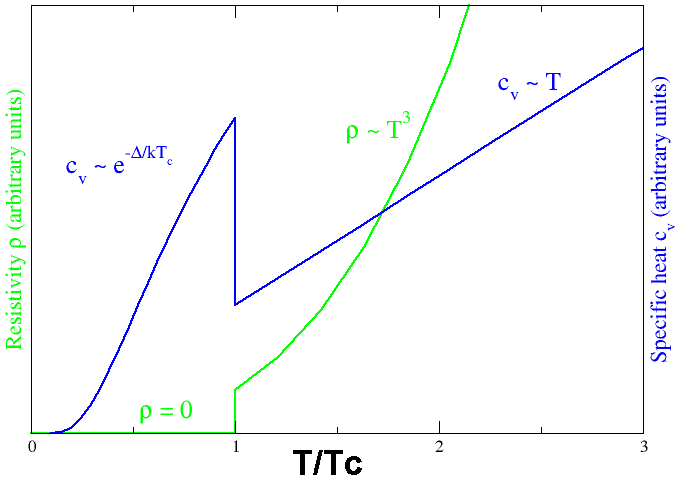
\includegraphics[width=0.65\textwidth]{immagini/andamento_calore_specifico_in_funzione_della_temperatura.png}
   \caption*{Andamento del calore specifico (in blu) e della resistività (in verde) per un superconduttore in funzione della temperatura.}
\end{figure}
\hspace{-0.6cm}Osserviamo che sopra la temperatura critica, il comportamento è quello tipico dei sistemi metallici, con una dipendenza lineare della capacità termica dalla temperatura. Tuttavia, alla temperatura critica, si verifica una discontinuità nel calore specifico, seguita, a temperature inferiori, da un comportamento completamente diverso. In particolare, a basse temperature, il calore specifico segue una dipendenza di tipo esponenziale, il che suggerisce l'emergere di una nuova scala energetica nel sistema, fatto che vediamo chiaramente nella forma $\exp(-\text{energia}/k_B T_c)$. La presenza di questa dipendenza esponenziale indica che entra in gioco una nuova scala di energia, che chiamiamo $\Delta$. Scopriremo che essa rappresenta una misura della gap energetica nello spettro di un superconduttore. Infatti, nello spettro energetico di un superconduttore, esiste un intervallo di energia proibito per le eccitazioni.\\
Il concetto di gap energetico è analogo a quello dei semiconduttori, ma il meccanismo fisico che lo genera è completamente diverso.
%We see that above the critical temperature we have a behavior which is typical of the metallic systems, so linear in temperature, we have a discontinuity of the specific heat at the critical temperature and then for lower temperatures we have a completely different temperature dependence on the specific heat which is, and this is true particularly for small temperatures, an exponential type, and is an indicative of a new energy scale coming into place, because we have a dependence in the form of the exponential to the minus some energy divided by $k_BT_c$. The fact that we have this type of exponential behavior which describes this dependence indicates that there is some new energy scale coming into play. This energy scale is what we call $\Delta$, which we are going to see is a measure of the gap we have in the energy spectrum of a superconductor. In fact, we are going to see that in the spectrum of a superconductor we have an energy regime for excitations of the superconductor which is forbidden. The concept of energy gap in the energy spectrum is analogous to what we have in a semiconductor, but the process is totally different.\\
In questo grafico vediamo anche a sinistra il comportamento della resistività in un superconduttore. Osserviamo che è zero per temperature inferiori alla temperatura critica, mentre per temperature superiori la resistività segue il comportamento tipico dei sistemi elettronici, con una dipendenza dalla temperatura di $T^3$.
\subsection{Gap nello spettro di eccitazione}
Come abbiamo detto, il comportamento esponenziale del calore specifico indica la presenza di un gap nello spettro, il che significa che la densità degli stati all'energia di Fermi presenta un intervallo di energie proibite:
\begin{figure}[H]
   \centering
   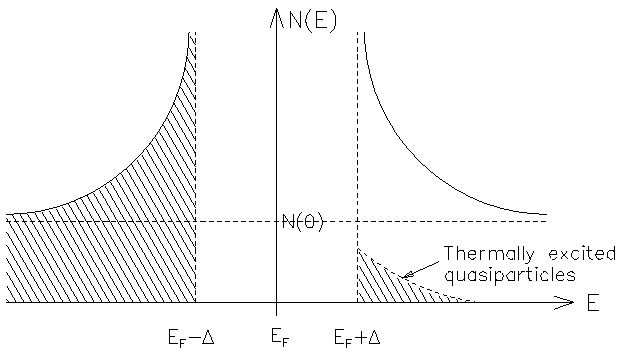
\includegraphics[width=.8\textwidth]{immagini/Densita_degli_stati_superconduttore.png}
\end{figure}
%This gap depends on temperature and it becomes zero at the critical temperature. Basically, what happens increasing the temperature going from zero temperature to the critical temperature is that at the critical temperature the superconductor becomes again a normal metal and then the density of states becomes the one we know for a normal metal. We can see the behavior of the gap as a function of temperature with this gap closing at the critical temperature in the following picture:
\hspace{-0.6cm}Questo gap dipende dalla temperatura e si annulla alla temperatura critica. In pratica, ciò che accade aumentando la temperatura da zero fino alla temperatura critica è che, alla temperatura critica, il superconduttore ritorna ad essere un metallo normale, e la densità degli stati torna ad essere quella che conosciamo per un metallo normale. In altre parole, man mano che aumentiamo la temperatura il gap si restringe, fino a chiudersi in corrispondenza della temperatura critica.\\
Possiamo osservare l'andamento del gap in funzione della temperatura, che si chiude alla temperatura critica, nella seguente figura:
\begin{figure}[H]
   \centering
   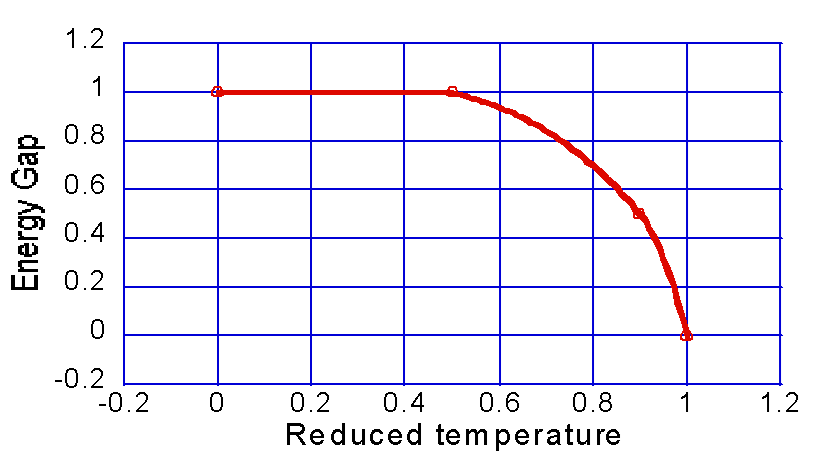
\includegraphics[width=.6\textwidth]{immagini/Andamento_gap_in_funzione_di_T.png}
   \caption*{Andamento del rapporto $\frac{\Delta(T)}{\Delta(0)}$ in funzione della temperatura ridotta $\frac{T}{T_c}$.}
\end{figure}
%The appearance of a gap in the spectrum has also other evidences. In particular, another evidence comes from the spectroscopic measurements of the absorption of electromagnetic radiation by a superconductor. In general, if we have a material and we make it interact with the electromagnetic field, what happens is that some frequencies are absorbed and the absorption spectrum depends intrinsically on the spectrum of the material hence on its density of states. If there are gaps in the spectrum, it means that the system cannot absorb energies smaller than the energy gap, and indeed measurements of absorption of electromagnetic radiation by a superconductor relieved that there was an onset of absorption for frequencies which are larger than an energy scale. Moreover this energy scale, which now we know is related to the superconducting gap, was scaled with the critical temperature, with a very simple expression: $\hbar\omega \approx k_B T_c$. So this experiment, which came out a little bit later with respect to the first observation, are part of the indication of the fact that in the spectrum of the superconductor there are some energies which cannot be taken simply because the system material is not able to absorb energy smaller than an energy scale, which is proportional to $k_B T_c$.\\
\hspace{-0.6cm}La comparsa di un gap nello spettro ha anche altre evidenze sperimentali. In particolare, un'altra evidenza proviene da misure spettroscopiche dell'assorbimento di radiazione elettromagnetica da parte di un superconduttore. In generale, se abbiamo un materiale e lo facciamo interagire con un campo elettromagnetico, ciò che accade è che alcune frequenze vengono assorbite, e lo spettro di assorbimento dipende intrinsecamente dallo spettro del materiale, e quindi dalla sua densità degli stati. Se ci sono dei gap nello spettro, significa che il sistema non può assorbire energie inferiori al valore del gap, e infatti le misure di assorbimento di radiazione elettromagnetica da parte di un superconduttore hanno rivelato che l'assorbimento inizia solo per frequenze superiori a una certa scala energetica. Inoltre, questa scala energetica (che ora sappiamo essere legata al gap superconduttivo) risultava proporzionale alla temperatura critica, secondo la relazione $\hbar \omega \approx k_B T_c$.\\
Questi esperimenti, che sono arrivati poco dopo le prime osservazioni del fenomeno, sono una chiara indicazione del fatto che nello spettro di un superconduttore esistono energie che non possono essere assorbite, semplicemente perché il materiale non è in grado di assorbire energia al di sotto di una determinata soglia, proporzionale a $k_B T_c$.\\
%Another evidence of this gap in the spectrum comes from the measurements of current--voltage relation, that is the relation between the current flowing in a superconducting material varying the applied voltage difference. These experiments were not done on a single superconductor but in a structure, which we will study in more depth in the following, which is composed by a normal metal, then some barrier so some insulating layer, and a superconducting material like the following picture:
Un'altra evidenza della presenza del gap nello spettro proviene dalle misure della relazione corrente--tensione, cioè dalla relazione tra la corrente che fluisce in un materiale superconduttore al variare della differenza di potenziale applicata.
Questi esperimenti non sono stati condotti su un singolo superconduttore, ma su una struttura (che analizzeremo più in dettaglio in seguito) composta da un metallo normale seguito da una barriera (ossia uno strato isolante) e infine da un materiale superconduttore. Vediamo la struttura dei livelli energetici di una tale configurazione:
\begin{figure}[H]
   \centering
   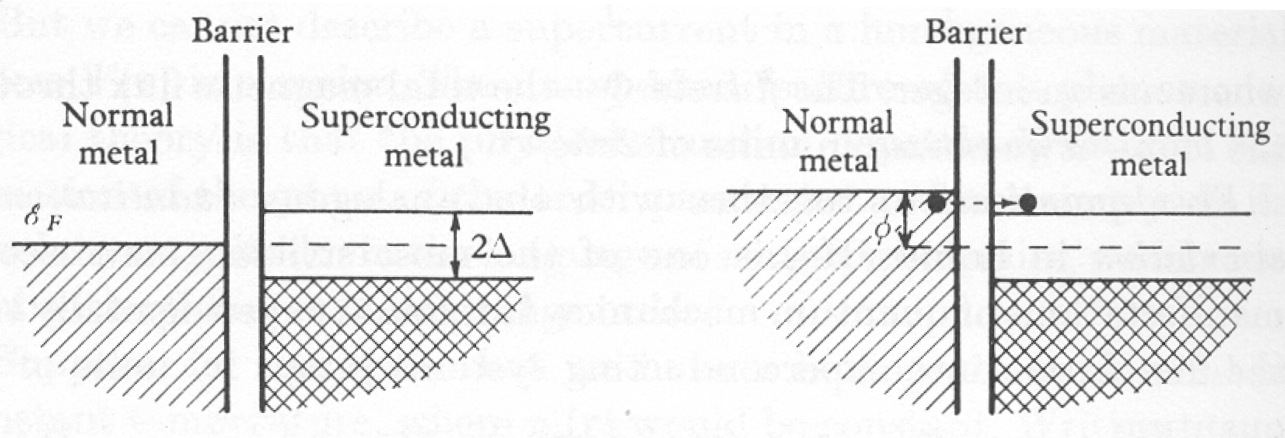
\includegraphics[width=.9\textwidth]{immagini/Electron_tunneling.png}
\end{figure}
%As we know, for a normal metal at zero temperature all the levels up to the Fermi energy are filled, and above there are all levels accessible by excitation. If instead in the superconductor\mn{Let's remark that at this stage we still don't know the reason, so we're assuming the superconductive spectrum has this gap.} we have all the levels filled up to some energy, and then there is an energy gap which separates the allowed states, and if the the levels of the two materials are like in the left configuration, if we do not apply a voltage between them an electron of the metal near the Fermi energy cannot pass\mn{This passing from one side to the other means passing an area where there is an insulating material that in terms of quantum mechanics represents a potential barrier, so this passage from one side to the other is by a quantum mechanical tunneling through a potential barrier.} to the other side because it doesn't have an available state on the other side.\\
%If we apply a potential difference, which can be described as a relative shift of the energy levels, in such a way that the Fermi level on the left-hand side is aligned, using the language of semiconductors, with the lower level of the upper band, so if we have a situation like the one in the right, under this condition an electron of the metal can tunnel through the barrier and find an available energy state on the other side. This means that if we want to see how the current--voltage characteristics looks like, this behavior means that if the voltage is smaller than an energy of the order of $\Delta$, there cannot be current because there are no available states on the other side, so there is zero current, and if the voltage is sufficient to unbalance the two bands in the proper way, at this point there will be a current flowing. So what we observe is a behavior like this:
\hspace{-0.6cm}Come sappiamo, per un metallo normale a temperatura nulla, tutti i livelli fino all'energia di Fermi sono occupati, e al di sopra ci sono tutti i livelli accessibili tramite eccitazione.
Nel superconduttore\sn{Ricordiamo che a questo punto non conosciamo ancora la causa di questo comportamento: stiamo semplicemente assumendo che lo spettro di un superconduttore presenti un gap.}, invece, tutti i livelli sono occupati fino a una certa energia, e poi c'è un intervallo di energia proibito che separa gli stati permessi. Se i livelli energetici dei due materiali sono disposti come nella configurazione a sinistra, in assenza di una differenza di potenziale tra loro, un elettrone nel metallo vicino al livello di Fermi non può passare dall'altra parte\sn{Questo passaggio da un lato all'altro significa attraversare una regione in cui è presente un materiale isolante, che in termini della meccanica quantistica rappresenta una barriera di potenziale e quindi il passaggio è un effetto di tunneling quantistico attraverso una barriera.}. Se applichiamo una differenza di potenziale, che può essere descritta come uno spostamento relativo dei livelli energetici, in modo che il livello di Fermi sul lato sinistro sia allineato, usando il linguaggio dei semiconduttori, con il livello inferiore della banda superiore, cioè in una configurazione come quella mostrata a destra, allora un elettrone del metallo può attraversare la barriera tramite tunneling e trovare uno stato disponibile sull'altro lato.\\
Ciò implica che finché la tensione applicata è inferiore a un'energia dell'ordine di $\Delta$ non può esserci passaggio di corrente, perché non ci sono stati accessibili sull'altro lato. Quando invece la tensione è sufficiente a sbilanciare in maniera opportuna i due spettri, inizia ad esserci passaggio di corrente. Pertanto, il comportamento corrente--tensione che si osserva sperimentalmente è come quello riportato nel seguente grafico:
\begin{figure}[H]
   \centering
   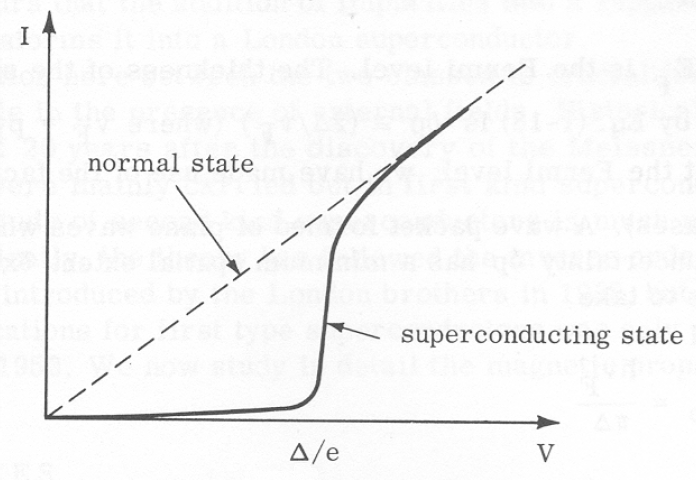
\includegraphics[width=.6\textwidth]{immagini/Grafico_tensione_corrente_Electron_tunneling.png}
\end{figure}
\hspace{-0.6cm}Come possiamo vedere, c'è una variazione brusca della corrente vicino a un'energia che è proporzionale al gap energetico. Se aumentiamo ulteriormente la tensione, il che significa che sbilanciamo ulteriormente i livelli energetici, possiamo, in un certo senso, dimenticare che un materiale è superconduttore ed è come se avessimo semplicemente due metalli normali, con il tunneling elettronico che può avvenire, quindi abbiamo una caratteristica corrente-tensione lineare, come in un sistema ohmico.\\
Questo comportamento, in cui si ha il passaggio di corrente soltanto se la differenza di potenziale supera un certo valore, è detto di attivazione. La presenza di questo comportamento ci porta a pensare che nello spettro di un materiale superconduttore ci sia un gap.
\subsection{Effetto isotopico}
%Another peculiarity of superconductors is called isotope effect. It was observed that the critical temperature to which the material becomes superconductive, depends on the mass of the isotope of the material. In other words, different isotopes of the same material have different critical temperature, following the law
%with $\alpha \approx 0.5$.\\
%The various isotopes differ from each other for the mass of the ions, which form the lattice of the material. So it's not the property of the electrons in the material, but of the lattice. This was quite astonishing because it indicated that superconducting phase transition, a property which is intrinsically related to electromagnetic properties, so conduction properties, which we are used to relate to electrons, depends on properties of the lattice. This fact was completely unexplained until Frölich in 1950, had the intuition that the mechanism behind superconductivity might be related to the interaction of electrons with the phonons, so with the lattice vibrations. This was the precise intuition which led Bardeen, Cooper and Schrieffer to develop their theory which is based on the idea that two electrons with opposite charge and momentum can actually interact with an attractive interaction which comes from the common interaction with the lattice. We will see more precisely later on, but we have to keep in mind that the isotope effect was the incipit which gave the idea that some mechanism of interaction between electrons and phonons could be the key to the superconductivity.
Un'altra peculiarità dei superconduttori è chiamata effetto isotopico. È stato osservato che la temperatura critica alla quale il materiale diventa superconduttore dipende dalla massa dell'isotopo del materiale. In altre parole, isotopi diversi dello stesso materiale presentano temperature critiche diverse, seguendo la legge:
\begin{equation*}
   T_c \propto M^{-\alpha}
\end{equation*}
con $\alpha \approx 0.5$.\\
I diversi isotopi si distinguono tra loro per la massa degli ioni che costituiscono il reticolo del materiale, quindi non si tratta di una proprietà degli elettroni nel materiale, ma del reticolo stesso. Questo fatto fu piuttosto sorprendente, perché indicava che la transizione alla fase superconduttiva, cioè una proprietà intrinsecamente legata all'elettromagnetismo, quindi alla conduzione elettrica, che siamo abituati ad associare agli elettroni, dipende invece da una proprietà del reticolo.\\
Questo fatto rimase del tutto inspiegato fino a quando, nel 1950, Fröhlich ebbe l'intuizione che il meccanismo alla base della superconduttività potesse essere legato all'interazione degli elettroni con i fononi, ovvero con le vibrazioni del reticolo. Questa fu l'intuizione decisiva che portò Bardeen, Cooper e Schrieffer a sviluppare la loro teoria, basata sull'idea che due elettroni con carica e momento opposti possano interagire tra loro attraverso un'interazione attrattiva mediata dall'interazione comune con il reticolo.\\
Vedremo più in dettaglio questo aspetto in seguito, ma dobbiamo tenere a mente che l'effetto isotopico fu l'elemento iniziale che fece intuire che un meccanismo di interazione tra elettroni e fononi potesse essere la chiave per spiegare la superconduttività.
%\subsubsection*{Altre informazioni sugli elementi superconduttori (da sistemare)}
%, so this is what we want to tell. we think there are some more information. , from the periodic table, you can now see how many materials in this placement of activity. And you can see the colors are all superconductive materials. So they are not just the standard aluminum, they could be, et cetera. But a large number of materials are superconductive, either under ambient pressure or under high pressure. And this is the reason for the colors. You see here the different temperatures. These are called small temperatures. So, let's say the materials from the periodic table are typically low-temperature materials. But if we analyze the this is, for instance, starting with a stable, the different materials which by now is placed by conductivity, we see that beside elements which are the ones we can find in the periodic table, there are also compounds which display superconductive behavior. And in particular, these compounds, which are typically ceramic materials, display superconductivity at much higher temperatures. You see that here we reach 100 Kelvin. So, much higher temperature with respect to the conventional or normal temperatures. These materials are called high-temperature superconductors. We won't enter the limits of the high-temperature superconductors, also because the theory behind high-temperature superconductors is not totally accepted. But this is just to show you this graph you see as a function of years, the different critical temperatures.
%\begin{figure}[H]
%   \centering
%   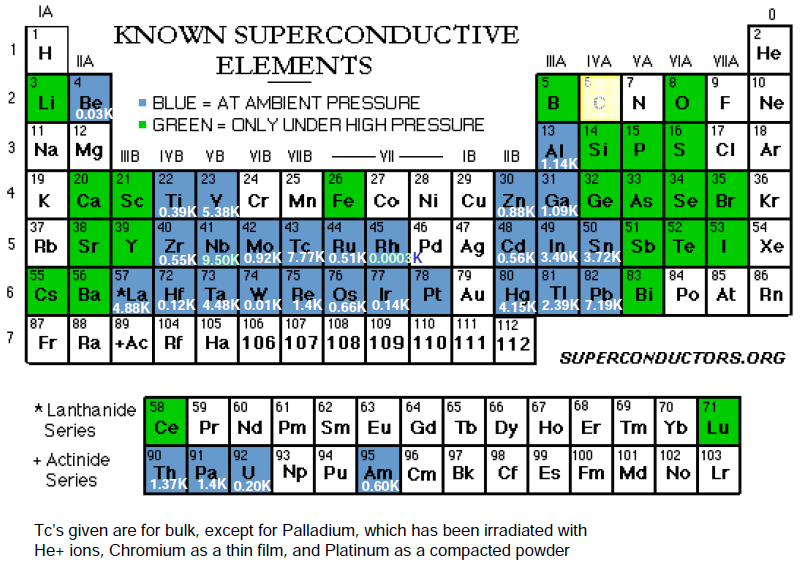
\includegraphics[width=.8\textwidth]{immagini/Tabella_elementi_superconduttivi.png}
%\end{figure}
%You see that there was a there were also were the 80s, late 80s, a discovery of these materials, which are based on they are basically some of the they are ceramic and are characterized by having layered structures of copper or oxide planes, which are separated by layers of, so to speak, chargers and warzones, which are your materials like, and the ones you see here. So, yeah, they have this layered structure and they display superconductivity but at much higher temperatures with respect to the bare elements. The theory behind high-temperature superconductors is not totally accepted, and particularly is not clear, which is the mechanism which needs the superconductivity, so we will not enter this part where you write to know the process of superconductivity in the view that also exists high-temperature superconductivity, and you keep in mind that the mechanism behind that is considerably different from the microscopic one, which we are now going to describe in the next lectures. And, , this is just a summary of what we have said today, and the interest, just to say that the interest for high-temperature superconductors, of course, comes from the applications, because we would really, of course, materials which are zero resistivity and in this phase, a temperature which are much higher than the cryogenic temperatures are, of course, interesting for all applications. So, there is clearly an interesting understanding in using these materials, but still there are some contrasts in using them. First of all, the fact that these players material are very sensitive to fluctuations, and so it means that they are not stable enough to allow an explosion in them, and you understand. , so we think that for the moment we , we will, maybe next time, we discuss about the qualitative features of the experiment. , so today we stop here, and the slides that are available, we have only done a new overview of phenomenology, and what is important to have in mind is, let's say, the only thing that we have done is to introduce the thermodynamic potentials that allow us to describe the transition, in particular the energy for the teams, and this has allowed us to introduce the thermodynamic definition of the field. This part here is good, because we will use it in the description of the theory of Ginzburg--Landau, which is based on the theory of Landau and the transition of phases. The second tip is that we that use the terminology and the terms of free energy, and the transition of things. So, this part here is important for the work of the idea of the experiment. And to address the thermodynamic potential, the difference between the fact that the Meissner effect cannot be explained with a perfectly conductive behavior and a simple explanation based on the analysis of the law of doing a perfect conductor, a simple point of point to understand the difference. . . No, no, no. So, a conductor is not a perfect conductor, because this is not is But to say resistivity with nothing resistivity. Yes. , perfect. The resistivity is zero of the first equation, which is that this resistivity has nothing to do with the Meissner effect, that is, the response to a magnetic field is not perfect. This is perfect. It is not a perfect conductor. It conductor. It conductor. perfect conductor that loses its internal voltage if this field is the last one. Yes, yes. We have this one, which means that a master should be able to see the distance.
%\section{Superfluidità (da sistemare)}
%Superfluidity is the property which some systems, actually $\rm ^3He$ and $\rm ^3He$ so far, which under proper conditions of temperature, magnetic field and pressure sustain the flow without friction, in the sense of without any viscosity. This takes place for certain temperatures as we said and up to certain transport velocities that are in this room. Now today, the only materials which display this Bm are $\rm ^4 He$ and $\rm ^3 He$. The first one is superfluid at about 2 K, the second one at much smaller temperature, and indeed it was discovered some years ago. And the experiments which demonstrated this superfluid behavior are again, also in this case, online, called thermodynamic and off-transport. Actually what was surprising and was to some extent is still not completely understood is the the that these two isotopes of helium are actually characterized by many different statistics, not only different atomic masses. And this of course makes the understanding of the phenomenon quite complicated. In particular, as we said, $\rm ^4 He$ has zero nuclear spin, therefore it's the bosonic natural base, those are statistics, whereas $\rm ^3 He$ has a nuclear spin which is an integer, so it obeys the media statistics. Now the first experiments, so helium-4, was done in 1930 by Fabitza, and the property was related to, it was a transport property, and it concerned the transport of helium through a narrow cabilla, and it was possible to see that this transport through this narrow cabilla was placed without any friction. And how did they understand that there was no friction, simply because for a viscous, it would be a fluid, a normal fluid, there is a connection between the difference in pressures on the two sides of the cabilla, and the coefficients eta, which describes this possibility. And actually what it was observed is that under this condition, there was no change in the pressure on the two sides of the cabilla, which was an indication of the fact that there was a super fluid. The other property, which is a game of sort of mechanical origin, is the observation of a stack of different disks, which were immersed in helium, and it was possible to see that the torsional, the torsional properties, so the oscillation frequency of this task, or stack of disks, was depending on the temperature of the system overall, and it appeared that for temperature below a certain value, the moment the inertia of the disk was changing, and this inertia was changing in such a way that apparently part of the disks were not involved. So this means, this is due to the fact that there is this fluid, which which in between the disks, becomes super fluid, and then the overall stack of disks is not anymore as single as the object, as it would be if there was a friction, but they were almost independently moving. So this was another indication. So these are, so to speak, mechanical mechanical The other peculiar feature of the loophole is the phase diagram, and in the phase diagram, which is shown out there, we have the pressure and the temperature, and the peculiarity is the following. So we have these different phases, which are a solid phase, for small temperature and sufficiently high pressure. We have a normal liquid behavior for pressure and temperature above certain pressure, but for small temperatures and for small values of the pressure, there is a super fluid behavior. And in particular, we see that differently from the usual transition we have in a fluid, where we have a tripod point between the three phases, there is no tripod point in this case. There is a liquid phase down to zero, which is surprising. And moreover, there is the peculiarity in the dependence on this phase, which separates this line, which separates the two phases, which is flat. And this is a relevant information because the dependence of the pressure on the temperature enters the entropy. So if we have a flat dependence on the pressure on the temperature, it means that there is no change in the entropy. Or if you want, this is a line where the entropy does not change, which indicates that we are passing from the liquid, the solid, there is no change in entropy. So it means that it gives us information about the structure, if you want, of the liquid, meaning that it has the same symmetry, the same entropy, the same order, the little profile of the solid phase.
%So this is quite the peculiarity. Moreover, if we, the space diagram translates in a peculiar dependence on the specific heat, of the specific heat of temperature, with a T-cube behavior, as more temperatures, which is different from what one observed for a bosonic condensation, you don't know, but just to notice that this is not the same as it happens in a bosonic condensation, which in principle, one may, at first instance, one could think that being a bosonic system, the same mechanism could happen, also in this case, but this is not the case. And the dependence of the specific heat on temperature is an indication that this is not the case. And moreover, there is this peculiar sort of spike here at the critical temperature, at the transition point. This point is called the lambda point, because of the shape of this curve. And this peculiar algebraic behavior close to the critical temperature, this type of behavior is an indication of the fact that between the normal liquid and the superfluid, there is a phase transition with two components of the parameter. Again, this is something which is not obvious, I'll just say with this problem, at this moment, just to let you know that there is some peculiar model behind this type of transition. , so these are just hints of the fact that in addition to the properties of a superconductor, which we have seen of Lady, are to the resistivity and the dependence and the expulsion of the documented field out of the sample, superfluids have quite different properties, quite different evidence in experiments both in transport, mechanical response, and in thermal properties. As you can see also in this case, the thermal properties are very important. Similarly, we have seen in the report a very important indicator of a transition, the characteristics of the transition. We will come later to the explanation with different features. At this stage, just to give you an idea of the variety of phenomena, which indicated some peculiar property, some peculiar phenomenon. 
\section{Equazione di London}
Iniziamo la trattazione dei superconduttori partendo dalle teorie fenomenologiche. Il motivo per cui utilizziamo queste ultime non è solo storico, ma anche perché si tratta di modelli semplici che permettono comunque di descrivere una grande varietà di fenomeni e che vengono ancora utilizzati per analizzare dispositivi superconduttivi semplici.\\
La prima teoria fenomenologica è l'equazione di London, formulata dai fratelli London nel 1935. Fu la prima teoria in grado di spiegare l'espulsione del campo magnetico dai superconduttori, ovvero l'effetto Meissner. L'idea alla base di questa teoria è molto semplice: i London furono motivati dall'osservazione che, al di sotto di una certa temperatura, la resistività del mercurio diventava nulla. L'ipotesi più immediata che si potesse fare era che il metallo fosse composto da elettroni suddivisi in due "fluidi", con una parte di elettroni che si comportava come normali elettroni, quindi con resistività finita, e un'altra parte che per qualche ragione diventava superconduttiva. L'idea è quindi che la densità totale di elettroni sia data dalla somma di un contributo normale $n_n$ e di un contributo superconduttivo $n_s$:
\begin{equation}
   n=n_n + n_s
   \label{eq:densita_elettroni}
\end{equation}
Tale modello a due fluidi si ispirava a un modello già proposto per l'$^4\rm He$, ma per ora possiamo accantonare questo aspetto.\\
L'assunzione fondamentale del modello di London è, dunque, che in un superconduttore coesistano elettroni normali ed elettroni superconduttivi. Se immaginiamo un sistema composto da due componenti fluide, e assumiamo che al di sotto della temperatura critica la componente superconduttiva sia presente, allora possiamo trattare il contributo degli elettroni normali e superconduttori come un sistema di trasporto con due canali in parallelo. Chiaramente, se uno dei due canali ha resistività nulla mentre l'altro ha resistività finita, il trasporto della corrente avverrà interamente attraverso il canale a resistività nulla. Viceversa, quando il sistema supera la temperatura critica o quando le condizioni del campo magnetico sono tali che il materiale si trova in fase normale, rimane un unico canale con resistività finita, e il materiale si comporta come un normale conduttore. Il motivo per cui la modellizzazione del problema è questa è che la teoria di London si propone di spiegare la fenomenologia superconduttiva, e questa fenomenologia include il fatto che se aumentiamo la temperatura nel materiale avviene il passaggio da superconduttore a metallo normale. Quindi, se abbiamo due fluidi con questi due comportamenti diversi al di sotto della temperatura critica, gli "elettroni superconduttivi" sono quelli responsabili della corrente.\mn{Ciò che avviene è che gli elettroni superconduttivi "cortocircuitano" gli elettroni normali e fanno crollare la resistività a zero. \cite{Annett}}
%We talk about superconductors starting from phenomenological theories. The reason why we use these phenomenological theories until now are not just for historical reasons, but also because they are simple theories which still allow us to describe a variety of phenomena which still we use when we consider very simple superconducting devices.\\
%The first phenomenological theory is the London equation, it's due to the London brothers on 1935. It was the first theory which could explain the expulsion of the magnetic field out of the superconductors, that is the Meissner effect. The idea behind this is very simple: they were motivated by the observation that below some certain temperature, the resistivity of Mercury went to 0, and the simplest instance which one could suppose is that the metal was formed by electrons described as two fluids, so considering part of the electrons behaving for some reason as normal electrons, so with normal resistivity and another part which for some unknown reason became superconductive. So, the idea is that we have a density of electrons given by a normal contribution plus a superconducting contribution. This two-fluid model was actually motivated from what was already proposed for $\rm ^4 He$, but let's keep it on one side of our mind. So the basic assumption of this London model is that in a superconductor, we have at the same time normal electrons with some density, which we call $n_n$, and superconducting electrons with some other density, which we call $n_s$. The total density is then given by
%\begin{equation*}
%   n=n_n + n_s
%\end{equation*}
%The idea is that if we have a system where we have these two fluid components, if for some reason (and this is the assumption) the superconducting component below the critical temperature is present, then we can think to the contribution of this normal and superconducting elements like a sort of parallel combination of two channels for transport. Clearly, if there is a channel which is with zero resistivity and the other with a finite resistivity, the transport takes place through the zero resistivity channel. Whereas, when the system is above the critical temperature or we have proper condition for the magnetic field such that it becomes normal, then we have a single channel with some resistivity and then we have the normal behavior, because this model is aimed to try to give an explanation of the superconducting phenomenology, and the phenomenology includes the fact that if we increase the temperature then the transition from superconducting to normal takes place in the material. So, if we have two fluids with these two different behaviors below the critical temperature, the "superconducting electrons" are the ones which are responsible for the current.
\subsection{Prima equazione di London}
%The equation which describes the supercurrent density is
%which tells us that current density is proportional to the vector potential with a coefficient which depends on the density of superconducting electrons, the charge of a single electron and the mass of a single electron.\\
%\eqrefcustom{eq:prima_equazione_di_London} is not enough: it applies in this model provided we are in a proper gauge, and in particular in the gauge which is called London gauge, which is characterized by having $\div{\vb{A}}=0$.\\
%Let's now try to understand how this equation comes from, which is the reason behind, and why it describes superconducting behavior and Meissner effect. Within this phenomenological model, this equation is the corresponding of Ohm's law for normal conductors, which states that for a normal conductor the current density is given by $\vb{J}=\sigma \vb{E}$. The idea is that if we have a superconductor this equation does not apply, because for $\rho \to 0$ we have $\sigma \to \infty$, which has not physical meaning. So Ohm's law has to be replaced by \eqrefcustom{eq:prima_equazione_di_London}.\\
%Now let's see how this equation comes from.\mn{Obviously, \eqrefcustom{eq:prima_equazione_di_London} is a phenomenological equation, so there is not a rigorous derivation, but of course the two London didn't invent it out of the blue: there is some reasoning behind it, so we will follow this reasoning and understand how we can describe the two characteristic phenomena, and then we will see some predictions from this.}\\
L'equazione che descrive la densità di corrente superconduttiva è la prima equazione di London, la quale afferma che
\begin{equation}
   \vb{J}=-\frac{n_s e^2}{m_e} \vb{A}
   \label{eq:prima_equazione_di_London}
\end{equation}
ossia che la densità di corrente è proporzionale al potenziale vettore $\vb{A}$ tramite un coefficiente che dipende dalla densità di elettroni superconduttivi $n_s$, dalla carica dell'elettrone $e$ e dalla sua massa $m_e$.\\
L'\eqrefcustom{eq:prima_equazione_di_London} da sola non basta: essa è valida all'interno di questo modello a patto di scegliere una gauge opportuna che è la gauge di London, caratterizzata dalla condizione $\div{\vb{A}} = 0$.\\
Vediamo da dove proviene la necessità di scegliere tale gauge. Sappiamo che, in generale, vale l'equazione di continuità:
\begin{equation*}
   \pdv{\rho}{t} + \div{\vb{J}} = 0
\end{equation*}
Se ci troviamo in condizioni di corrente continua (DC), allora $\pdv*{\rho}{t}=0$, e l'equazione di continuità diventa $\div{\vb{J}}=0$. Se inoltre $\vb{J}$ è proporzionale ad $\vb{A}$, come supposto dall'equazione di London, allora necessariamente deve valere anche $\div{\vb{A}}=0$, che è proprio la gauge di London. Quindi, la necessità di scegliere tale gauge nasce direttamente dall'assunzione di una densità di corrente proporzionale ad $\vb{A}$, insieme alla condizione di corrente continua.\\
All'interno di questo modello fenomenologico, questa equazione rappresenta l'equivalente della legge di Ohm per i conduttori normali, la quale stabilisce che in un conduttore normale la densità di corrente è data da $\vb{J}=\sigma \vb{E}$. L'idea è che se abbiamo un superconduttore, questa equazione non è più valida, perché nel limite di resistività nulla $\rho \to 0$, la conduttività $\sigma$ diverge, $\sigma \to \infty$, il che non ha significato fisico. Quindi la legge di Ohm deve essere sostituita dall'\eqrefcustom{eq:prima_equazione_di_London}.
\subsection{Derivazione dell'equazione di London}
Vediamo ora da dove proviene questa equazione, quale ne è il fondamento e perché descrive il comportamento superconduttivo e l'effetto Meissner. Prima di proseguire, va notato che tale equazione è stata ricavata anche dalla teoria BCS circa vent'anni dopo. Questo fatto ci dà un'indicazione di quanto essa sia rilevante: pur essendo stata ottenuta, come vedremo, sotto ipotesi non del tutto giustificate e principalmente motivata dal bisogno di avere una teoria fenomenologica capace di spiegare i risultati sperimentali, essa può comunque essere dedotta anche da una teoria microscopica. Questo fornisce quindi una giustificazione del perché questa equazione rimanga valida: non è solo un'intuizione empirica, ma trova fondamento anche in una descrizione teorica più profonda.\\
Cerchiamo innanzitutto di capire come si giunge a questa equazione.\sn{Ovviamente, l'\eqrefcustom{eq:prima_equazione_di_London} è un'equazione fenomenologica, quindi non esiste una derivazione rigorosa, ma chiaramente i fratelli London non l'hanno inventata dal nulla: c'è un ragionamento alla base, che ora seguiremo per capire come essa descriva i due fenomeni caratteristici della superconduttività, e vedremo anche alcune previsioni che ne derivano.}
Partiamo dalla considerazione che, tipicamente, ciò che diventa superconduttore è un metallo, e sappiamo che in un metallo, in condizioni normali, vale la legge di Ohm, cioè $\vb{J} = \sigma \vb{E}$. Questa equazione è valida fisicamente non solo in condizioni statiche, ma anche in presenza di variazioni temporali. Se, come di consueto per un metallo normale, vogliamo comprendere la risposta a un campo variabile nel tempo, ciò che facciamo è sviluppare in serie di Fourier sia il campo elettrico che la densità di corrente. Sappiamo quindi che, per valori finiti della frequenza, la risposta ha la forma:
\begin{equation}
   \vb{J} e^{-i\omega t}
   =\sigma(\omega) \vb{E} e^{-i\omega t}
   \label{eq:legge_di_Ohm_in_sviluppo_di_Fourier}
\end{equation}
La conducibilità dipende dalla frequenza. La sua forma esplicita deriva da una descrizione classica ed è data da:
\begin{equation*}
   \sigma(\omega)
   =\frac{n e^2 \tau}{m_e} \frac{1}{1 - i \omega \tau}
\end{equation*}
dove:
\begin{itemize}[leftmargin=0.5cm]
   \item $n$ è la densità di portatori di carica, che in un metallo normale sono gli elettroni normali;
   \item $e$ è la carica degli elettroni;
   \item $m_e$ è la massa degli elettroni\mn{Per convenzione, in questa definizione si usa la massa dell'elettrone libero nel vuoto, $m_e$, piuttosto che la massa efficace $m$.};
   \item $\tau$ è il tempo di vita medio degli elettroni mentre si muovono nel conduttore. Si tratta di un tempo di vita perché, nel modello di Drude, gli elettroni subiscono urti con gli ioni del reticolo e tra di loro, e $\tau$ rappresenta l'intervallo medio tra questi urti.
\end{itemize}
Come possiamo vedere, essa è una quantità complessa, dove la parte reale rappresenta la risposta resistiva del conduttore, mentre la parte immaginaria rappresenta la risposta induttiva. Quello che allora faremo adesso è separare la parte reale da quella immaginaria. L'idea è che, all'interno di questo modello, ci si aspetta che quando il materiale diventa superconduttore il tempo medio tra una collisione e l'altra diventi estremamente lungo, tendendo all'infinito. In questo limite, si ottiene che la risposta reale, cioè la parte reale della conducibilità che corrisponde alla risposta resistiva, tende a zero, e rimane soltanto la componente immaginaria. Questo è esattamente ciò che accade, e ora vedremo come funziona.\\
La parte reale della conducibilità è:
\begin{equation*}
   \Re [ \sigma(\omega) ]
   =\frac{n e^2 \tau}{m_e} \frac{1}{1 + \omega^2 \tau^2}
\end{equation*}
%It's clear that if $\tau \to \infty$ then $\Re [ \sigma(\omega) ] \to 0$ and this is what we expect for a normal conductor: if the average time between collisions goes to infinity, the material is not resistive anymore and we only have the imaginary response.\\
%Let's come back to the case when we have a finite $\tau$. In this case, we also have what is called the sum rule, that says
%that is integrating over frequency $\Re [ \sigma(\omega) ]$ as a function of $\omega$ we get a constant independent of the lifetime $\tau$. This comes from the fact that if we look at this real part of the conductivity as a function of $\omega$, this is simply a Lorentzian which is centered in $\omega=0$ and with a width equal to $1/\tau$ and a maximum height equal to $\tau$.
È chiaro che se $\tau \to \infty$, allora $\Re [ \sigma(\omega) ] \to 0$, e questo è esattamente ciò che ci aspettiamo per un conduttore normale: se il tempo medio tra le collisioni tende all'infinito, il materiale non è più resistivo e rimane soltanto la parte immaginaria.\\
Torniamo ora al caso in cui $\tau$ è finito. In questo caso, vale anche quella che viene chiamata "sum rule" (regola di somma), che afferma:
\begin{equation*}
   \int_{-\infty}^{+\infty} \dd{\omega} \Re [ \sigma(\omega) ]
   =\frac{\pi n e^2}{m_e}
\end{equation*}
cioè, integrando rispetto alla frequenza la parte reale della conducibilità $\Re [ \sigma(\omega) ]$ come funzione di $\omega$, si ottiene una costante indipendente dal tempo di vita $\tau$. Ciò deriva dal fatto che, se consideriamo $\Re [ \sigma(\omega) ]$ come funzione di $\omega$, essa è semplicemente una curva lorentziana centrata in $\omega=0$, con una larghezza pari a $1/\tau$ e un'altezza massima pari a $\tau$.\\
Il fatto che l'integrale sia indipendente dal valore di $\tau$ significa che, anche se abbiamo questo comportamento limite in cui $\tau \to \infty$, questa sum rule deve comunque essere rispettata. Questo implica che tale relazione dovrebbe rimanere valida qualunque sia il valore di $\tau$. Tuttavia, abbiamo visto che per $\tau \to \infty$ la parte reale di $\sigma(\omega)$ si annulla per ogni $\omega$, quindi ne consegue che, per avere un integrale finito, $\Re [ \sigma(\omega) ]$ deve essere una funzione nulla quasi ovunque, ma con integrale finito. Questo succede se, sostanzialmente, $\Re [ \sigma(\omega) ]$ diventa una delta di Dirac centrata a frequenza zero:
\begin{equation*}
   \Re [ \sigma(\omega) ]
   =\frac{\pi n e^2}{m_e} \delta(\omega)
\end{equation*}
Quindi significa che, nel limite $\tau \to \infty$, la parte reale della conducibilità di un metallo normale diventa una delta di Dirac, mentre la parte immaginaria, in questo limite, diventa:
\begin{equation*}
   \lim_{\tau \to \infty} \Im [ \sigma(\omega) ]
   =-\frac{n e^2}{i \omega m_e}
\end{equation*}
Quello che facciamo ora è considerare un superconduttore come un conduttore normale con tempo medio tra collisioni infinito. Da quanto detto, ci aspettiamo che la sua conducibilità sia:
\begin{equation}
   \sigma(\omega)
   =\frac{\pi n_s e^2}{m_e} \delta(\omega) - \frac{n_s e^2}{i \omega m_e}
   \label{eq:conduttivita_superconduttore}
\end{equation}
Questo implicherebbe che, se fossimo in grado di misurare la parte reale della conducibilità in funzione della frequenza, dovremmo osservare solo un picco centrato a frequenza zero. In realtà, gli esperimenti mostrano che, effettivamente, la parte reale della conducibilità per un superconduttore ha un picco a frequenza zero, ma non si annulla per frequenze finite, come invece predirebbe l'\eqrefcustom{eq:conduttivita_superconduttore}. Infatti, si osserva un comportamento resistivo finito che compare al di sopra di una certa frequenza, come si vede nel seguente grafico:
\begin{figure}[H]
   \centering
   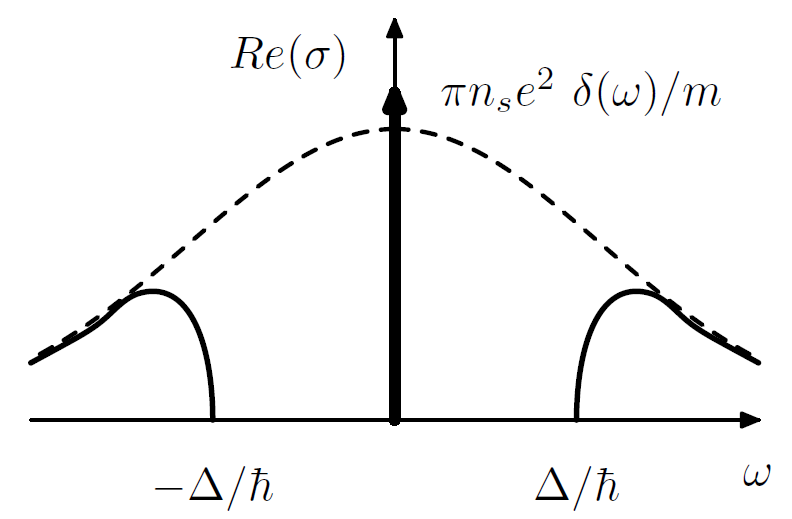
\includegraphics[width=.6\textwidth]{immagini/andamento_conducibilita.png}
   \caption*{Conducibilità a frequenza finita di un metallo normale (linea tratteggiata) e di un superconduttore (linea continua). Nel caso del superconduttore, un gap energetico porta a una conducibilità nulla per frequenze inferiori a $\Delta/\hbar$. Il peso spettrale rimanente si concentra in una funzione delta di Dirac in $\omega = 0$.}
\end{figure}
\hspace{-0.6cm}Tale comportamento conduttivo finito (che è simmetrico) somiglia molto a ciò che otterremmo dalla parte reale della conducibilità di un metallo normale. Infatti, possiamo vedere che coincide con la linea tratteggiata, che rappresenta il comportamento lorentziano tipico di un metallo normale. Oggi sappiamo che la frequenza in cui avviene questo cambiamento di comportamento corrisponde al gap superconduttivo, di cui abbiamo già parlato per un superconduttore.\\
Ciò significa che, se osserviamo la parte reale della conducibilità di un superconduttore, vediamo un picco a frequenza zero, seguito da una resistenza finita che compare a frequenze superiori a un certo valore caratteristico. Questo implica che, per frequenze superiori a tale valore, il sistema ha essenzialmente la stessa risposta di un metallo normale, per una ragione che, a questo punto, non possiamo ancora comprendere.\\
Supponiamo ora, seguendo questo ragionamento, di avere un materiale a resistenza zero, descritto da una conducibilità dipendente dalla frequenza come l'\eqrefcustom{eq:conduttivita_superconduttore} e andiamo a vedere quale forma ci si può aspettare per la densità di corrente. Quello che faremo sarà innanzitutto correlare questa densità di corrente $\vb{J}$ al potenziale vettore $\vb{A}$ (nel caso in cui venga applicato un campo magnetico, si noti che finora non è apparso alcun campo magnetico) e vedremo subito dopo che questa connessione tra $\vb{J}$ e $\vb{A}$ implica l'effetto Meissner.\\
Consideriamo l'\eqrefcustom{eq:legge_di_Ohm_in_sviluppo_di_Fourier} e calcoliamo il rotore di entrambi i membri:
\begin{equation*}
   \curl{\vb{J}} e^{-i\omega t}
   =\sigma(\omega) \curl{ \qty( \vb{E} e^{-i\omega t } ) }
\end{equation*}
Dalla legge di Faraday sappiamo che
\begin{equation*}
   \curl{\vb{E}}
   =-\pdv{\vb{B}}{t}
\end{equation*}
Possiamo sostituire nella precedente equazione, ottenendo
\begin{equation*}
   \curl{\vb{J}} e^{-i\omega t}
   =-\sigma(\omega) \pdv{t} \qty( \vb{B} e^{-i\omega t} )
   =i\omega \sigma(\omega) \vb{B} e^{-i\omega t}
\end{equation*}
Poiché stiamo considerando frequenze finite, la conducibilità ha solo la parte immaginaria\mn{Ricordiamo che ciò è dovuto alla presenza della $\delta(\omega)$, la quale implica che la parte reale è diversa da zero solo per frequenza nulla.}. Quindi l'equazione diventa
\begin{equation*}
   \curl{\vb{J}} e^{-i\omega t}
   =i\omega \qty( - \frac{n_s e^2}{i \omega m_e} ) \vb{B} e^{-i\omega t}
   =-\frac{n_s e^2}{m_e} \vb{B} e^{-i\omega t}
\end{equation*}
Prendiamo ora il limite per $\omega \to 0$, che significa considerare la risposta statica. Si ottiene
\begin{equation}
   \curl{\vb{J}}
   =-\frac{n_s e^2}{m_e} \vb{B}
   \label{eq:relazione_J_B}
\end{equation}
Sappiamo inoltre che il campo magnetico è in generale legato al potenziale vettore $\vb{A}$ tramite la relazione
\begin{equation}
   \vb{B}=\curl{\vb{A}}
   \label{eq:relazione_B_A}
\end{equation}
quindi possiamo riscrivere l'\eqrefcustom{eq:relazione_J_B} come
\begin{equation*}
   \curl{\vb{J}}
   =-\frac{n_s e^2}{m_e} \curl{\vb{A}}
\end{equation*}
Tuttavia, l'\eqrefcustom{eq:relazione_B_A} non identifica completamente il potenziale vettore in quanto essa è soddisfatta anche se aggiungiamo il gradiente di una funzione scalare $\chi$ ad $\vb{A}$. Per questa ragione, non possiamo immediatamente mettere in relazione $\vb{J}$ con $\vb{A}$, a meno di scegliere la gauge corretta per il potenziale vettore, che come abbiamo detto è la gauge di London. In conclusione, abbiamo che
\begin{equation*}
   \vb{J}
   =-\frac{n_s e^2}{m_e} \vb{A}
   \qq{se}
   \div{\vb{A}}=0
\end{equation*}
che è precisamente l'equazione di London che abbiamo dato in precedenza. Notiamo che la gauge di London è equivalente a considerare la condizione statica $\dv{\rho}{t}=0$.\\
In questo modo, abbiamo visto come, partendo dall'assunzione di avere un conduttore con resistività nulla, cioè un conduttore in cui una parte degli elettroni diventa superconduttiva, il che implica che la parte reale della conducibilità abbia la forma dell'\eqrefcustom{eq:conduttivita_superconduttore}, otteniamo una connessione tra la densità di corrente e il potenziale vettore.
\subsection{Spiegazione dell'effetto Meissner}
Vediamo ora come l'equazione di London sia in grado di prevedere l'effetto Meissner. Partiamo dalla legge di Ampere:
\begin{equation*}
   \curl{\vb{B}}
   =\mu_0 \vb{J}
\end{equation*}
Prendiamo il rotore di entrambi i membri:
\begin{equation*}
   \curl{(\curl{\vb{B}})}
   =\mu_0 \curl{\vb{J}}
\end{equation*}
Usando l'\eqrefcustom{eq:prima_equazione_di_London} e poi l'\eqrefcustom{eq:relazione_B_A}, possiamo scrivere:
\begin{equation*}
   \curl{(\curl{\vb{B}})}
   =-\mu_0 \frac{n_s e^2}{m_e} \curl{\vb{A}}
   =-\mu_0 \frac{n_s e^2}{m_e} \vb{B}
\end{equation*}
Notiamo che vale la relazione:
\begin{equation*}
   \curl{(\curl{\vb{B}})}
   =\grad{(\div{\vb{B}})} - \grad^2 \vb{B}
   =-\grad^2 \vb{B}
\end{equation*}
in quanto il campo magnetico è irrotazionale. Otteniamo quindi:
\begin{equation*}
   \grad^2 \vb{B}
   =\mu_0 \frac{n_s e^2}{m_e} \vb{B}
\end{equation*}
Se definiamo
\begin{equation}
   \lambda^2
   =\frac{m_e}{\mu_0 n_s e^2}
   \label{eq:lunghezza_di_penetrazione_London}
\end{equation}
che ha la dimensioni di una lunghezza al quadrato,\mn{Ci si può rendere conto che debba essere così per il fatto che a primo membro abbiamo l'operatore laplaciano, dunque affinché l'equazione sia consistente a livello dimensionale a destra dobbiamo avere l'inverso di una lunghezza al quadrato.} possiamo riscrivere
\begin{equation}
   \grad^2 \vb{B}
   =\frac{1}{\lambda^2} \vb{B}
   \label{eq:equazione_di_London_per_effetto_Meissner}
\end{equation}
L'\eqrefcustom{eq:equazione_di_London_per_effetto_Meissner} descrive precisamente l'effetto Meissner. Vediamolo esplicitamente in un caso semplice: supponiamo che lo spazio sia riempito da un superconduttore per $x>0$ e ci sia vuoto per $x<0$:
\begin{figure}[H]
   \centering
   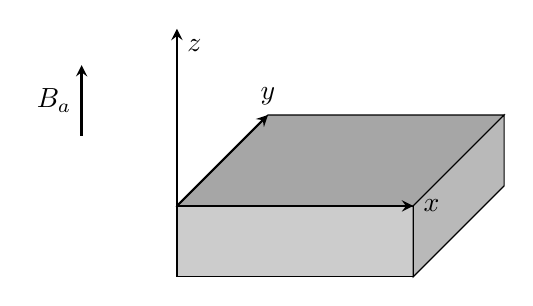
\begin{tikzpicture}[scale=1.5]
      %superconductor
      \draw[fill=gray!40] (0,0,0) -- (0,-.6,0) -- (2,-.6,0) -- (2,0,0) -- cycle;
      \draw[fill=gray!70] (0,0,0) -- (0,0,-2) -- (2,0,-2) -- (2,0,0) -- cycle;
      \draw[fill=gray!55] (2,0,0) -- (2,0,-2) -- (2,-.6,-2) -- (2,-.6,0) -- cycle;
      % Axes
      \draw[thick,-stealth] (0,0,0) -- (2,0,0) node[right] {$x$};
      \draw[thick,-stealth] (0,0,0) -- (0,1.5,0) node[anchor=north west] {$z$};
      \draw[thick,-stealth] (0,0,0) -- (0,0,-2) node[anchor=south] {$y$};
      % Campo magnetico
      \draw[thick,-stealth] (-1,.4,-.5) -- (-1,1,-.5) node[midway,left] {$\vb{B}_a$};
   \end{tikzpicture}
\end{figure}
\hspace{-0.6cm}Supponiamo di applicare nel vuoto un campo magnetico esterno $\vb{B}_a$ lungo la direzione $z$, ovvero $\vb{B}_a=B_z \vu{z}$, quindi parallelo alla superficie di contatto del superconduttore. Vediamo quale forma assume l'\eqrefcustom{eq:equazione_di_London_per_effetto_Meissner} in questa configurazione. Osserviamo innanzitutto che, poiché la componente parallela del campo magnetico non cambia attraversando l'interfaccia tra due mezzi, dovrà esserci un campo magnetico anche all'interno del superconduttore, diretto ancora lungo $z$.\\
Per prima cosa calcoliamo il termine $\grad^2 \vb{B}$:\mn{Per definizione, $\grad^2$ è dato dalla somma delle derivate seconde rispetto a $x$, $y$ e $z$ ma, considerando la simmetria del problema, non ci aspettiamo variazioni lungo le direzioni $y$ e $z$, mentre può esserci una variazione lungo $x$. Pertanto, l'operatore si riduce alla derivata seconda rispetto a $x$.}
\begin{equation*}
   \grad^2 \vb{B}
   = \grad^2 (B_z \vu{z})
   = \pdv[2]{B_z}{x} \vu{z}
\end{equation*}
Quindi, l'equazione di London per l'effetto Meissner diventa:
\begin{equation*}
   \pdv[2]{B_z}{x} \vu{z}
   =\frac{1}{\lambda^2} B_z \vu{z}
\end{equation*}
Ciò significa che la componente $z$ del campo magnetico deve soddisfare l'equazione
\begin{equation*}
   \pdv[2]{B_z}{x}
   =\frac{1}{\lambda^2} B_z
\end{equation*}
la cui soluzione è
\begin{equation}
   B_z(x)
   =B_z(0) e^{-x/\lambda}
   \label{eq:campo_magnetico_dentro_il_superconduttore}
\end{equation}
L'\eqrefcustom{eq:campo_magnetico_dentro_il_superconduttore} ci dice che, se osserviamo il profilo della componente $z$ del campo magnetico per $x>0$ ossia all'interno del superconduttore, vediamo che il campo magnetico parte da un valore finito in $x=0$, cioè esattamente sulla superficie, e poi decresce esponenzialmente all'interno del superconduttore su una lunghezza caratteristica pari proprio a $\lambda$.\\
\begin{marginfigure}
   \centering
   \begin{tikzpicture}
      \draw[->] (0,0) -- (4,0) node[right] {$x$};
      \draw[->] (0,0) -- (0,2.5) node[above] {$B_z(x)$};
      \draw[dashed] (1,0) node[below] {$\lambda$} -- (1,0.7357);
      \draw[thick,green!60!blue!] plot[domain=0:3.8,samples=100] (\x, {2*exp(-\x)});
   \end{tikzpicture}
   \caption*{Comportamento del campo magnetico all'interno di un superconduttore, in prossimità del bordo.}
\end{marginfigure}
\hspace{-0.35cm}Questo significa che, se abbiamo un superconduttore con questa particolare geometria immerso in un campo magnetico esterno (il campo applicato), all'interno del superconduttore non è presente campo magnetico. In altre parole, il campo che sarebbe presente se il materiale fosse normale viene espulso\sn{Notiamo che stiamo considerando la situazione finale: se potessimo osservare come si raggiunge questa condizione, vedremmo che raffreddando il superconduttore da temperature superiori alla temperatura critica a temperature inferiori ad essa, si passa da una situazione in cui il campo magnetico è uniforme in tutto lo spazio (compreso l'interno del metallo normale) a una in cui il campo viene praticamente espulso dal superconduttore, nel senso che solo una sottilissima regione sotto la superficie presenta ancora un campo magnetico finito, mentre il resto del materiale è caratterizzato da campo magnetico nullo.} e osserviamo che esso penetra soltanto in uno strato molto sottile sotto la superficie e, oltre una distanza dell'ordine di $\lambda$, il campo diventa praticamente nullo. Tale comportamento è esattamente quello che ci si aspetta dall'effetto Meissner.\\
Vediamo qual è il valore di $B_z(0)$. Come abbiamo detto, la componente parallela del campo magnetico non cambia attraversando una superficie, quindi il valore di $B_z$ in $x=0$ deve necessariamente essere uguale al campo applicato, quindi $B_z(0)=B_a$.\\
Possiamo osservare anche un altro aspetto. Descrivendo la fenomenologia di un superconduttore abbiamo detto che, se viene applicato un campo magnetico esterno, affinché il campo magnetico venga espulso deve esserci un'altra sorgente di campo magnetico che lo compensi esattamente. Abbiamo anticipato che ciò avviene perché sulla superficie del superconduttore si genera una supercorrente della quantità esattamente necessaria a generare un campo magnetico che compensi il campo applicato dall'esterno. Nella geometria dell'esempio che stiamo considerando, questo significa che, vicino alla superficie del materiale, esisterà un flusso di supercorrente tale da generare un campo magnetico opposto a $\vb{B}_a$. Ciò che faremo ora è calcolare la densità di corrente che scorre sulla superficie del superconduttore. Fare ciò è piuttosto semplice, perché abbiamo visto che esiste una relazione tra $\vb{J}$ e $\vb{A}$, o meglio tra $\curl{\vb{J}}$ e $\vb{B}$, data dall'\eqrefcustom{eq:relazione_J_B}. Poiché nel nostro caso il campo magnetico ha componente soltanto lungo $z$, possiamo considerare soltanto la componente $z$ del rotore di $\vb{J}$ e scrivere:
\begin{equation*}
   (\curl{\vb{J}})_z \vu{z}
   =-\frac{n_s e^2}{m_e} B_z \vb{z}
\end{equation*}
ovvero, esplicitando la componente del rotore,
\begin{equation*}
   \qty( \pdv{J_y}{x} - \pdv{J_x}{y} )
   =-\frac{n_s e^2}{m_e} B_z
\end{equation*}
Considerando la simmetria del problema, non ci aspettiamo una dipendenza da $y$ in quanto il sistema è simmetrico rispetto a tale direzione, quindi $\pdv{J_x}{y}=0$ e possiamo scrivere
\begin{equation*}
   \pdv{J_y}{x}
   =-\frac{n_s e^2}{m_e} B_a e^{-x/\lambda}
   =-\frac{\mu_0}{\lambda^2} B_a e^{-x/\lambda}
\end{equation*}
dove abbiamo esplicitato la forma del campo magnetico e poi utilizzato la definizione di $\lambda$ data dall'\eqrefcustom{eq:lunghezza_di_penetrazione_London}.\mn{Per ottenerla abbiamo moltiplicato e diviso per $\mu_0$.}\\
La soluzione di questa equazione è
\begin{equation*}
   J_y(x)
   =\frac{\mu_0}{\lambda} B_a e^{-x/\lambda}
\end{equation*}
In questo modo abbiamo dimostrato che esiste una densità di corrente, e quindi una supercorrente, che scorre lungo la direzione $y$, non nulla solo entro una regione di spessore $\lambda$ lungo la direzione $x$, cioè in uno strato del superconduttore parallelo al piano $xy$. Questa supercorrente genera un campo magnetico, diretto lungo $z$, che si può dimostrare essere tale da compensare esattamente il campo magnetico esterno applicato.
\subsection{Seconda coppia di equazioni di London}
A volte in letteratura, invece di trovare come definizione dell'equazione di London quella che abbiamo scritto nell'\eqrefcustom{eq:prima_equazione_di_London} associata alla gauge di London, si trova un'altra coppia di equazioni, che riguarda il rotore di $\vb{J}$ e la derivata temporale di $\vb{J}$. L'insieme di queste due relazioni è equivalente, come stiamo per dimostrare, all'\eqrefcustom{eq:prima_equazione_di_London} e alla gauge di London.\\
Consideriamo l'\eqrefcustom{eq:prima_equazione_di_London} e calcoliamo il rotore di entrambi i membri:
\begin{equation*}
   \curl{\vb{J}}
   =-\frac{n_s e^2}{m_e} \curl{\vb{A}}
\end{equation*}
Usando l'\eqrefcustom{eq:relazione_B_A}, possiamo scrivere
\begin{equation}
   \curl{\vb{J}}
   =-\frac{n_s e^2}{m_e} \vb{B}
   \label{eq:seconda_equazione_di_London}
\end{equation}
e l'\eqrefcustom{eq:seconda_equazione_di_London} è talvolta chiamata seconda equazione di London.\\
Prendiamo poi la derivata temporale dell'\eqrefcustom{eq:prima_equazione_di_London}:
\begin{equation*}
   \pdv{\vb{J}}{t}
   =-\frac{n_s e^2}{m_e} \pdv{\vb{A}}{t}
   %=-\frac{n_s e^2}{m_e} \vb{E}
\end{equation*}
Dall'elettromagnetismo sappiamo che, in generale, il campo elettrico può essere espresso come
\begin{equation*}
   \vb{E}=-\grad{\phi} - \pdv{\vb{A}}{t}
\end{equation*}
dove $\phi$ è il potenziale elettrico. Se $\phi$ è costante, possiamo scrivere
\begin{equation*}
   \pdv{\vb{J}}{t}
   =\frac{n_s e^2}{m_e} \vb{E}
   %=\frac{1}{\Lambda} \vb{E}
\end{equation*}
Se poniamo
\begin{equation*}
   \Lambda
   =\frac{m_e}{n_s e^2}
   %\label{eq:lunghezza_di_London}
\end{equation*}
possiamo scrivere
\begin{equation}
   \pdv{\vb{J}}{t}
   =\frac{1}{\Lambda} \vb{E}
   \label{eq:prima_equazione_di_London_alternativa}
\end{equation}
Talvolta, con prima equazione di London si intende l'\eqrefcustom{eq:prima_equazione_di_London_alternativa}.\\
Come possiamo vedere, l'\eqrefcustom{eq:seconda_equazione_di_London} e l'\eqrefcustom{eq:prima_equazione_di_London_alternativa} mettono in relazione la densità di corrente con il campo magnetico ed il campo elettrico, rispettivamente. C'è un punto importante da osservare: queste due equazioni non possono essere derivate l'una dall'altra. Infatti, non sono equivalenti, poiché forniscono due informazioni diverse sul superconduttore: una riguarda le proprietà di conduzione e l'altra riguarda le proprietà magnetiche, e come abbiamo già visto la conducibilità perfetta non implica l'effetto Meissner.\\
Ciò si può vedere partendo dall'\eqrefcustom{eq:prima_equazione_di_London_alternativa} e cercando di capire la risposta magnetica: se proviamo a farlo, vedremo che ciò non implica necessariamente l'effetto Meissner, che è una proprietà diversa. Per vedere tale fatto applichiamo il rotore all'\eqrefcustom{eq:prima_equazione_di_London_alternativa}:
\begin{equation*}
   \curl{\pdv{\vb{J}}{t}}
   =\frac{1}{\Lambda} \curl{\vb{E}}
   =-\frac{1}{\Lambda} \pdv{\vb{B}}{t}
\end{equation*}
dove nell'ultimo passaggio abbiamo usato la legge di Faraday. Portando tutto al primo membro otteniamo
\begin{equation*}
   \curl{\pdv{\vb{J}}{t}} + \frac{1}{\Lambda} \pdv{\vb{B}}{t}=0
\end{equation*}
Supponendo di poter scambiare l'ordine di derivazione rispetto al tempo e allo spazio, possiamo scrivere
\begin{equation*}
   \pdv{t} \qty( \curl{\vb{J}} ) + \frac{1}{\Lambda} \pdv{\vb{B}}{t}=0
\end{equation*}
e raccogliendo i due termini otteniamo
\begin{equation*}
   \pdv{t} \qty( \curl{\vb{J}} + \frac{1}{\Lambda} \vb{B} )=0
\end{equation*}
Confrontiamo tale relazione con l'\eqrefcustom{eq:seconda_equazione_di_London}: la prima ci dice che la quantità tra parentesi è costante ma non necessariamente nulla, mentre la seconda ci dice che è proprio nulla. Questo significa che la prima equazione di London, che descrive direttamente la risposta di una supercorrente a un campo elettrico, non è in grado di descrivere la risposta di un superconduttore a un campo magnetico, e in particolare l'effetto Meissner. Ne segue che, per mettere in relazione $\vb{J}$ sia con il campo elettrico che con il campo magnetico, sono necessarie sia la prima che la seconda equazione di London oppure, in alternativa, l'equazione di London che collega $\vb{J}$ al potenziale vettore $\vb{A}$ insieme alla gauge di London.\\
Derivation of \eqrefcustom{eq:prima_equazione_di_London_alternativa} for a perfect conductor is very intuitive if we use again a drude type description of the of the conductor. We know that Ohm's law can be derived if we consider the average response of the electrons in the presence of an external applied electric field:
\begin{equation}
   m_e \dv{\vb{v}}{t}
   =-e \vb{E} - \frac{m_e}{\tau} \vb{v}
   \label{eq:modello_di_Drude}
\end{equation}
This equation comes by considering the average motion of an electron to an applied electric field, including a viscous force describing the effect of the collisions which electrons suffer while moving in the conductor. If we consider in this regime the superconductor as a perfect conductor, meaning, as we said, that $\tau \to \infty$, it means that we have to neglect the damping term due to collisions, so \eqrefcustom{eq:modello_di_Drude} can be written as
\begin{equation*}
   -e n_s \dv{\vb{v}}{t}
   =\frac{e^2 n_s}{m_e} \vb{E}
\end{equation*}
where we have multiplied both members by $-\frac{e n_s}{m_e}$. We notice that the left hand side is just the derivative with respect to time of the current density $\vb{J}$, while in the right hand side we can recognize that the coefficient is equal to $1/\Lambda$, so this is precisely \eqrefcustom{eq:prima_equazione_di_London_alternativa}, that is the first London equation. So this is an equivalent way of deriving the two sets of the phenomenological London equations.\\
\subsection{La lunghezza di penetrazione di London}
\textbf{Nota: questa parte è da sistemare.}\\
Concentriamoci ora sulla previsione che possiamo ottenere dalla lunghezza di penetrazione di London. L'ordine di grandezza di $\lambda$ dipende dal materiale considerato. Come abbiamo visto, $\lambda$ è definita dall'\eqrefcustom{eq:lunghezza_di_penetrazione_London} e dipende da alcune quantità note con precisione e dalla densità degli elettroni superconduttivi $n_s$, che invece non conosciamo. Possiamo tuttavia stimare quest'ultima: poiché abbiamo assunto che la densità totale di elettroni in un superconduttore sia data dall'\eqrefcustom{eq:densita_elettroni}, possiamo ipotizzare che, nello stato superconduttivo, la frazione di elettroni normali sia trascurabile rispetto a quella degli elettroni superconduttivi.\\
Se questa ipotesi è valida, possiamo stimare che $n_s$ sia approssimativamente uguale alla densità totale di elettroni $n$. Quest'ultima deve coincidere con la densità elettronica del materiale nello stato normale, poiché, secondo il modello considerato, nel passaggio alla fase normale la densità di elettroni superconduttivi si annulla, lasciando invariata la densità totale di elettroni, che è quindi quella tipica del metallo normale, dell'ordine di $10^{22} \; \rm cm^{-3}$. Sulla base di questa stima, possiamo calcolare la lunghezza di penetrazione, che risulta, in queste condizioni, dell'ordine di 100 \A.\\
In realtà, gli esperimenti mostrano che $\lambda$ dipende dalla temperatura. Ciò significa che, ricavando da $\lambda(T)$ la corrispondente densità sperimentale $n_s(T)$, otteniamo una certa relazione funzionale. In particolare, si osserva che la dipendenza di $\lambda$ dalla temperatura segue una legge di potenza, che può essere espressa come:
\begin{equation*}
   \lambda(T)
   =\frac{\lambda(0)}{\sqrt{ 1 - \qty(\frac{T}{T_c})^{4}}}
\end{equation*}
Assumendo che a temperatura nulla tutti gli elettroni diventino superconduttivi, $\lambda(0)$ risulta proporzionale alla densità elettronica. Tuttavia, i dati sperimentali mostrano in genere che $\lambda(0)$ ha un valore dell'ordine di 500 \A, quindi maggiore rispetto alla stima teorica precedente.\\
%Let's now focus on the prediction we have from the London penetration depth. The order of magnitude of $\lambda$ depends on the material. As we have seen, $\lambda$ is defined by \eqrefcustom{eq:lunghezza_di_penetrazione_London} and it depends on some quantities we precisely know and on the density of superconductive electrons $n_s$, which we don't know. However, we can make an estimate: since our initial assumption is that the overall density of electrons in the superconductor is given by \eqrefcustom{eq:densita_elettroni}, we can assume that when the material is superconductive, the fraction of normal electrons is negligible with respect to the fraction of superconductive electrons. If this is the case, and this is an assumption, we can estimate that $n_s$ is almost equal to the density of electrons $n$, which must be the same as the density of electrons we have when the system becomes a normal metal because in the other regime, according to this model, the superconductive electrons density vanishes for some mysterious reason and the overall density of electrons is the one of the normal metal, which is a quantity we know and which is of the order to $\rm 10^{22}/cm^3$. So, according to this estimate, we can evaluate the penetration depth, which turns out to be, with this assumption, of the order of 100 \A.\\
%Actually, what we see from experiments is that $\lambda$ depends on temperature, so this means that if we extrapolate from the experimental $\lambda(T)$ an experimental $n_s(T)$ we will get some form. In particular, we find that $\lambda$ depends on temperature with the power law, which can be extrapolated to be

%So, assuming that at zero temperature all electrons becomes superconducting, then in this case $\lambda(0)$ is proportional to the density of electrons. Actually, experiments tipically give for $\lambda(0)$, a quantity which in general is the order of $500 \A$, so they give a larger value.
%%
This larger penetration depth can be predicted by refining the model, and the way this model is refined is similarly to what is done for a normal conductor, where instead of describing its response in terms of the Drude model, leading to the Ohm's law, we describe the non-local response of a normal metal which will bring a non-local response also for a superconductor.\\
\textbf{c'è una parte commentata da sistemare qui sotto}\\
%Qualitatively what we will do is the following: so far, we considered, with the Drude model, a local response, which means that if we are in a metal and we have an electric field in one point, precisely at the same point we will have a current density $\vb{J}$, which is given by $\vb{J}=\sigma\vb{E}$. Non local response means that the current density we will have in some point is not depending only on the electric field at the same point, but it depends on the electric field in some area, with some length scale, which depends on this area, which is depending on how we describe it. The result is that we have a question. Do you expect this J-prime to be larger or smaller than J? Depending on the field Well, if it depends on the field, if the field contributes to the area, we mean, it agrees with the local contribution, but it's bigger. J was in my opinion. we don't know. I'm very close to the final time. No, not in the same sense. Did this J What would it be like this? What does this mean? That t
%The fact that current density depends on the behavior of the electric field in some area around the point means that we have a sort of average effect on the electrons in one point, coming from how the field is in that area, and tipically what happens is that there is a sort of screening, because in the material we don't have only the electric field but we have also electrons and other stuff. So in practice, the response is smaller than $\vb{J}$. Now let's try to think through an analogous behavior where we have a superconductor. If we consider it as a non-local field, we have a response, meaning a superconductor current density, which is smaller than the supercurrent density we would obtain in the other case. What should we expect as a magnetic field? What does the magnetic field the magnetic field in the part which is still not so big within some length scale? we have a smaller supercurrent. The magnetic field generated by the superconductor to oppose the applied one is smaller. Therefore, the field is not damaged in the larger So we have a smaller supercurrent and a smaller screen of the external and the magnetic field does it extends in the larger space. This is the Perfect. Let's think about it. Why do we build and change things?

%, this again. And it has a special temperature depending on it. Now, the point is that this is a sort of Let's say, sort of phenomenological description. But the point is that also in theory, it was possible to release some of the assumptions we have done. And it turned out that it is possible to make a phenomenological model which is a little bit more accurate, the one which we have done now coming basically from the Drude model and this more accurate model, still classical, is what we call the Porter model. No, the Porter model is another one still. But physically, independently on the right, physically, the idea is that the Ruder model considers a non local response of electrons to an applied magnetic field. So, electric field. The Ruder model tells us, Ruder model says that, we have an electric field, we will have a $\vb{J}$, which is $\sigma \vb{E}$, and it is the same everywhere. So, if we apply electric field here, like this, we will have a current here, the current density here, which is not Already at the classical level, this is not . And it is impossible actually to make a little bit more sophisticated model, which considers the no-locker response of electrons. So, meaning that if we have the same in general, if we do not have a field which is uniform, in particular, we have to remove the surface. And the issue is that the response, so J, is not depending entirely on E in the same place, but on the integral over the volume, told in the letter to use here. Of some, let me call it a function of the energy. So, this is just to say that it was possible that this will be a topic of final lecture. final lecture. On final lecture, we will see that in order to get an address of that which is larger, which is closer to what experiments tell us at any time, it is needed to make a little bit more sophisticated theory of transport, which is not the new model, which is no-locker, but which is based on the local response of electrons to the electric field. This will give us also, meaning this pathological approach, a more realistic expression from the very address, which is quantitatively closer to the real experiment. This is a prediction of what happens. What we can do now is just extrapolate the value of the test, doesn't tell us anything about what is going on. That's the source of the test result.

\section{Modello di Pippard}
Abbiamo visto che la previsione che facciamo con la teoria di London, una volta confrontata con i risultati sperimentali che danno la dipendenza dalla temperatura, ci dà un valore estrapolato a temperatura nulla che è quello che otteniamo con l'espressione di London che possiamo stimare con la densità degli elettroni data da quelli degli elettroni normali e ci dà un valore più piccolo di quello che nella maggior parte dei metalli allo stato puro si misura. L'idea che allora venne in mente è che, se c'è una penetrazione maggiore del campo magnetico, vuol dire che c'è un minore schermaggio, quindi si stabilisce una corrente superconduttiva più bassa. L'idea fu che potesse essere attribuibile ad una risposta non locale del superconduttore al campo magnetico applicato. Il fatto di avere una risposta non locale in un metallo in generale non è una cosa inusuale: anche la teoria classica della conduzione dei metalli prevede una teoria non locale che è più accurata del modello di Drude che utilizziamo di solito, che invece ci dà una risposta locale, cioè il campo elettrico in un punto ha un certo valore e la densità di corrente in quel punto è proporzionale al campo stesso tramite la connucibilità. Questo risultato viene fuori dal modello di Drude nell'ipotesi che il campo campo sia uniforme in tutti i punti del metallo. Se così non è, come di fatto avviene nella maggior parte dei casi, bisogna adoperare una teoria un po' più sofisticata anche per il problema della conduzione dei metalli. Questa teoria è quella che fu sviluppata e che porta alla legge di Chamber.
\subsection{Legge di Chamber}
Supponiamo di avere un sistema e di voler vedere la risposta, cioè la densità di corrente in un punto $\vb{r}$. Se abbiamo un campo elettrico che varia in una regione di spazio che è dell'ordine del libero cammino medio $l$ di un elettrone all'interno del conduttore, in realtà dobbiamo considerare l'effetto del campo elettrico in questa regione di spazio, è quindi una sorta di effetto medio di questo campo elettrico in questa regione di spazio e questo effetto medio è descritto dalla seguente legge:\mn{In questo corso non ricaviamo tale legge, ci limiteremo soltanto a commentarla.}
\begin{equation}
   \vb{J}(\vb{r})
   =\frac{3\sigma}{4\pi l} \int \frac{\vb{R} \qty[ \vb{R} \vdot \vb{E}(\vb{r}') ] }{R^4} e^{-R/l} \dd[3]{\vb{r}'}
   \label{eq:legge_di_Chamber}
\end{equation}
dove $R=\vb{r} - \vb{r}'$.\\
Essa ci dà una risposta che è proporzionale alla conducibilità e ad un integrale su un volume centrato intorno al punto nel quale stiamo cercando la risposta, la quale risente dell'effetto del campo elettrico  in una regione di spazio delle dimensioni dell'ordine di $l$. Questo lo vediamo nel fatto che abbiamo una scala $R$, cioè una distanza rispetto al libero cammino medio e l'espressione che si ricava da questo modello più dettagliato ci dice che l'effetto che abbiamo è più piccolo ed è essenzialmente legato al fatto che abbiamo all'interno un esponenziale che ci permette di dire che la risposta è ridotta. Ricavare questa espressione significa risolvere l'equazione di Boltzmann del trasporto per un processo in cui ci sono processi di scattering di elettroni, con una scala che è quella del libero cammino medio.\\
Prima di passare al superconduttore, c'è un passaggio intermedio che nasce da un'intunizione di Pippard che intuì che il meccanismo alla base della superconduttività non potesse essere un meccanismo descritto dalla fisica classica ma che ci dovesse essere una descrizione quantistica del comportamento di elettroni e in quel caso la cosa più ovvia da immaginare è che per qualche motivo la conduzione con quelle caratteristiche fosse legata a un trasporto di carica descritto in termini di una funzione d'onda. Quindi, anche senza precisare quale fosse la carica dei portatori di corrente in quel caso, l'idea è che abbiamo delle particelle elementari che per qualche motivo vanno descritte in maniera quantistica, quindi con un pacchetto d'onda, e per un pacchetto d'onda possiamo associare una larghezza legata all'indeterminazione nella quantità di moto delle particelle descritte da questo pacchetto (ricordiamo che c'è un principio di indeterminazione che lega l'indeterminazione di queste due variabili coniugate).\\
L'intuizione di Pippard sta nel fatto che egli osservò che vediamo manifestarsi il fenomeno della superconductività al di sotto di una certa temperatura che è la temperatura critica, e possiamo associare alla temperatura critica una scala di energia che è l'energia termica a quella temperatura. Inoltre gli elettroni coinvolti nel moto possiamo descriverli introducendo la velocità di Fermi $v_F$. Con queste quantità possiamo stimare un'indeterminazione nella quantità di moto degli elettroni semplicemente facendo il rapporto tra l'energia associata alla temperatura alla quale questo fenomeno si manifesta e la velocità degli elettroni che presumibilmente sono quelli che partecipano a questo fenomeno:
\begin{equation*}
   \Delta p
   \sim \frac{K_B T_c}{v_F}
\end{equation*}
In questo modo otteniamo una scala che ha le dimensioni di un momento. Se assumiamo che questa sia l'indeterminazione delle particelle che sono alla base del fenomeno superconductivo, l'indeterminazione che abbiamo in corrispondenza sulla posizione sarà
\begin{equation*}
   \Delta x
   \geq \frac{\hbar v_F}{K_B T_c}
\end{equation*}
Tale relazione ci dà una nuova scala di lunghezza che è quantistica (in quanto è presente il fattore $\hbar$) e comprende le caratteristiche del fenomeno superconduttivo perché è legata alla temperatura critica. Questa scala di lunghezza viene chiamata lunghezza di coerenza di Pippard, che si definisce come
\begin{equation*}
   \xi_0^{(\text{P})}
   =a \frac{\hbar v_F}{K_B T_c}
\end{equation*}
dove $a$ è un prefattore.\\
Supponiamo quindi che ci sia questa nuova scala di lunghezza che entra in gioco quando abbiamo il superconduttore, allora consideriamo questa scala come una scala che interviene nella definizione della lunghezza che ci dà la scala nella quale dobbiam valutare l'effetto medio, non di un campo elettrico perché stiamo parlando di un superconduttore, ma dell'analoga relazione che lega la densità di supercorrente al potenziale vettore perché la legge che descrive il comportamento della supercorrente è la legge di London. Quindi l'idea è quella di modificare la legge di London in maniera analoga a come la legge di Chamber modifica la legge di Ohm e la scala di lunghezza che io consideriamo al posto del libero cammino medio è una scala che tiene conto di questo fenomeno e che quindi tiene conto in questo modello di questa lunghezza. L'idea di Pippard, che fu colui che ideò questo modello nel 1953, fu quella di generalizzare l'equazione di London in maniera non locale nel seguente modo:
\begin{equation}
   \vb{J}_s(\vb{r})
   =-\frac{n_s e^2}{m_e} \frac{3}{4\pi \xi_0} \int \frac{\vb{R} \qty[ \vb{R} \vdot \vb{A}(\vb{r}') ] }{R^4} e^{-R/r_0} \dd[3]{\vb{r}'}
   \label{eq:modello_di_Pippard}
\end{equation}
Il termine $-\frac{n_s e^2}{m_e}$ ed il potenziale vettore erano già presenti nell'equazione di London, però abbiamo modificato l'equazione con una struttura identica a quella della legge di Chamber. Notiamo che nel fattore esponenziale, che è quello che ci dà un effetto di schermaggio, dobbiamo considerare una scala di lunghezza $r_0$ che tenga conto del fatto che in certi casi possiamo avere la risposta locale che va bene, in certi casi no. Per tale motivo, in questa scala di lunghezza efficace Pippard considerò sia la lunghezza del libero cammino medio che la lunghezza di coerenza, infatti $r_0$ è definita in maniera tale che
\begin{equation*}
   \frac{1}{r_0}
   =\frac{1}{l} + \frac{1}{\xi_0}
\end{equation*}
Nel seguito vedremo in che maniera questa formula ci permette di andare da un regime di risposta locale a uno di risposta non locale a seconda del peso relativo di queste due grandezze. Prima di fare questo però osserviamo una cosa che in qualche maniera ci permette anche di giustificare questa teoria fenomenologica a posteriori sulla base delle previsioni della teoria BCS. La teoria BCS introduce in maniera rigorosa, quella che si chiama lunghezza di coerenza BCS che è data da
\begin{equation*}
   \xi_0^{(\text{BCS})}
   =\frac{\hbar v_F}{\Delta}
\end{equation*}
dove $\Delta$ è la gap superconduttiva, la quale abbiamo già visto essere dell'ordine di $K_B T_C$, quindi in realtà tale lunghezza, a parte un pretattore, non è molto diversa dall'espressione che su base di plausibilità introduse Pippard. Nella teoria BCS questa lunghezza di correlazione ha un significato fisico molto preciso perché è una teoria microscopica e rappresenta una lunghezza di correlazione tra i due elettroni che formano le cosiddeette coppie di Cooper che sono all'origine della supercorrente in un superconduttore. In altre parole, la corrente superconduttiva nasce dalla formazione di coppie di Cooper, cioè due elettroni con caratteristiche di momento e spin opportune che formano un unico "oggetto" e essendo due particelle possiamo definire una lunghezza di correlazione che ci dà un'idea dell'estensione della funzione d'onda di due particelle che descrive la coppia di Cooper. In maniera approssimativa, possiamo dire che rappresenta la dimensione della coppia di Cooper, però va intesa in senso di lunghezza di correlazione in una descrizione più preciso. Il motivo per cui abbiamo fatto questo inciso è per dire che questa lunghezza di Pippard, introdotta in maniera qualitativa, semi-femomenologica, ha una sua giustificazione nella teoria mbicroscopica che seguì dopo.\\
Detto ciò, vediamo a questo punto come questa espressione ci permetta da una parte di avere una risposta con una lunghezza di penetrazione maggiore rispetto a quella prevista dalla teoria locale, e d'altra parte, vediamo come questa equazione possa riportarsi alla teoria locale sotto opportune condizioni.\\
Vediamo innanzitutto cosa cosa ci dice l'\eqrefcustom{eq:modello_di_Pippard}. Supponiamo di avere un campo magnetico che non sia uniforme sulla scala di $r_0$, in tal caso tale equazione in generale ci darà una densità di corrente che è più piccola di quella data dall'equazione di London, in cui abbiamo semplicemente il potenziale vettore nel punto in cui abbiamo la corrente. Questo fatto, come abbiamo detto già varie volte, fa sì che ci sia una supercorrente più piccola e quindi uno screening inferiore e una maggiora lunghezza di penetrazione. Tale situazione si ha in tutti i casi in cui il libero cammino medio del metallo, è molto più piccolo della lunghezza di coerenza, cioè quando $\xi_0 \gg l$.\sn{Aggiunta di chatGPT:\\
In questo caso infatti, la scala di lunghezza efficace $r_0$ è praticamente uguale a $l$, perché in questo caso $\frac{1}{l} \gg \frac{1}{\xi_0}$ e quindi $r_0 \sim l$. In questo caso, se il campo magnetico varia su una scala di lunghezza dell'ordine di $l$, che è molto più piccola della lunghezza di coerenza, allora siamo nel regime in cui la risposta non è locale e quindi abbiamo una lunghezza di penetrazione maggiore.}. Ad esempio, nell'alluminio il libero cammino medio a temperatura ambiente è dell'ordine di $200 \; \A$, mentre la lunghezza di correlazione di Pippard, facendo una stima basata sulla velocità di Fermi e sulla temperatura critica è dell'ordine di $10^4 \; \A$, quindi siamo nel regime in cui il libero cammino medio è molto più piccolo di $\xi_0$, quindi $\frac{1}{l} \gg \frac{1}{\xi_0}$ e quindi la densità di corrente supercondultiva sarà ridotta.\\
Il regime opposto, quindi il regime della teoria locale ce l'abbiamo invece quando abbiamo un potenziale vettore che è uniforme su scale di lunghezza dell'ordine di $\xi_0$ nel regime in cui il libero cammino medio è molto più grande di $\xi_0$, perché in questo caso avremo che $\frac{1}{l} \ll \frac{1}{\xi_0}$, quindi $r_0 \sim \xi_0$ e se $\vb{A}$ è uniforme su una scala di lunghezza dell'ordine di $\xi_0$ lo possiamo portare fuori dall'integrale e ci riconduciamo a un'espressione che si  riduce alla teoria locale. Possiamo quindi dire che questa generalizzazione non locale ci permette di recuperare la teoria locale nel momento in cui abbiamo un libero cammino medio sufficientemente grande, mentre quando abbiamo un libero cammino medio non abbastanza grande e un campo magnetico che varia ci dà una risposta ridotta.\\
Osserviamo che abbiamo introdotto tre scale di lunghezza: il libero cammino medio $l$, la lunghezza di coerenza di Pippard $\xi_0$ e la lunghezza di penetrazione $\lambda$. In particolare, $l$ e $\xi_0$ ci dicono se vale l'espressione locale o quella non locale, e questi due regimi vedono anche classificanti come
\begin{itemize}
   \item \textit{Regime clean}: quando $l \gg \xi_0^{(\text{P})}$
   \item \textit{Regime dirty}: quando $l \ll \xi_0^{(\text{P})}$
\end{itemize}
Il regime dirty è anche quello che si ha nelle leghe  che mostrano un comportamento superconduttivo nonostante abbiano una struttura altamente disordinata rispetto a quella dei metalli allo stato puro.
\subsection{Superconduttori del primo e del secondo tipo}
La relazione tra la lunghezza di penetrazione e la lunghezza di coerenza ci permette invece di destinguere due tipi di superconduttore. Tale fatto viene introdotto con precisione nella teoria di Ginzburg--Landau, ma possiamo fare già adesso questa distinzione perché vediamo come questa questa diversa relazione ci permette anche di spiegare la fenomenologia dei superconduttori del primo e del secondo tipo. Infatti noi fino ad ora abbiamo studiato i superconduttori del primo tipo anche se non li abbiamo chiamati così.
\begin{figure}[H]
   \centering
   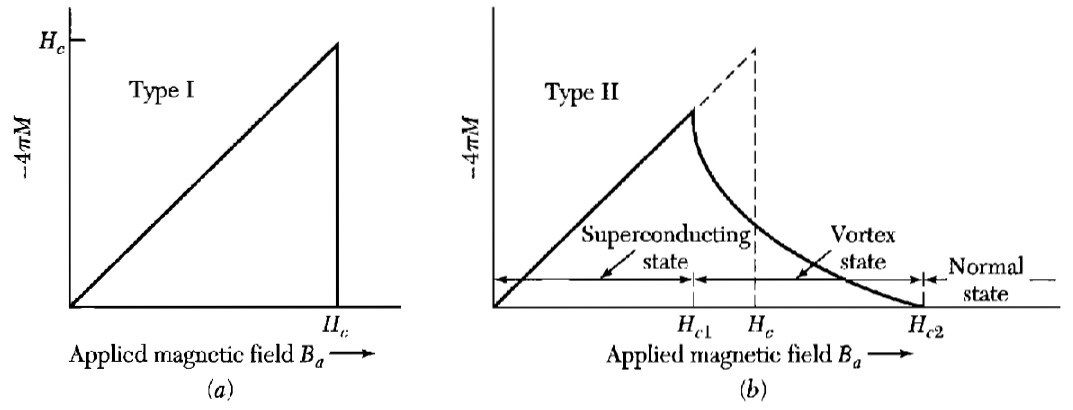
\includegraphics[width=\textwidth]{immagini/superconduttori_tipo_1_e_2.png}
   \caption*{Andamento della magnetizzazione in funzione del campo magnetico applicato per superconduttori del primo tipo (a) e del secondo tipo (b).}
\end{figure}
\hspace{-0.6cm}I materiali superconduttori del primo tipo sono quelli nei quali la lunghezza di penetrazione è più piccola della lunghezza di coerenza, viceversa nel regime opposto abbiamo i superconduttori del secondo tipo. I due tipi di superconduttori hanno una fenomenologia diversa\sn{Il fatto che si abbia una fenomenologia diversa, che stiamo per descrivere, sarà giustificato dalla teoria di Ginzburg--Landau, la quale studia situazioni in cui c'è un campo magnetico che ha una variazione nello spazio, a differenza delle teorie fenomenologiche precedenti che non hanno granché considerato la diversa risposta in queste condizioni. Essa ci permetterà di capire come tale fenomenologia nasca da essenzialmente considerazioni energetiche, cioè da come sia più conveniente da un punto di vista energetico per il materiale superconduttivo avere una penetrazione del campo magnetico con certe strutture oppure con altre.}, che è la seguente: finora abbiamo considerato superconduttori del primo tipo, che sono quelli nei quali al di sotto della temperatura critica abbiamo una risposta a un campo magnetico che è descritta dall'effetto Meissner, ovvero da un diamagnetismo perfetto, cioè se abbiamo un campo applicato $\vb{H}$, fino al valore $H_c$ abbiamo una magnetizzazione che è legata al campo applicato dalla relazione che si ha nel caso della risposta perfettamente diamagnetica, quindi abbiamo una separazione tra le due fasi con un unico valore del campo critico. I superconduttori del secondo tipo invece hanno un "diagramma di fase" un po' più articolato, nel senso che in questo caso abbiamo due valori del campo critico: un primo valore $H_{c,1}$ al di sotto del quale in effetti c'è la risposta diamagnetica con il perfetto diamagnetismo, dopo di che, superato il valore $H_{c,1}$, non si ha una risposta perfettamente diamagnetica ma non si ha nemmeno un passaggio immediato ad un comportamento normale, cioè c'è una regione di spazio in cui la relazione tra la magnetizzazione del campo critico è quella mostrata nel grafico di sopra. Nel momento in cui il sistema raggiunge un secondo valore di campo critico $H_{c,2}$, si ha il passaggio allo stato di metallo normale. In questa ragione tra i due valori di campo critico non abbiamo una perfetta espulsione del campo magnetico come abbiamo invece al di sotto di $H_{c,1}$, ma abbiamo una penetrazione del campo magnetico secondo una struttura particolare che è quella descritta da stati di vortice. Tale fatto lo possiamo vedere rappresentato qualitativamente nel seguente diagramma in funzione della temperatura e del campo magnetico:
\begin{figure}[H]
   \centering
   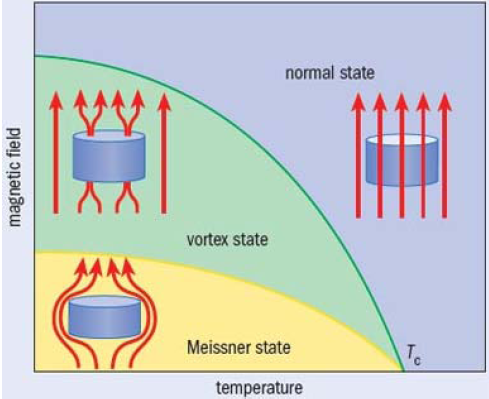
\includegraphics[width=0.6\textwidth]{immagini/grafico_T_H_superconduttori_tipo_2.png}
\end{figure}
\hspace{-0.6cm}Nel caso dei superconduttori del secondo tipo abbiamo una fase in cui abbiamo il comportamento perfettamente diamagnetico, quindi con la perfetta espulsione del campo magnetico dal materiale, una fase normale in cui invece il campo magnetico entra completamente nel materiale al di sopra della temperatura critica e una fase detta stato di vortice in cui il materiale è ancora superconductivo ma ci sono delle regioni all'interno del materiale che diventano normali le quali hanno una struttura che vede la penetrazione del campo magnetico sotto forma di vortici. Quello che cioè vedremo sono delle linee di campo magnetico che attraversano il materiale superconduttivo e a queste linee di campo magnetico che penetrano il materiale si associa una supercorrente intorno alla regione normale sotto forma di vortice, quindi una corrente che circola come se fosse intorno alla superficie di un cilindro che ha struttura\sn{credo intenda fase normale} normale. Viceversa nel regime di Meissner quello che abbiamo visto è che abbiamo una supercorrente solamente sulla superficie del materiale per una regione pari alla lunghezza di penetrazione.\sn{Man mano che il campo magnetico aumenta arrivando al campo magnetico critico quello che succede è che questa struttura di vortici diventa via via sempre più fitta fino a quando il campo magnetico penetra completamente nel materiale raggiungendo quindi lo stato normale.}
\subsection{Vortici di London}
Cerchiamo di capire più precisamente come sono fatti questi vortici. Questi in realtà possono essere già previsti dalla teoria di London e nel seguito vedremo come.\\
L'idea è rappresentata nella seguente figura:
\begin{figure}[H]
   \centering
   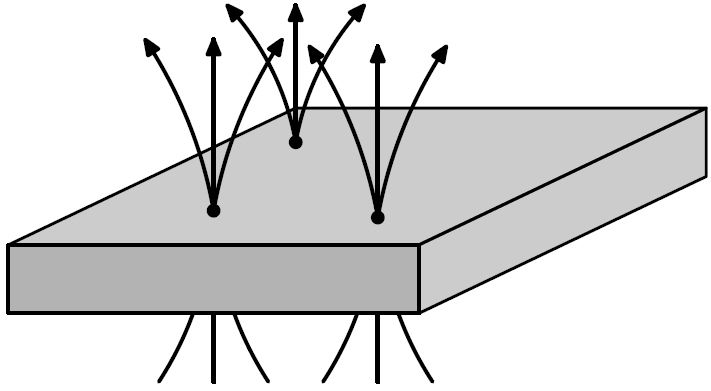
\includegraphics[width=0.5\textwidth]{immagini/vortici di London.png}
\end{figure}
\hspace{-0.6cm}Abbiamo il campo magnetico che entra all'interno del superconduttore formando un piccolo "vortex core" (in italiano "nucleo vortice") che si trova nello stato normale, quindi la regione in cui il campo magnetico penetra è una regione normale. Cerchiamo allora di capire cosa abbiamo:
\begin{figure}[H]
   \centering
   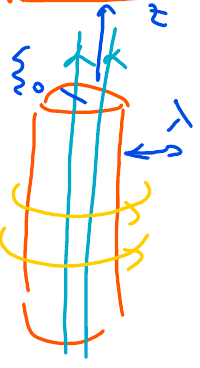
\includegraphics[width=0.2\textwidth]{immagini/vortex_core.png}
\end{figure}
\hspace{-0.6cm}Abbiamo una regione, che rappresentiamo con forma cilindrica, attraversata dal campo magnetico e il cui raggio è dell'ordine della lunghezza di coerenza. Per distanze dall'asse maggiori di $\xi_0$ ma più piccole di $\lambda$ abbiamo praticamente un superconduttore e quindi una densità di corrente $\vb{J}$ e avremo un certo campo magnetico $\vb{B}$. Possiamo ricavare questi due dall'equazione di London, la quale abbiamo visto si trasforma in un'equazione per il campo magnetico che è l'\eqrefcustom{eq:equazione_di_London_per_effetto_Meissner}, la quale, applicata ad un problema con geometria cilindrica come in questo caso e immaginando di avere un campo magnetico che è diretto lungo l'asse $z$, diventa
\begin{equation*}
   \dv[2]{B_z}{r} + \frac{1}{r} \dv{B_z}{r} - \frac{1}{\lambda^2} B_z
   =0
\end{equation*}
Tale equazione ha una soluzione nota che è espressa in termini della funzione di Bessel di ordine zero e che ha la seguente espressione:
\begin{equation*}
   B_z(r)
   =\frac{\Phi_0}{2\pi \lambda^2} K_0\qty(\frac{r}{\lambda})
\end{equation*}
dove $r$ è la distanza dall'asse e il coefficiente di proporzionalità è il flusso del campo magnetico attraverso una superficie che corrisponde alla sezione della regione normale. Quello vogliamo fare adesso a partire da questa espressione è vedere che forma assume il campo magnetico all'interno della regione di lunghezza $\lambda$ e vogliamo anche vedere com'è fatta la supercorrente. Prima di tutto consideriamo l'andamento della funzione di Bessel $K_0$, la quale quando ha argomento molto più piccolo di uno può essere approssimata nella seguente maniera:
\begin{equation*}
   K_0(z)
   \sim -\ln(z)
   \qq{se} z \ll 1
\end{equation*}
Nel nostro problema la condizione sull'argomento, visto che l'argomento di $K_0$ è $r/\lambda$, equivale a dire che $r \ll \lambda$ (ma chiaramente si deve avere comunque $r>\xi_0$, perché stiamo guardando l'equazione di London nella regione in cui il materiale è superconduttivo). In tale regione possiamo quindi riscrivere l'equazione di London come
\begin{equation}
   B_z(r)
   \sim \frac{\Phi_0}{2\pi \lambda^2} \ln\qty(\frac{\lambda}{r})
   \qq{se} \xi_0 < r \ll \lambda
   \label{eq:campo_magnetico_vortex_interno}
\end{equation}
dove abbiamo usato la proprietà del logaritmo $-\ln(z)=\ln\qty(\frac{1}{z})$.\\
Viceversa, la funzione di Bessel per argomento molto maggiore può essere approssimata come
\begin{equation*}
   K_0(z)
   \sim \sqrt{\frac{\pi}{2z}} e^{-z}
   \qq{se} z \gg 1
\end{equation*}
per cui l'equazione di London diventa
\begin{equation*}
   B_z(r)
   \sim \frac{\Phi_0}{2\pi \lambda^2} \sqrt{\frac{\pi \lambda}{2r}} e^{-r/\lambda}
   \qq{se} r \gg \lambda
\end{equation*}
La soluzione per $r \gg \lambda$ ci dà un andamento abbastanza simile, sebbene un po' più smorzato, a quello che avremmo nel caso del superconduttore di primo tipo.\\
Rivolgiamo di nuovo la nostra attenzione alla regione per valori di $r<\lambda$. In tale regione il campo magnetico ci dà una corrente che vogliamo ricavare. Per fare ciò applichiamo la legge di Ampere:
\begin{equation*}
   \oint \vb{B} \vdot \dd{\vb{l}}
   =\mu_0 \int_{\Sigma} \vb{J}_s \vdot \dd{\vb{\Sigma}}
\end{equation*}
%dove $\Sigma$ è una superficie che si appoggia sulla linea sulla quale facciamo l'integrazione. In questo caso abbiamo un campo magnetico diretto lungo l'asse $z$,
Per avere un'espressione più semplice possibile della corrente nella regione interna, scegliamo una linea di integrazione che si trova in parte nella regione in cui c'è la supercorrente, quindi per $r<\lambda$, in parte appena fuori:
\begin{figure}[H]
   \centering
   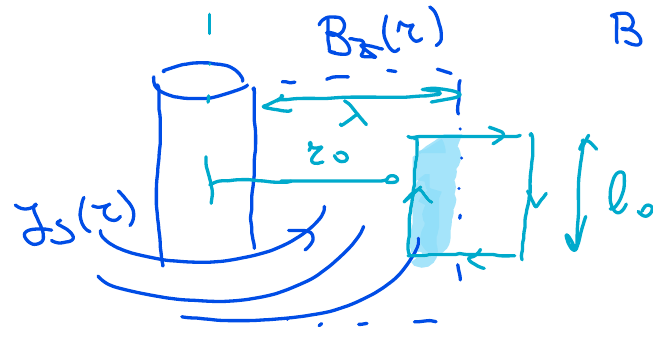
\includegraphics[width=0.5\textwidth]{immagini/cammino_di_integrazione_B_Pippard.png}
\end{figure}
\hspace{-0.6cm}Assumiamo che appena fuori (cioè per $r>\lambda$) il campo magnetico sia praticamente nullo. Se assumiamo che nella regione esterna $\vb{B}$ sia già decaduto, l'integrale di linea di $\vb{B}$ si riduce all'integrale lungo il lato interno parallelo all'asse $z$ che avrà una certa lunghezza che chiamiamo $l_0$,\mn{Il contributo negli altri due lati è zero perché essendo perpendicolari a $\vb{B}$ il prodotto scalare è nullo, il contributo lungo l'altro lato parallelo che si trova nella regione esterna è molto più piccolo e quindi trascurabile.} come mostrato nella figura precedente. In definitiva abbiamo
\begin{equation*}
   \oint \vb{B} \vdot \dd{\vb{l}}
   \approx B_z(r_0) l_0
\end{equation*}
Per la legge di Amper, esso sarà uguale al flusso della densità di corrente che passa attraverso la regione evidenziata in figura, dunque si ha
\begin{equation*}
   B_z(r) l_0
   =\mu_0 l_0 \int_{r_0}^{\lambda} J_s(r) \dd{r}
\end{equation*}
Per l'approssimazione fatta nell'\eqrefcustom{eq:campo_magnetico_vortex_interno}, sappiamo che che $B_z(r_0)$ si può esprimere come
\begin{equation*}
   B_z(r_0)
   =\frac{\Phi_0}{2\pi \lambda^2} \ln\qty(\frac{\lambda}{r_0})
\end{equation*}
quindi $\vb{J}_s$, che integrata ci deve dare il logaritmo, deve essere una funzione che va come $\frac{1}{r}$. Possiamo supporre dunque che
\begin{equation*}
   J_s(r)
   =\frac{a}{r}
\end{equation*}
Svolgendo allora i calcoli, quello che troviamo da legge di Ampere è che
\begin{equation*}
   \frac{l_0 \Phi_0}{2\pi \lambda^2} \ln\qty(\frac{\lambda}{r_0})
   =\mu_0 l_0 a \ln\qty(\frac{\lambda}{r_0})
\end{equation*}
da cui ricaviamo che
\begin{equation*}
   a
   =\frac{\Phi_0}{2\pi \mu_0 \lambda^2}
\end{equation*}
e pertanto la densità di corrente nella regione per $\xi_0 < r < \lambda$ è
\begin{equation*}
   \vb{J}_s(r)
   =\frac{\Phi_0}{2\pi \mu_0 \lambda^2} \frac{1}{r} \vu{u}_{\varphi}
   %\label{eq:densita_corrente_vortex_interno}
\end{equation*}
Cerchiamo allora di capire com'è fatto questo vortice di London:
\begin{itemize}[leftmargin=0.5cm]
   \item per $r<\xi_0$ abbiamo una regione normale in cui c'è il campo magnetico che è praticamente uniforme e pari a $\frac{\Phi_0}{\pi \xi_0^2}$;
   \item per $\xi_0 < r < \lambda$ abbiamo un campo magnetico che va come $\ln(\lambda/r)$ e una densità di corrente che va come $\frac{1}{r}$ ed è diretta a formare un vortice;
   \item per $r>\lambda$ abbiamo un decadimento esponenziale del campo magnetico.
\end{itemize}
In conclusione, la teoria di London può essere applicata anche ad un superconduttore del secondo tipo per descrivere cosa succede in corrispondenza dei vortici, che sono quelli che descrivono la penetrazione del campo magnetico nei superconductori del secondo tipo. Questa teoria di London non dice perché abbiamo questa struttura (noi siamo partiti dal supporre che ci sia questa struttura e abbiamo legato tra loro il campo magnetico e densità di corrente). La giustificazione al fatto che si ha la penetrazione del campo magnetico con queste strutture quando siamo nella condizione di superconduttore del secondo tipo ce la dirà la teoria di Ginzburg--Landau.
\subsection{Risposta AC dei superconduttori. Modello a due fluidi di Gorter e Casimir}
Fino ad ora abbiamo sostanzialmente considerato la risposta statica del campo magnetico, sebbene siamo partiti dalla conducibilità dipendente dalla frequenza in un metallo normale, abbiamo poi trattato questo metallo normale come un materiale in cui il tempo medio tra gli urti va a infinito, abbiamo approssimato la conducibilità sotto tali condizioni e poi abbiamo guardato al limite di risposta a frequenza nulla, cioè alla risposta statica.\\
In realtà nella maggior parte dei casi si ha a che fare con campi magnetici variabili nel tempo e il punto è che tutte le volte che noi abbiamo un campo magnetico variabile nel tempo la risposta del materiale non è la semplice risposta superconduttiva che abbiamo visto adesso, ma c'è anche una piccola componente di corrente dissipativà. Questo comportamento, che viene fuori anch'esso rigorosamente dalla teoria BCS, può essere descritto da una teoria basata sul nuovo modello dei due fluidi che descrive il materiale che diviene superconduttivo come un materiale che ha sia una componente normale che una componente superconduttiva, le quali hanno entrambe una risposta espressa da una conducibilità che è quella data dal modello di Drude per il materiale normale ma anche per il materiale superconduttivo, dove per il materiale superconduttivo si prende la risposta che otteniamo dall'espressione per il materiale normale mandando ad infinito il tempo medio tra gli urti. Quello che allora faremo adesso è, a partire da questo modello di due fluidi a frequenza finita, cercare di capire in quali regimi abbiamo una risposta dissipativa e in quali no, nel caso in cui abbiamo un campo variabile nel tempo.\\
Supponiamo di guardare la risposta alle differenti frequenze, dunque la risposta AC. Per inciso la teoria BCS prevede questo comportamento e lo attribuisce a effetti nati dall'eccitazione termica.\\
L'idea del modello dei due fluidi consiste nel considerare il materiale superconduttore come formato da questi due fluidi, i quali sono uno nello stato normale, quindi con la conducibilità tipica per un metallo normale, ovvero
\begin{equation*}
   \sigma_n(\omega)
   =\frac{n_n e^2 \tau_n}{m} \frac{1}{1 + i\omega \tau_n}
   =\frac{\sigma_n}{1 + i\omega \tau_n}
\end{equation*}
e uno nello stato superconduttivo che ha conducibilità avente una parte reale e una parte immaginaria che abbiamo ricavato da questo modello per $\tau \to \infty$ date da
\begin{equation*}
   \sigma_s(\omega)
   \sigma_{s,\text{Re}} - i \sigma_{s,\text{Im}}
   \approx \frac{\pi n_s e^2}{2 m} \delta(\omega) - i \frac{n_s e^2}{m \omega}
\end{equation*}
Considerare frequenze finite ma sufficientemente basse, con cui si intende considerare il regime $\omega \tau_n \ll 1$, $\tau_n$ è il tempo medio tra gli urti di un metallo normale che è dell'ordine di $10^{-12} \; \rm s$. Essendo $\omega \tau_n$ molto piccolo, possiamo appossimare la risposta del materiale normale con la sua parte reale, quindi la conducibilità totale sarà
\begin{equation*}
   \sigma(\omega)
   =\bigl[ \sigma_{s,\,\text{Re}} + \sigma_n(\omega) \bigr] - i \sigma_{s,\,\text{Im}}
   \approx \qty[ \frac{\pi n_s e^2}{2 m} \delta(\omega) + \frac{n_n e^2 \tau_n}{m}] - i \frac{n_s e^2}{m \omega}
\end{equation*}
dunque l'unico termine immaginario in questa approssimazione è quello proveniente dalla risposta del superconduttore. Sebbene questa sia una descrizione molto semplificata, essa ci dice che se guardiamo la parte reale della risposta, cioè quella che ci dà la dissipazione, essa ci dice che se siamo a frequenza nulla, dunque nel caso di risposta DC, quello che rimane è la parte reale del comportamento superconduttivo, quindi abbiamo una supercorrente e non c'è dissipazione; se invece siamo a frequenza finite diverse da zero, seppur piccole, abbiamo una risposta che ci proviene anche dalla parte normale, il quale corrisponde a un comportamento dissipativo.\\
Vediamo come capire quale dei due contributi prevale a seconda della frequenza. Supponendo che per ciascuna componente valga $\vb{J}(\omega)=\sigma(\omega)\vb{E}(\omega)$, calcoliamo il rapporto tra la componente superconduttiva e quella normale della densità di corrente. Suponendo che il campo sia lo stesso e di trovarci a frequenza finita ossia per $\omega \neq 0$,\mn{Ciò significa che resta soltanto la parte immaginaria di $\sigma_s(\omega)$, e ciò è dovuto alla presenza della $\delta(\omega)$ nella parte reale.} si trova che
\begin{equation}
   \frac{J_s(\omega)}{J_n(\omega)}
   =\frac{\sigma_{s,\text{Im}}}{\sigma_{n,\text{Re}}}
   =\frac{n_s}{n_n} \frac{1}{\omega \tau_n}
   \label{eq:rapporto_correnti_superconduttiva_normale}
\end{equation}
Tale espressione ci permette di capire che queste due correnti sono paragonabili quando
\begin{equation*}
   \omega_c
   \approx \frac{n_s}{n_n} \frac{1}{\tau_n}
\end{equation*}
Conosciamo il valore di $\tau_n$, e se supponiamo che $n_s$ e $n_n$ siano più o meno dello stesso ordine, possiamo stimare che la frequenza di crossover $\omega_c$ è dell'ordine di $10^{12} \; \rm Hz$, quindi ricade nella regione delle microonde.\\
In definitiva, l'\eqrefcustom{eq:rapporto_correnti_superconduttiva_normale} ci dice che
\begin{itemize}[leftmargin=0.5cm]
   \item se abbiamo dei campi a frequenze più basse di $\omega_c$, la componente superconduttiva della corrente prevale su quella normale, cioè $J_s(\omega)>J_n(\omega)$. Avremo comunque una componente normale, ma la risposta del materiale sarà prevalentemente superconduttiva;
   \item se abbiamo dei campi a frequenze più alte di $\omega_c$, la componente normale della corrente prevale su quella superconduttiva, cioè $J_n(\omega)>J_s(\omega)$. In questo caso avremo una risposta prevalentemente normale, con una piccola componente superconduttiva.
\end{itemize}
Questo modello a due fluidi ci permette allora di avere un'idea del range di frequenze, dunque del range di rapidità di variazione dei campi, nei quali possiamo aspettarci un comportamento superconduttivo o un comportamento normale, fermo restando che dobbiamo sempre prevedere una piccola componente dissipativa secondo.\\
In realtà, assumere che le due densità siano pressocché uguali non è sempre corretto, perché dal confronto con i risultati sperimentali sulla lunghezza di penetrazione e la sua dipendenza dalla temperatura possiamo dedurre una dipendenza dalla temperatura della densità degli elettroni superconduttivi che è proporzionare a $(T/T_c)^4$, da cui si ricava che la componente normale ha una dipendenza del tipo
\begin{equation*}
   n_n(T)
   \propto 1 - \qty(\frac{T}{T_c})^4
\end{equation*}
tale dipendenza nasce dal fatto che la somma delle due densità deve essere indipendente dalla temperatura e sia la densità complessiva degli elettroni.\\
Questi andamenti in realtà sono approssimati. La teoria BCS ci dà un andamento di tipo esponenziale che è
\begin{equation*}
   n_n(T)
   \propto e^{-\frac{\Delta}{k_B T}}
\end{equation*}
dove $\Delta$ è la gap superconduttiva. Ciò ovviamente non può venir fuori da una teoria fenomenologica perché non c'è una ragione ovvia per la quale ipotizzare che ci sia una gap energetica che separa il comportamento di questi materiali da una parte e dall'altra.
\section{Teoria di Ginzburg--Landau}
Finora abbiamo descritto la transizione superconduttiva come una transizione di fase e abbiamo visto che, a seconda della presenza o meno di un campo magnetico, essa può essere del primo o del secondo ordine. Tuttavia, non abbiamo ancora discusso in che modo una descrizione dei materiali superconduttori in termini di un potenziale termodinamico, ossia una teoria basata sulla teoria delle transizioni di fase, possa prevedere l'esistenza di queste fasi e determinarne le proprietà.\\
La teoria di Ginzburg--Landau affronta proprio questo problema. Essa si basa sull'approccio fenomenologico di Landau alle transizioni di fase e lo applica alla superconduttività, con l'obiettivo di descrivere il comportamento di un materiale metallico in presenza di un campo magnetico e di comprendere come avvenga la transizione tra la fase normale e quella superconduttiva.\\
Un aspetto essenziale della teoria è che essa tiene conto della possibilità che il campo magnetico all'interno del materiale non sia uniforme. Questo è precisamente ciò che accade nella fase superconduttiva: a causa dell'effetto Meissner, il campo magnetico viene espulso dall'interno del materiale e rimane confinato solo in determinate regioni. La teoria di Ginzburg--Landau fornisce quindi un quadro termodinamico in grado di descrivere sia la transizione di fase sia la distribuzione spaziale del campo magnetico nel materiale.
\subsection{Transizioni di fase}
L'idea è quella di considerare la fase normale e quella superconduttiva come due diverse fasi del materiale, separate da una transizione di fase. Esse possono quindi essere descritte mediante un potenziale termodinamico caratterizzato dal fatto che, nel punto di transizione, assume lo stesso valore nelle due fasi.\\
Per sviluppare questa descrizione ci basiamo sulla teoria delle transizioni di fase del secondo ordine della meccanica statistica, il cui esempio più noto è la transizione ferromagnetica. In un materiale ferromagnetico, se la temperatura è maggiore di una certa temperatura critica $T_c$, il sistema non presenta alcuna magnetizzazione macroscopica. Tuttavia, se la temperatura scende al di sotto di $T_c$, il sistema sviluppa spontaneamente una magnetizzazione in una determinata direzione.\\
Questo fenomeno avviene anche in assenza di un campo magnetico esterno ed è associato a una rottura spontanea di simmetria. Infatti, a temperature elevate il sistema non possiede una direzione privilegiata nello spazio, mentre la comparsa di una magnetizzazione spontanea introduce una direzione preferenziale. Il sistema passa quindi da uno stato più simmetrico a uno stato meno simmetrico.\\
Un comportamento analogo si ritrova nella transizione superconduttiva.\\
Per comprendere come emerga questa rottura spontanea di simmetria, consideriamo l'approccio fenomenologico proposto da Landau. In tale approccio si introduce un parametro d'ordine che caratterizza lo stato macroscopico del sistema. Nel caso del ferromagnetismo questo parametro è la magnetizzazione.\\
L'idea è quindi quella di introdurre una densità di energia libera che dipende dal parametro d'ordine. A temperature maggiori della temperatura critica questa energia libera presenta un unico minimo, che corrisponde alla configurazione con parametro d'ordine nullo. Nel caso del ferromagnetismo ciò significa che la magnetizzazione è nulla.\\
Quando invece la temperatura scende al di sotto della temperatura critica, la forma della funzione cambia: la dipendenza dell'energia libera dal parametro d'ordine passa da una struttura con un unico minimo a una struttura con due minimi degeneri corrispondenti a valori non nulli del parametro d'ordine.
\begin{figure}[H]
   \centering
   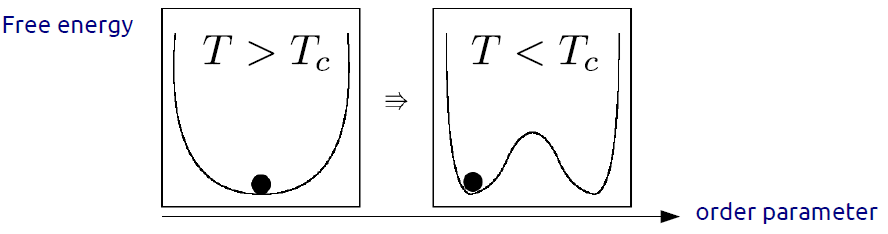
\includegraphics[width=0.9\textwidth]{immagini/andamento_energia_libera_parametro_dordine.png}
\end{figure}
\hspace{-0.6cm}Nel caso della magnetizzazione ciò significa che, al di sotto della temperatura critica, il sistema sceglie spontaneamente una delle configurazioni di energia minima, corrispondente a una magnetizzazione diversa da zero orientata in una certa direzione.\\
Il parametro $\psi$ che descrive questo cambiamento dello stato del sistema è detto parametro d'ordine. Nel caso del ferromagnetismo esso può essere identificato con la magnetizzazione, che è nulla per $T>T_c$ e diversa da zero per $T<T_c$.\\
Parliamo ora in termini più generali della teoria di Landau delle transizioni di fase. Introduciamo un parametro d'ordine $\psi$.\mn{Nella teoria di Ginzburg--Landau esso è un oggetto complesso; per il momento possiamo tuttavia considerarlo reale. Nel caso del ferromagnetismo esso corrisponde al modulo della magnetizzazione, $|\vb{M}|$.}\\
La teoria di Landau consiste nello scrivere la densità di energia libera come funzione del parametro d'ordine. Nel caso della superconduttività si può scrivere
\begin{equation}
   f_s = f_n + a |\psi|^2 + \frac{b}{2} |\psi|^4
   \label{eq:energia_libera_Ginzburg_Landau}
\end{equation}
dove $f_n$ è la densità di energia libera della fase normale e gli altri termini rappresentano il contributo associato allo stato superconduttivo.\\
L'idea alla base della teoria delle transizioni di fase del secondo ordine è quella di sviluppare l'energia libera della nuova fase in serie di Taylor rispetto al parametro d'ordine intorno allo stato normale. Si includono i termini quadratici e quartici perché questa è la struttura più semplice che permetta di descrivere la comparsa di nuovi minimi dell'energia libera.\\
In particolare, il coefficiente $b$ rimane positivo, mentre il coefficiente $a$ dipende dalla temperatura secondo la legge
\begin{equation*}
   a(T) = a' \frac{T-T_c}{T_c},
   \qq{con} a' > 0
\end{equation*}
In questo modo $a$ risulta positivo per $T>T_c$ e negativo per $T<T_c$.
\begin{figure}[H]
   \centering
   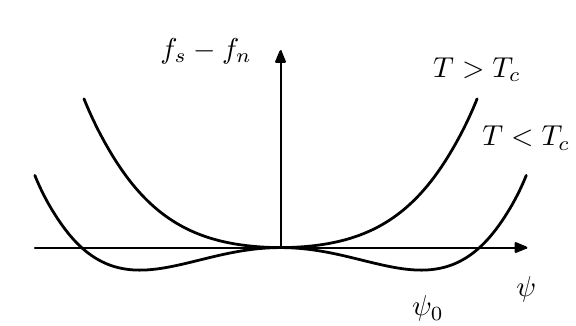
\includegraphics[width=0.6\textwidth]{immagini/differenze_energie_libere.png}
\end{figure}
\hspace{-0.6cm}Se $T>T_c$, la differenza tra le densità di energia libera delle due fasi presenta un unico minimo in corrispondenza di $\psi=0$, che corrisponde alla fase normale.\\
Se invece $T<T_c$, il coefficiente $a$ diventa negativo e la funzione assume la tipica forma a doppia buca. I minimi si trovano per valori non nulli del parametro d'ordine. Per determinarli calcoliamo i valori in corrispondenza dei quali la differenza tra le energie libere delle due fasi è minima, ossia calcoliamo i punti in cui la derivata rispetto a $|\psi|$ si annulla:
\begin{equation*}
   \dv{(f_s - f_n)}{|\psi|}
   =2a |\psi| + 2b |\psi|^3 =0
\end{equation*}
Da questa relazione otteniamo
\begin{equation*}
   |\psi_{\rm min}|^2 = -\frac{a}{b} > 0
\end{equation*}
che è positivo perché $a<0$ per $T<T_c$.\\
Sostituendo l'espressione di $a(T)$ si trova
\begin{equation*}
   \psi_{\rm min}
   =\sqrt{\frac{a'(T_c-T)}{b T_c}}
\end{equation*}
Infine, sostituendo questo valore nell'energia libera si ottiene
\begin{equation*}
   f_s
   = f_n - \frac{{a'}^2}{2b} \qty(\frac{T_c-T}{T_c})^2
\end{equation*}
Da questa espressione si vede che per $T<T_c$ la fase superconduttiva ha energia libera più bassa rispetto alla fase normale ed è quindi termodinamicamente stabile, mentre per $T>T_c$ è stabile la fase normale.
\subsection{Teoria di Ginzburg--Landau per la superconduttività}
L'idea è quella di descrivere la transizione dalla fase normale alla fase superconduttiva di un metallo come una transizione di fase. Per farlo consideriamo una descrizione termodinamica del materiale. In altre parole, per descrivere la transizione di fase dobbiamo introdurre un'energia libera che descriva il sistema che stiamo studiando, identificando quali sono i parametri rilevanti che guidano la transizione. In questo caso tali parametri sono in particolare la temperatura e il campo magnetico. Sappiamo infatti che la transizione dalla fase normale alla fase superconduttiva avviene diminuendo la temperatura; essa è quindi uno dei parametri che possiamo variare per indurre la transizione. L'altro parametro è il campo magnetico, poiché sappiamo che la transizione può avvenire solo se il campo magnetico è inferiore a un certo campo critico che dipende dalla temperatura.\\
L'idea è quindi quella di considerare queste due fasi come diverse fasi termodinamiche del metallo, separate da una transizione di fase. L'evidenza della transizione di fase si manifesta nelle grandezze termodinamiche, in particolare nel calore specifico del superconduttore, come vedremo più avanti.\\
Applichiamo ora la teoria di Ginzburg--Landau alla transizione dalla fase normale alla fase superconduttiva e dobbiamo identificare il parametro d'ordine appropriato $\psi$. Questa teoria fu sviluppata nel 1950 ed è estremamente ingegnosa, nel senso che a quel tempo non si conosceva ancora il meccanismo microscopico responsabile della superconduttività. Tuttavia si intuiva già che il fenomeno dovesse avere un'origine quantistica. L'idea era quindi che la superconduttività fosse un fenomeno di natura quantomeccanica, pur non conoscendo ancora il motivo preciso per cui si verificasse, e che mostrasse una transizione di fase analoga a quelle note nei sistemi classici.\\
Si cercò quindi di identificare un parametro d'ordine che descrivesse le configurazioni macroscopiche stabili del sistema. Tenendo presente la natura quantistica del fenomeno, si assunse che il parametro d'ordine fosse una quantità complessa $\psi$, con l'idea che potesse svolgere il ruolo di una funzione d'onda che descrive la fase superconduttiva. In altre parole, si utilizzò come parametro d'ordine una quantità che, in qualche modo, potesse essere interpretata come una funzione d'onda macroscopica del sistema.\mn{A questo livello, per funzione d'onda si intende semplicemente un parametro d'ordine complesso.}\\
Questa intuizione era anche influenzata dagli sviluppi teorici relativi alla superfluidità dell'elio $^4\mathrm{He}$. Infatti la teoria della superfluidità era stata sviluppata prima di quella della superconduttività, e in quel contesto era stata introdotta una funzione d'onda macroscopica per descrivere il fluido superfluido. L'idea di una funzione d'onda macroscopica per il superconduttore fu quindi ispirata anche da questi risultati.\\
Circa dieci anni più tardi fu possibile dimostrare che il parametro d'ordine della teoria di Ginzburg--Landau è effettivamente legato alla densità locale dei portatori di carica nel superconduttore. In particolare si trovò che $|\psi|^2$ è proporzionale alla densità degli elettroni superconduttivi.\\
Cominciamo quindi scrivendo la densità di energia libera $f$ in funzione del parametro d'ordine complesso. L'energia libera che utilizziamo è l'energia libera di Gibbs, poiché abbiamo visto che essa è il potenziale termodinamico appropriato per descrivere una transizione guidata da variazioni di temperatura e di campo magnetico applicato $H$.\\
Vogliamo quindi scrivere l'energia libera di Gibbs della fase superconduttiva come funzione dell'energia libera della fase normale più alcuni contributi che dipendono dal parametro d'ordine $\psi$. In altre parole, ci aspettiamo che l'energia libera sia una funzione del parametro d'ordine.\\
Per determinare la forma di questa dipendenza consideriamo le seguenti ipotesi:
\begin{itemize}[leftmargin=0.5cm]
   \item $f_s$ deve coincidere con l'energia libera della fase normale $f_n$ quando il parametro d'ordine tende a zero, cioè quando $\psi \to 0$ (per semplicità, per il momento supponiamo $\psi$ reale);
   \item Sappiamo che la transizione avviene modificando la temperatura, quindi possiamo supporre che $f_s$ sia dato da $f_n$ più un contributo che dipende almeno dalla temperatura (per il momento trascuriamo il campo magnetico);
   \item La differenza $f_s - f_n$, considerata come funzione di $\psi$, deve essere una funzione simmetrica che per $T>T_c$ possiede un unico minimo stabile in $\psi=0$ (quindi deve avere una forma parabolica), mentre per $T<T_c$ deve presentare una rottura di simmetria, cioè una funzione simmetrica con minimi per valori di $\psi$ diversi da zero. Inoltre la forma della funzione deve cambiare in modo continuo al variare della temperatura.
\end{itemize}
La funzione più semplice che possiede queste proprietà può essere ottenuta sviluppando la densità di energia libera in serie di Taylor attorno allo stato normale. Per ottenere un comportamento parabolico è necessario un termine quadratico, quindi il primo contributo può essere scritto nella forma $a\psi^2$, dove $a$ è una funzione della temperatura tale che il potenziale abbia la forma desiderata. In particolare $a$ deve essere proporzionale a $T-T_c$, in modo da risultare positivo per $T>T_c$.\\
Quando la temperatura scende al di sotto di $T_c$, la differenza $f_s - f_n$ deve invece assumere la forma a doppia buca mostrata in precedenza. Per ottenere questo comportamento è necessario aggiungere un termine quartico $b\psi^4$.\\
Il coefficiente $b$ deve essere positivo affinché il sistema abbia una fase stabile per $\psi=0$ quando $T>T_c$. Quando invece $T<T_c$, il sistema avrà una fase stabile con un valore non nullo di $\psi$.\\
Vediamo più precisamente come emerge questa struttura. Il minimo di $f_s - f_n$ si trova imponendo
\begin{equation*}
   \dv{(f_s-f_n)}{\psi}
   =2a\psi + 2b\psi^3
   =2\psi(a+b\psi^2)
   =0
\end{equation*}
da cui segue che o $\psi=0$ oppure
\begin{equation*}
   \psi^2=-\frac{a}{b}
\end{equation*}
Poiché $\psi^2$ deve essere positivo, questa soluzione è possibile solo quando $a<0$. Scrivendo
\begin{equation*}
   a(T)=a'\frac{T-T_c}{T_c}
\end{equation*}
si ottiene
\begin{equation*}
   \psi^2
   =-\frac{a'}{b}\frac{T-T_c}{T_c}
\end{equation*}
che è positivo solo per $T<T_c$.\\
Questo significa che per $T>T_c$ il minimo si trova in $\psi=0$, cioè le energie libere delle due fasi coincidono e la fase stabile è quella normale. Per $T<T_c$, invece, la soluzione stabile corrisponde a un valore non nullo del parametro d'ordine.\\
Sostituendo questo valore nell'energia libera si ottiene
\begin{equation}
   f_s
   =f_n - \frac{{a'}^2}{2b}\left(\frac{T_c-T}{T_c}\right)^2
   \label{eq:free_energy_ginzburg_landau}
\end{equation}
La relazione \eqrefcustom{eq:free_energy_ginzburg_landau} mostra che la densità di energia libera della fase superconduttiva è minore di quella della fase normale quando $T<T_c$, e quindi la fase stabile è quella superconduttiva.\\
In questo modo, applicando la teoria di Landau delle transizioni di fase del secondo ordine, riusciamo a descrivere in modo fenomenologico il comportamento dei superconduttori che subiscono una transizione di fase a campo magnetico nullo quando $T<T_c$.\\
C'è però un aspetto importante da ricordare. Finora abbiamo introdotto il parametro d'ordine complesso come un'intuizione basata sulla natura quantistica del fenomeno. Il fatto che il parametro sia complesso implica che possiamo scriverlo nella forma\\
\begin{equation*}
   \psi = |\psi| e^{i\vartheta}
\end{equation*}
Osserviamo però che l'energia libera dipende solo da $|\psi|^2$, quindi non dipende dalla fase $\vartheta$, ma soltanto dall'ampiezza.\\
Questo significa che, quando avviene la transizione alla fase superconduttiva, il parametro d'ordine assume un valore
\begin{equation*}
   \psi_s = |\psi_s| e^{i\vartheta_s}
\end{equation*}
dove $|\psi_s|$ è determinato dalla condizione di minimo dell'energia libera, mentre la fase $\vartheta_s$ può assumere un valore arbitrario.\\
Anche se la fase non compare esplicitamente nell'energia libera, essa esiste nel parametro d'ordine che descrive la fase superconduttiva. Di conseguenza, quando avviene la transizione il sistema deve scegliere spontaneamente un valore della fase.\\
Questo è, in una certa misura, analogo a ciò che accade nella transizione ferromagnetica: in quel caso il sistema sceglie spontaneamente una direzione della magnetizzazione. Nel caso della transizione superconduttiva, invece, il sistema sceglie spontaneamente una fase. Vedremo più avanti che questa fase ha un significato fisico molto importante, nonostante in meccanica quantistica siamo spesso abituati a considerare la fase della funzione d'onda come non rilevante.
\subsection{Proprietà termodinamiche}
La prima cosa che dobbiamo verificare è se la dipendenza dell'energia libera dalla temperatura, data dall'\eqrefcustom{eq:free_energy_ginzburg_landau}, sia in grado di descrivere le proprietà termodinamiche dei superconduttori, e in particolare il calore specifico.
\begin{figure}[H]
   \centering
   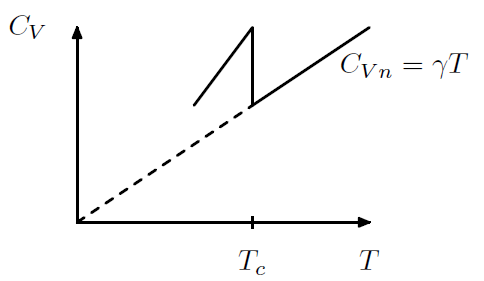
\includegraphics[width=0.6\textwidth]{immagini/calore_specifico_ginzburg_landau.png}
   \caption*{Calore specifico di un superconduttore in prossimità di $T_c$ nel modello di Ginzburg--Landau. Al di sopra di $T_c$ il calore specifico è quello previsto dalla teoria di Sommerfeld dei metalli, $C_{V,n}=\gamma T$. In corrispondenza di $T_c$ si osserva una discontinuità e un cambiamento della pendenza.}
\end{figure}
\hspace{-0.6cm}Abbiamo visto che una delle evidenze della transizione alla fase superconduttiva si manifesta anche nelle proprietà termodinamiche. In particolare, osservando l'andamento del calore specifico in funzione della temperatura, si nota che per $T>T_c$ il sistema presenta la tipica dipendenza lineare dalla temperatura, che corrisponde al comportamento normale dei metalli. Per temperature inferiori a $T_c$ (e in particolare in corrispondenza di $T=T_c$) si osserva invece una discontinuità nel calore specifico.\\
Questa discontinuità è un'indicazione della presenza di una transizione di fase e costituisce quindi una evidenza termodinamica della transizione superconduttiva.\\
Avendo a disposizione un'espressione per l'energia libera, possiamo derivarne il calore specifico e verificare se la dipendenza dalla temperatura che abbiamo ottenuto è in grado di descrivere questo salto nel calore specifico.\\
Abbiamo visto, attraverso l'\eqrefcustom{eq:relazione_termodinamica_campo_critico}, che la differenza tra le energie libere delle due fasi è anche legata alla densità di energia magnetica. In particolare, quando il campo magnetico applicato è uguale al campo critico alla temperatura considerata, vale la relazione
\begin{equation*}
   f_s(T,H_c)
   - f_n(T,H_c)
   =-\frac{H_c^2(T)}{8\pi}
\end{equation*}
Consideriamo ora il calore specifico. Per calcolarlo dobbiamo studiare la variazione dell'energia libera, cioè $\dd f$. Poiché l'energia libera dipende dalla temperatura e dal campo magnetico, $f=f(T,B)$, la sua variazione è data da
\begin{equation*}
   \dd{f}
   = -s\,\dd{T} + \frac{H}{4\pi} \dd{B}
\end{equation*}
Da questa relazione si vede immediatamente che il calore specifico è dato da
\begin{equation*}
   C
   =T\qty(\pdv{s}{T})_B
   =-T\qty(\pdv[2]{f}{T})_B
\end{equation*}
Ciò significa che, per determinare il calore specifico del superconduttore utilizzando l'\eqrefcustom{eq:free_energy_ginzburg_landau}, è sufficiente calcolare la derivata seconda dell'energia libera rispetto alla temperatura e moltiplicarla per $T$. Si ottiene così
\begin{equation*}
   C_s - C_n
   =- T \pdv[2]{T}
   \qty[ -\frac{{a'}^2}{2b} \qty(\frac{T_c-T}{T_c})^2 ]
   =- \frac{{a'}^2}{b}\frac{T}{T_c^2}
\end{equation*}
La differenza tra il calore specifico nella fase superconduttiva e quello nella fase normale alla temperatura critica risulta quindi
\begin{equation*}
   \bigl[ C_s - C_n \bigr]_{T=T_c}
   =\frac{{a'}^2}{b}\frac{1}{T_c}
\end{equation*}
il che mostra esplicitamente la presenza di un salto nel calore specifico in corrispondenza della temperatura critica.
\subsection{Sistemi non omogenei}
Finora abbiamo considerato $\psi$ come un parametro d'ordine uniforme. In realtà, la teoria di Ginzburg--Landau è in grado di descrivere anche variazioni spaziali della fase superconduttiva. Essa può quindi descrivere situazioni in cui il sistema presenta regioni che sono superconduttive e regioni che non lo sono.\\
Abbiamo già incontrato un esempio semplice di questa situazione quando abbiamo considerato il caso idealizzato di un superconduttore che occupa un semispazio, con il vuoto dall'altra parte. In quel caso abbiamo visto che il campo magnetico penetra nel materiale per una certa distanza dalla superficie. In prossimità della superficie è presente una corrente schermante e può esistere una regione del materiale che non è completamente nello stato superconduttivo, mentre più all'interno il materiale è pienamente superconduttivo.\\
Anche in situazioni molto semplici è quindi necessario poter descrivere un sistema che presenta regioni normali e regioni superconduttive.\\
Per farlo, in questa teoria dobbiamo introdurre un parametro d'ordine complesso che varia nello spazio. Questo è uno dei punti di forza della teoria di Ginzburg--Landau: essa è in grado di descrivere correttamente situazioni in cui il parametro d'ordine cambia nello spazio, purché ci si trovi a temperature vicine alla temperatura critica.\\
L'idea è quindi che il parametro d'ordine diventa una funzione della posizione. Pertanto, esso avrà sia un'ampiezza sia una fase che dipendono dalla posizione:
\begin{equation*}
   \psi
   \equiv \psi(\vb{r})
   = |\psi(\vb{r})| e^{i\vartheta(\vb{r})}
\end{equation*}
La domanda è quindi come questa dipendenza dalla posizione entri nell'espressione dell'energia libera. L'intuizione è la seguente: se immaginiamo che questa funzione descriva l'intero superconduttore, cioè lo stato macroscopico formato da un grandissimo numero di elettroni, allora possiamo identificare il modulo quadro di questa quantità, $|\psi(\vb{r})|^2$, con la densità locale di elettroni superconduttivi.\\
Questa idea è ispirata dall'analogia con la meccanica quantistica. Infatti, se $\psi$ è la funzione d'onda di una singola particella, allora $|\psi|^2$ rappresenta la densità di probabilità di trovare la particella nello spazio. Se invece immaginiamo di avere una funzione d'onda macroscopica che descrive il condensato superconduttivo, è naturale interpretare il modulo quadro di tale funzione come la densità locale degli elettroni superconduttivi.\\
Se adottiamo questa interpretazione e pensiamo all'energia libera del superconduttore come alla somma di tutti i contributi energetici rilevanti, è naturale includere nell'energia libera un termine che ricordi l'energia cinetica di una particella.\mn{\cite{Annett} Ginzburg e Landau postularono che l'energia libera avesse la forma dell'\eqrefcustom{eq:energia_libera_Ginzburg_Landau}, a cui si aggiunge un nuovo termine dipendente dal gradiente di $\psi(\vb{r})$.}\\
Seguendo questa prospettiva, dobbiamo quindi introdurre un termine che dipenda dal gradiente di $\psi$. In meccanica quantistica, infatti, l'energia di una particella libera è $\frac{\vb{p}^2}{2m}$ e l'operatore impulso è legato al gradiente della funzione d'onda.\\
L'idea è quindi che, per descrivere situazioni in cui il parametro d'ordine varia nello spazio, si debba includere nell'espressione della densità di energia libera del superconduttore un termine analogo a un contributo di energia cinetica. Si ottiene così
\begin{equation}
   f_s(\vb{r})
   = f_n
   + \frac{\hbar^2}{2m^*} |\grad{\psi}|^2
   + a(T) |\psi|^2
   + \frac{b(T)}{2} |\psi|^4
   \label{eq:free_energy_ginzburg_landau_inhomogeneous}
\end{equation}
Notiamo che abbiamo introdotto una massa $m^*$, che rappresenta la massa efficace dei portatori di carica nel superconduttore. All'epoca della formulazione della teoria non era possibile determinarne il valore. Vedremo in seguito che questa massa efficace corrisponde in realtà alla massa di due elettroni.\\
Questo termine può essere compreso anche da un punto di vista più matematico, considerando nuovamente l'energia libera come una sorta di espansione in serie di Taylor. Se infatti il parametro d'ordine dipende da un'altra variabile, in particolare dalla posizione, è naturale che compaiano contributi aggiuntivi legati alle derivate spaziali di $\psi$, cioè al gradiente di $\psi$.
\subsection{Derivazione delle equazioni di Ginzburg--Landau}
Il nostro obiettivo è ora determinare la funzione $\psi(\vb{r})$ che minimizza l'energia libera. La situazione è più complessa rispetto al caso precedente, in cui avevamo semplicemente un potenziale a doppia buca, poiché ora il parametro d'ordine può variare nello spazio.\\
Possiamo scrivere l'energia libera come integrale nello spazio della densità di energia libera. In questo modo l'espressione \eqrefcustom{eq:free_energy_ginzburg_landau_inhomogeneous} diventa
\begin{equation}
   F_s(T)
   = F_n(T) + \int \dd[3]{\vb{r}} \qty(
   \frac{\hbar^2}{2m^*} |\grad{\psi}|^2
   + a(T) |\psi(\vb{r})|^2
   + \frac{b(T)}{2} |\psi(\vb{r})|^4
   )
   \label{eq:differenza_energie_libere_integrata}
\end{equation}
Per trovare la funzione $\psi(\vb{r})$ che minimizza l'energia libera utilizziamo un approccio variazionale. Consideriamo quindi una variazione infinitesima del parametro d'ordine:
\begin{equation}
   \psi(\vb{r})
   \to \psi(\vb{r}) + \delta \psi(\vb{r})
   \label{eq:variazione_parametro_dordine}
\end{equation}
e calcoliamo la variazione dell'energia libera al primo ordine in $\delta\psi$. La condizione di minimo richiede che tale variazione sia nulla.\\
Sostituendo $\psi$ e $\psi^*$ nella forma dell'\eqrefcustom{eq:variazione_parametro_dordine} all'interno dell'\eqrefcustom{eq:differenza_energie_libere_integrata} e mantenendo solo i termini al primo ordine in $\delta\psi$ e $\delta\psi^*$, si ottiene
\begin{equation*}
   \begin{split}
      \delta F_s
      &= \int \dd[3]{\vb{r}} \qty[
      \frac{\hbar^2}{2m^*} (\grad{\delta \psi^*}) \cdot (\grad{\psi})
      + \delta \psi^* \qty( a\psi + b \psi |\psi|^2 )
      ]
      \\
      &\quad + \int \dd[3]{\vb{r}} \qty[
      \frac{\hbar^2}{2m^*} (\grad{\psi^*}) \cdot (\grad{\delta \psi})
      + \delta \psi \qty( a\psi^* + b \psi^* |\psi|^2 )
      ]
   \end{split}
\end{equation*}
Il passo successivo consiste nel semplificare queste espressioni mediante integrazione per parti. Trascurando i termini di superficie (assumendo condizioni al contorno appropriate), si ottiene
\begin{equation}
\begin{split}
   \delta F_s
   &= \int \dd[3]{\vb{r}} \,
   \delta \psi^* \qty(
   -\frac{\hbar^2}{2m^*} \laplacian{\psi}
   + a\psi + b\psi |\psi|^2
   )
   \\
   &\quad + \int \dd[3]{\vb{r}} \,
   \delta \psi \qty(
   -\frac{\hbar^2}{2m^*} \laplacian{\psi}
   + a\psi + b\psi |\psi|^2
   )^*
\end{split}
\label{eq:variazione_energia_libera_ginzburg_landau}
\end{equation}
Imponendo la condizione di minimo $\delta F_s = 0$, e osservando che i due termini sono complessi coniugati tra loro, si ottiene la condizione
\begin{equation}
   -\frac{\hbar^2}{2m^*} \laplacian{\psi(\vb{r})}
   + \qty(a + b |\psi(\vb{r})|^2)\psi(\vb{r})
   = 0
   \label{eq:ginzburg_landau_equation_no_magnetic_field}
\end{equation}
che prende il nome di \emph{equazione di Ginzburg--Landau} (in assenza di campo magnetico).\\
Questa equazione determina il valore spaziale del parametro d'ordine $\psi(\vb{r})$. Dal punto di vista formale, essa ha una struttura simile all'equazione di Schrödinger, ma presenta un termine non lineare, $b|\psi|^2\psi$, che è proprio il contributo responsabile della transizione di fase.
\subsection{Derivazione alternativa delle equazioni di Ginzburg--Landau}
L'\eqrefcustom{eq:ginzburg_landau_equation_no_magnetic_field} può essere ottenuta anche in modo più formale, considerando l'energia libera come un funzionale della funzione parametro d'ordine:
\begin{equation*}
   F_s[\psi]
   = \int \dd[3]{\vb{r}} \, f_s(\vb{r})
\end{equation*}
In questo caso, la variazione dell'energia libera può essere espressa in termini di derivate funzionali come
\begin{equation*}
   \delta F_s
   = \int \dd[3]{\vb{r}} \qty[
   \pdv{F_s[\psi]}{\psi(\vb{r})}\,\delta \psi(\vb{r})
   + \pdv{F_s[\psi]}{\psi^*(\vb{r})}\,\delta \psi^*(\vb{r})
   ]
\end{equation*}
Le derivate funzionali possono essere calcolate esplicitamente a partire dall'espressione dell'energia libera, oppure, poiché abbiamo già svolto la derivazione variazionale, possono essere identificate confrontando questa espressione con l'\eqrefcustom{eq:variazione_energia_libera_ginzburg_landau}. Si ottiene così
\begin{equation*}
   \begin{dcases}
      \pdv{F_s[\psi]}{\psi^*(\vb{r})}
      = -\frac{\hbar^2}{2m^*}\laplacian{\psi}
      + a(T)\psi + b(T)\psi |\psi|^2
      \\
      \pdv{F_s[\psi]}{\psi(\vb{r})}
      = \qty(
      -\frac{\hbar^2}{2m^*}\laplacian{\psi}
      + a(T)\psi + b(T)\psi |\psi|^2
      )^*
   \end{dcases}
\end{equation*}
Imponendo la condizione di minimo $\delta F_s = 0$, si deve richiedere che entrambe le derivate funzionali si annullino:
\begin{equation*}
   \pdv{F_s[\psi]}{\psi(\vb{r})} = 0
   \qq{,}
   \pdv{F_s[\psi]}{\psi^*(\vb{r})} = 0
\end{equation*}
Queste condizioni conducono nuovamente all'equazione di Ginzburg--Landau \eqrefcustom{eq:ginzburg_landau_equation_no_magnetic_field}.
\subsection{Sistemi non omogenei in presenza di campo magnetico}
Finora abbiamo considerato la transizione di fase in assenza di campo magnetico applicato. Tuttavia, sappiamo che la superconduttività è un fenomeno che si manifesta anche in presenza di un campo magnetico, ed è quindi necessario includere i suoi effetti nella teoria.\\
Vediamo dunque come introdurre il campo magnetico nell'espressione dell'energia libera. Ginzburg e Landau postularono che il campo magnetico entri nella teoria come se $\psi(\vb{r})$ fosse la funzione d'onda di particelle cariche, cioè attraverso la sostituzione standard della meccanica quantistica
\begin{equation*}
   \frac{\hbar}{i}\grad
   \;\to\;
   \frac{\hbar}{i}\grad - \frac{e^*}{c}\vb{A}
\end{equation*}
dove $\vb{A}$ è il potenziale vettore.\\
È inoltre necessario includere nell'energia libera un contributo associato all'energia del campo magnetico. Questo perché l'energia libera descrive l'intero campione, che può contenere anche regioni non completamente superconduttive in cui il campo magnetico è presente.\\
La densità di energia libera diventa quindi\mn{Dalla teoria BCS si trova che $m^* = 2m$ ed $e^* = -2e$.}
\begin{equation*}
   f_s(\vb{r})
   = f_n
   + \frac{1}{2m^*}
   \abs{ \qty( \frac{\hbar}{i}\grad - \frac{e^*}{c}\vb{A} ) \psi }^2
   + a |\psi|^2
   + \frac{b}{2} |\psi|^4
   + \frac{h^2}{8\pi}
\end{equation*}
dove $h$ è il campo magnetico locale.\\
Come nel caso precedente, il passo successivo è determinare la funzione $\psi(\vb{r})$ che minimizza l'energia libera. Tuttavia, in questo caso la situazione è più complessa, poiché l'energia libera dipende non solo da $\psi$ e $\psi^*$, ma anche dal potenziale vettore $\vb{A}$ e quindi dal campo magnetico.\\
È quindi conveniente utilizzare un approccio variazionale più generale, trattando sia $\psi$ sia $\vb{A}$ come variabili indipendenti e scrivendo le corrispondenti equazioni di Eulero--Lagrange.\\
Da questa procedura si ottengono due equazioni. La prima equazione di Ginzburg--Landau è
\begin{equation}
   a\psi + b |\psi|^2 \psi
   + \frac{1}{2m^*}
   \qty(
   \frac{\hbar}{i}\grad - \frac{e^*}{c}\vb{A}
   )^2 \psi
   = 0
   \label{eq:1_GL_equation_with_magnetic_field}
\end{equation}
Questa equazione ha la struttura di un'equazione di Schrödinger non lineare, in cui il termine cinetico è reso gauge invariante mediante la sostituzione del momento con il momento canonico accoppiato al campo elettromagnetico.\\
La seconda equazione si ottiene variando l'energia libera rispetto al potenziale vettore $\vb{A}$. Essa descrive l'origine del campo magnetico all'interno del superconduttore, che può essere generato soltanto da una corrente. Nel caso superconduttivo, tale corrente è una supercorrente.\\
Si ottiene quindi una relazione equivalente alla legge di Ampère:
\begin{equation*}
   \curl{\vb{h}}
   = \frac{4\pi}{c} \vb{J}_s
\end{equation*}
La densità di supercorrente è data da
\begin{equation*}
   \vb{J}_s
   = - \pdv{f_s}{\vb{A}(\vb{r})}
\end{equation*}
Svolgendo il calcolo esplicito si trova
\begin{equation*}
   \vb{J}_s
   = \frac{e^*\hbar}{2m^* i}
   \qty[
   \psi^* \qty( \grad - \frac{ie^*}{\hbar c}\vb{A} ) \psi
   - \qty( \grad + \frac{ie^*}{\hbar c}\vb{A} ) \psi^* \psi
   ]
\end{equation*}
Riordinando i termini, questa espressione può essere scritta come
\begin{equation*}
   \vb{J}_s
   = \vb{J}_{h=0}
   - \frac{{e^*}^2}{m^* c} |\psi|^2 \vb{A}
\end{equation*}
dove $\vb{J}_{h=0}$ rappresenta la corrente in assenza di campo magnetico.\\
Cerchiamo ora di interpretare il significato delle equazioni ottenute. Abbiamo scritto un'energia libera che include anche il contributo dell'energia magnetica, e dalla sua minimizzazione otteniamo le condizioni sia per il parametro d'ordine $\psi$ sia per le proprietà magnetiche del sistema.\\
Se in un materiale, sia esso un metallo normale o un superconduttore, è presente un campo magnetico, allora deve esserci una corrente che lo genera. Non è quindi sorprendente che dalla minimizzazione dell'energia libera emerga una relazione equivalente alla legge di Ampère per una densità di supercorrente.\\
Questa densità di corrente può essere separata in due contributi: una parte $\vb{J}_{h=0}$ presente anche in assenza di campo magnetico e un termine addizionale che compare in presenza del campo magnetico, cioè del potenziale vettore $\vb{A}$.\\
Consideriamo innanzitutto il termine presente anche in assenza di campo magnetico. In questo caso, l'espressione della densità di supercorrente coincide formalmente con quella della corrente associata a una particella descritta da una funzione d'onda $\psi$:
\begin{equation*}
   \vb{J}_{h=0}
   = \frac{e^* \hbar}{2m^* i}
   \qty( \psi^* \grad{\psi} - \psi \grad{\psi^*} )
\end{equation*}
Questa è la ben nota espressione della corrente di probabilità in meccanica quantistica. Essa può essere intuita osservando che, se $|\psi|^2$ rappresenta la densità dei portatori, allora la densità di corrente si ottiene combinando tale densità con l'operatore impulso, che è proporzionale al gradiente.\\
Nel caso di una particella singola, in presenza di un campo magnetico, questa espressione si modifica esattamente nello stesso modo in cui si modifica l'impulso, cioè mediante il principio di sostituzione minimale. Lo stesso avviene qui: in presenza di campo magnetico compare un termine aggiuntivo nella corrente.\\
Possiamo quindi separare la densità di corrente in una parte a campo nullo e una parte proporzionale al potenziale vettore $\vb{A}$. Se identifichiamo $|\psi|^2$ con la densità dei portatori superconduttivi $n_s$, nel caso omogeneo in cui $\grad{\psi}=0$ otteniamo
\begin{equation*}
   \vb{J}
   = - \frac{{e^*}^2}{m^* c} n_s \vb{A}
\end{equation*}
che coincide con l'equazione di London.\\
Consideriamo ora il caso non omogeneo, in cui $\psi$ varia nello spazio. Il parametro d'ordine sarà quindi nella forma
\begin{equation}
   \psi(\vb{r}) = |\psi(\vb{r})| e^{i\phi(\vb{r})}
   \label{eq:psi_con_fase}
\end{equation}
Poiché si ha
\begin{equation*}
   \grad{\psi}
   = e^{i\phi} \qty( \grad{|\psi|} + i |\psi| \grad{\phi} )
\end{equation*}
possiamo riscrivere la densità di corrente come
\begin{equation}
   \vb{J}_s
   = \frac{e^*}{m^*} |\psi|^2
   \qty( \hbar \grad{\phi} - \frac{e^*}{c} \vb{A} )
   \label{eq:densita_di_supercorrente}
\end{equation}
Poiché $|\psi|^2 = n_s$, possiamo introdurre la velocità della supercorrente come
\begin{equation*}
   \vb{v}_s
   = \frac{1}{m^*}
   \qty( \hbar \grad{\phi} - \frac{e^*}{c} \vb{A} )
\end{equation*}
così che la densità di corrente assume la forma
\begin{equation*}
   \vb{J}_s = e^* n_s \vb{v}_s
\end{equation*}
Osserviamo che la velocità della supercorrente dipende dal gradiente della fase della funzione d'onda e dal potenziale vettore. Questo significa che la fase del parametro d'ordine entra direttamente in una quantità fisicamente osservabile, la densità di corrente.\\
In altre parole, nella superconduttività la fase della funzione d'onda macroscopica ha un significato fisico reale, in contrasto con quanto avviene nella meccanica quantistica ordinaria, dove la fase globale della funzione d'onda non è osservabile.
\subsection{Superfici e interfacce dei superconduttori}
Vogliamo ora capire come, a partire dalle equazioni di Ginzburg--Landau, si possa descrivere la penetrazione del campo magnetico nei materiali e come emerga la distinzione tra superconduttori di tipo I e di tipo II.\\
Il punto di partenza è l'equazione di Ginzburg--Landau, che nel caso unidimensionale assume la forma
\begin{equation}
   \alpha \psi + \beta |\psi|^2 \psi
   - \frac{\hbar^2}{2m^*} \pdv[2]{\psi}{x}
   = 0
   \label{eq:ginzburg_landau_equation_1d}
\end{equation}
dove consideriamo una configurazione ideale in cui per $x<0$ si ha un metallo normale e per $x>0$ un materiale superconduttore.
\begin{figure}[H]
   \centering
   \begin{tikzpicture}
      \draw[-stealth] (-3,0) -- (3,0) node[below] {$x$};
      \draw (0,-0.5) -- (0,2); \node at (-1.5,1) {\footnotesize{Normale}};
      \node at (1.5,1) {\footnotesize{Superconduttore}};
      \draw[thick, blue!70!cyan!, -stealth] (-3,0.5) -- (-3,1.5) node[black, midway, left] {$\vb{H}$};
   \end{tikzpicture}
\end{figure}
\hspace{-0.6cm}Supponiamo che nel materiale normale sia presente un campo magnetico applicato $\vb{H}$. In questa regione il parametro d'ordine deve annullarsi, cioè $\psi=0$, mentre possiamo assumere $\vb{H}\simeq \vb{B}$ trascurando la magnetizzazione.\\
Nel lato superconduttivo, invece, il parametro d'ordine è diverso da zero. Lontano dall'interfaccia, per $x \to +\infty$, il sistema deve comportarsi come un superconduttore bulk, quindi
\begin{equation}
   \psi_{\infty} = \sqrt{\frac{|\alpha|}{\beta}}
   \label{eq:psi_infinity}
\end{equation}
dove abbiamo utilizzato il fatto che $\alpha<0$ per $T<T_c$.\\
Cerchiamo quindi soluzioni che soddisfino le condizioni al contorno
\begin{equation*}
   \psi(0)=0
   \qq{e}
   \psi(+\infty)=\psi_{\infty}
\end{equation*}
Assumiamo per semplicità che le soluzioni siano reali e introduciamo la funzione adimensionale
\begin{equation*}
   f(x) = \frac{\psi(x)}{\psi_{\infty}}
\end{equation*}
in termini della quale le condizioni al contorno diventano
\begin{equation}
   f(0)=0
   \qq{e}
   f(+\infty)=1
   \label{eq:condizioni_al_contorno_f}
\end{equation}
Sostituendo nell'equazione di Ginzburg--Landau e dividendo per $\alpha$ si ottiene
\begin{equation*}
   f + \frac{\beta}{\alpha} |\psi|^2 f - \frac{\hbar^2}{2m^* \alpha} \pdv[2]{f}{x}=0
\end{equation*}
Consideriamo il termine $\frac{\beta}{\alpha}|\psi|^2$. Dall'\eqrefcustom{eq:psi_infinity} abbiamo che 
\begin{equation*}
   \frac{\beta}{\alpha}=-\frac{1}{|\psi_\infty|^2}
\end{equation*}
quindi possiamo riscrivere questo termine, ricordando che $\alpha$ è negativo e dunque $\alpha=-|\alpha|$, come
\begin{equation*}
   \frac{\beta}{\alpha}|\psi|^2
   =-\frac{|\psi|^2}{|\psi_\infty|^2}
   =-f^2
\end{equation*}
Usando queste relazioni, possiamo riscrivere ulteriormente l'equazione nella forma
\begin{equation*}
   f - f^3 + \frac{\hbar^2}{2m^*|\alpha|} \pdv[2]{f}{x} = 0
\end{equation*}
Da questa equazione, possiamo osservare che entra in gioco una lunghezza caratteristica\mn{È una lunghezza perché abbiamo la derivata seconda, quindi dobbiamo moltiplicarla per una lunghezza al quadrato per rendere le dimensioni corrette.}. Introduciamo quindi la lunghezza
\begin{equation*}
   \xi^2 = \frac{\hbar^2}{2m^* |\alpha|}
\end{equation*}
che prende il nome di \emph{lunghezza di coerenza}. Essa caratterizza la variazione spaziale del parametro d'ordine ed ha dipendenza dalla temperatura attraverso $\alpha$:
\begin{equation*}
   \xi^2(T)
   = \frac{\hbar^2}{2m^* \alpha'} \frac{T_c}{T_c - T}
\end{equation*}
L'equazione di Ginzburg--Landau diventa quindi
\begin{equation}
   f - f^3 + \xi^2 \pdv[2]{f}{x} = 0
   \label{eq:ginzburg_landau_equation_1d_rewritten}
\end{equation}
Vedremo adesso che le soluzioni di questa equazione, che descrivono come il parametro d'ordine cambia nella fase superconduttiva, scalano con questa lunghezza caratteristica $\xi$.\\
Per dimostrare tale affermazione, dobbiamo trovare le soluzioni di questa equazione. Per tale scopo osserviamo che dalla definizione di $f$ segue che questa quantità tende a 1 per $x \to +\infty$. Quindi ci aspettiamo che da qualche parte vicino all'interfaccia ci sia una variazione rispetto a questo valore asintotico. Supponiamo che queste variazioni siano abbastanza piccole, in modo che $f$ sia approssimativamente data da
\begin{equation*}
   f(x) \simeq 1 - \delta f(x)
   \qq{,}
   \delta f \ll 1
\end{equation*}
Sostituendo nell'\eqrefcustom{eq:ginzburg_landau_equation_1d_rewritten} e mantenendo solo i termini lineari in $\delta f$, si ottiene
\begin{equation*}
   1 - \delta f - (1 - 3\delta f) - \xi^2 \delta f'' = 0
\end{equation*}
cioè
\begin{equation*}
   2 \delta f - \xi^2 \delta f'' = 0
\end{equation*}
la cui soluzione è una funzione esponenziale:
\begin{equation*}
   \delta f \sim e^{-\sqrt{2} x / \xi}
\end{equation*}
Pertanto
\begin{equation*}
   f(x) \simeq 1 - e^{-\sqrt{2} x / \xi}
\end{equation*}
che soddisfa le condizioni al contorno datte dall'\eqrefcustom{eq:condizioni_al_contorno_f} e ha il seguente andamento:
\begin{figure}[H]
   \centering
   \begin{tikzpicture}[scale=0.8]
      \pgfmathsetmacro{\xiT}{1} 
      \pgfmathsetmacro{\yxi}{1 - exp(-sqrt(2))}
      \begin{axis}[
         domain=0:5,
         samples=200,
         axis lines=middle,
         xlabel={$x$},
         ylabel={$\psi(x)$},
         xtick=\empty,
         ytick=\empty,
         width=9cm,
         height=6cm,
         enlargelimits=true,
         ymin=0,
         ymax=1.2,
         clip=false,
         ]
         %funzione
         \addplot[thick] {1 - exp(-sqrt(2)*x/\xiT)} node[pos=1, right, black] {\footnotesize{$\psi_{\infty}$}};
         % freccia lunghezza di coerenza 
         \draw[stealth-stealth, teal!50!green!, thick] (axis cs:0,\yxi) -- (axis cs:\xiT,\yxi) node[midway, above, black] {\footnotesize{$\xi(T)$}};
      \end{axis}
   \end{tikzpicture}
   \caption*{Andamento di $\psi(x)$ in prossimità dell'interfaccia tra il metallo normale e il superconduttore.}
\end{figure}
\hspace{-0.6cm}Per $x=0$ $\psi$ è nulla, dopodiché cresce esponenzialmente per una lunghezza caratteristica che è appunto $\xi$, e infine tende a $\psi_{\infty}$ per $x \to +\infty$.\\
L'\eqrefcustom{eq:ginzburg_landau_equation_1d_rewritten} può essere risolta esattamente, e si ottiene come soluzione
\begin{equation*}
   \psi(x) = \psi_{\infty} \tanh\!\qty(\frac{x}{\sqrt{2}\xi(T)})
\end{equation*}
di cui la soluzione precedente rappresenta il comportamento asintotico.\\
Questo risultato mostra che il parametro d'ordine cresce da zero al valore di bulk su una lunghezza caratteristica $\xi$, cioè la lunghezza di coerenza.\\
Ricordiamo ora che, dalla teoria di London, esiste un'altra lunghezza caratteristica, la lunghezza di penetrazione:
\begin{equation*}
   \lambda_L^2(T)
   = \frac{m^* c^2}{4\pi {e^*}^2 n_s(T)}
\end{equation*}
Nella teoria di Ginzburg--Landau, il parametro d'ordine è una quantità complessa il cui modulo quadro ha un significato fisico legato alla densità dei portatori superconduttivi.\\
L'analogia con la meccanica quantistica suggerisce di interpretare $|\psi|^2$ come una densità, in modo simile a quanto accade per la funzione d'onda di una particella. Tuttavia, in questo caso non si tratta di un problema a singola particella, bensì di un sistema a molti corpi. \\
Pertanto, $|\psi|^2$ non rappresenta una densità di probabilità nel senso usuale, ma può essere interpretato come una densità macroscopica di elettroni superconduttivi.\\
È quindi naturale identificare il valore asintotico $|\psi_{\infty}|^2$, corrispondente al minimo dell'energia libera, con la densità $n_s$ dei portatori superconduttivi. Questa identificazione è inoltre necessaria per confrontare i risultati della teoria di Ginzburg--Landau con quelli della teoria di London.\\
In questo modo si ottiene
\begin{equation*}
   n_s(T)
   =|\psi_{\rm min}(T)|^2
   =-\frac{\alpha}{\beta}
   =-\frac{\alpha'}{\beta} \frac{T_c - T}{T_c}
\end{equation*}
Da questa identificazione segue che sia $\xi(T)$ sia $\lambda_L(T)$ presentano la stessa dipendenza dalla temperatura. Di conseguenza, il loro rapporto
\begin{equation*}
   \kappa = \frac{\lambda_L(T)}{\xi(T)}
\end{equation*}
risulta indipendente dalla temperatura.\\
Nella tabella seguente sono riportati i valori tipici della profondità di penetrazione e della lunghezza di coerenza a temperatura nulla, cioè i valori estrapolati per diversi materiali.
\begin{table}[H]
   \centering
   \begin{tabular}{lcccc}
      \hline
      \\[-0.35cm]
      & $T_c$ (K) & $\lambda(0)$ (nm) & $\xi(0)$ (nm) & $\kappa$ \\[0.1cm]
      \hline
      Al & 1.18 & 1550 & 45 & 0.03 \\
      Sn & 3.72 & 180 & 42 & 0.23 \\
      Pb & 7.20 & 87 & 39 & 0.48 \\
      Nb & 9.25 & 39 & 52 & 1.3 \\
      Nb$_3$Ge & 23.2 & 3 & 90 & 30 \\
      YNi$_2$B$_2$C & 15 & 8.1 & 103 & 12.7 \\
      K$_3$C$_{60}$ & 19.4 & 2.8 & 240 & 95 \\
      YBa$_2$Cu$_3$O$_{7-\delta}$ & 91 & 1.65 & 156 & 95 \\
      \hline
   \end{tabular}
\end{table}
\hspace{-0.6cm}Consideriamo l'alluminio, che è uno dei superconduttori più comuni. Esso presenta una profondità di penetrazione dell'ordine di $10^3\,\mathrm{nm}$ e una lunghezza di coerenza dell'ordine di decine di nanometri, il che implica che il rapporto $\kappa$ è molto minore di $1$. Questo comportamento vale anche per altri materiali puri.\\
Per altri materiali, ad esempio il niobio, troviamo $\kappa>1$, e per composti più complessi questo valore può diventare molto più grande.\\
Vediamo quindi da questi valori sperimentali estrapolati che esiste una grande varietà di comportamenti a seconda del rapporto tra profondità di penetrazione e lunghezza di coerenza nel materiale.
\subsection{Contributo superficiale all'energia libera totale}
Vedremo ora che, a seconda del valore di questo rapporto, il modo in cui il campo magnetico penetra all'interno del materiale cambia. Possiamo quindi prevedere che anche in geometrie semplici come quella considerata in questo caso, la penetrazione del campo magnetico dipenda dal rapporto tra queste due quantità.\\
Per capire come il campo magnetico penetri nel materiale, dobbiamo considerare l'energia libera in presenza di campo magnetico e distinguere i casi in base al valore di $\kappa$. Dobbiamo quindi introdurre il cosiddetto contributo superficiale all'energia libera totale, perché il punto fondamentale ora è valutare il contributo energetico associato alla superficie che separa la fase normale da quella superconduttiva.\\
L'idea è quindi confrontare le energie libere per unità di superficie delle due fasi, la fase normale e la fase superconduttiva. A seconda di quale delle due sia energeticamente più favorevole, capiremo quale configurazione sia stabile, dunque se sia conveniente avere fase superconduttiva o fase normale, e soprattutto se sia conveniente avere una grande o una piccola superficie di separazione tra le due fasi.\\
L'idea è quindi considerare l'energia libera di Gibbs al campo critico, cioè esattamente alla transizione tra le due fasi. \\
Consideriamo quindi la differenza tra le densità di energia libera nelle due fasi e integriamola lungo la direzione $x$, eliminando così l'informazione relativa alla variazione spaziale in quella direzione\mn{La densità di energia libera è una quantità per unità di volume, ma noi siamo interessati solo a ciò che accade alla superficie. Per questo motivo dobbiamo eliminare l'informazione relativa alla variazione lungo la direzione $x$.}:
\begin{equation*}
   \gamma
   = \int_{-\infty}^{+\infty} \dd{x}
   \bigl[ g_n(T, H_c) - g_s(T, H_c) \bigr]
\end{equation*}
In questo modo otteniamo un'energia per unità di superficie. La quantità $\gamma$ è detta termine di contributo superficiale.\\
Consideriamo ora l'espressione dell'energia libera di Gibbs in funzione dell'energia libera di Helmholtz:
\begin{equation}
   g(T, H)
   = f(T, B) - \frac{\vb{B} \vdot \vb{H}}{4\pi}
   \label{eq:relazione_gibbs_helmholtz}
\end{equation}
Stiamo considerando il caso in cui il campo applicato sia il campo critico. In queste condizioni sappiamo che le due fasi devono coesistere, quindi le energie libere di Gibbs nelle due fasi devono coincidere:
\begin{equation*}
   g_s(T, H_c)=g_n(T, H_c)
\end{equation*}
Inoltre, dall'\eqrefcustom{eq:relazione_gibbs_helmholtz} segue che l'energia libera di Gibbs del superconduttore alla temperatura $T$ coincide con l'energia libera di Helmholtz in assenza di campo magnetico:
\begin{equation*}
   g_s(T, H_c)=f_s(T,0)
\end{equation*}
e questo perché nel superconduttore vale $B=0$.\\
Possiamo quindi riscrivere il termine di contributo superficiale come\mn{Nel seguito, $B$ verrà sostituito con $h$ perché in \cite{Tinkham} $B$ dipende dalla posizione della domain wall.}
\begin{equation*}
   \gamma=\int_{-\infty}^{+\infty} \dd{x} \qty[ f_n(T,B) - \frac{H_c h}{4\pi} - f_s(T,0) ]
\end{equation*}
A questo punto scriviamo esplicitamente l'energia libera di Helmholtz ottenuta dalla teoria di Ginzburg--Landau, includendo il contributo del campo magnetico:
\begin{equation*}
   f_{\rm GL}(T,B)
   =
   f_n(T,0)
   +
   a|\psi|^2
   +
   \frac{b}{2}|\psi|^4
   +
   \frac{1}{2m^*}
   \abs{
      \qty(
         \frac{\hbar}{i}\grad
         -
         \frac{e^*}{c}\vb{A}
      )\psi
   }^2
   +
   \frac{h^2}{8\pi}
\end{equation*}
Inserendo questa espressione nella precedente otteniamo
\begin{equation*}
   \begin{split}
      \gamma
      &=
      \int_{-\infty}^{+\infty}\dd{x}
      \left[
      f_n(T,0)-f_s(T,0)
      +
      \frac{h^2}{8\pi}
      -
      \frac{H_c h}{4\pi}
      \right.
      \\
      &
      \left.
      \hphantom{=\int_{-\infty}^{+\infty}\dd{x}\left[\right.}
      \quad
      +
      a|\psi|^2
      +
      \frac{b}{2}|\psi|^4
      +
      \frac{1}{2m^*}
      \abs{
         \qty(
            \frac{\hbar}{i}\grad
            -
            \frac{e^*}{c}\vb{A}
         )\psi
      }^2
      \right]
   \end{split}
\end{equation*}
I primi due termini rappresentano la definizione del campo critico, come si evince dall'\eqrefcustom{eq:relazione_termodinamica_campo_critico}, quindi possiamo scrivere
\begin{equation*}
   f_n(T,0)-f_s(T,0)=\frac{H_c^2}{8\pi}
\end{equation*}
Osserviamo inoltre che
\begin{equation*}
   \frac{H_c^2}{8\pi}
   +
   \frac{h^2}{8\pi}
   -
   \frac{H_c h}{4\pi}
   =
   \frac{(H_c-h)^2}{8\pi}
\end{equation*}
e quindi il termine di contributo superficiale può essere riscritto come
\begin{equation*}
   \gamma
   =
   \int_{-\infty}^{+\infty}\dd{x}
   \left[
      \frac{(H_c-h)^2}{8\pi}
      +
      a|\psi|^2
      +
      \frac{b}{2}|\psi|^4
      +
      \frac{1}{2m^*}
      \abs{
         \qty(
            \frac{\hbar}{i}\grad
            -
            \frac{e^*}{c}\vb{A}
         )\psi
      }^2
   \right]
\end{equation*}
Questa espressione può essere ulteriormente semplificata osservando che, moltiplicando l'\eqrefcustom{eq:1_GL_equation_with_magnetic_field} per $\psi^*$ e integrando su tutto lo spazio, otteniamo
\begin{equation*}
   0
   =
   \int_{-\infty}^{+\infty}\dd{x}
   \left[
      a|\psi|^2
      +
      b|\psi|^4
      +
      \frac{1}{2m^*}
      \psi^*
      \qty(
         \frac{\hbar}{i}\grad
         -
         \frac{e^*}{c}\vb{A}
      )^2
      \psi
   \right]
\end{equation*}
Integrando per parti l'ultimo termine otteniamo
\begin{equation*}
   0 = \int_{-\infty}^{+\infty}\dd{x} \left[ a|\psi|^2 + b|\psi|^4 + \frac{1}{2m^*} \abs{ \qty( \frac{\hbar}{i}\grad - \frac{e^*}{c}\vb{A} )\psi }^2 \right]
\end{equation*}
Sottraendo questa identità dalla precedente espressione di $\gamma$, otteniamo
\begin{equation*}
   \gamma = \int_{-\infty}^{+\infty}\dd{x} \left[ \frac{(H_c-h)^2}{8\pi} - \frac{b}{2}|\psi|^4 \right]
\end{equation*}
Raccogliendo il fattore $\frac{H_c^2}{8\pi}$, $\gamma$ diventa
\begin{equation*}
   \gamma = \frac{H_c^2}{8\pi} \int_{-\infty}^{+\infty}\dd{x} \left[ \qty( 1-\frac{h}{H_c} )^2 - \frac{b}{2}\frac{8\pi}{H_c^2}|\psi|^4 \right]
\end{equation*}
Vogliamo ora riscrivere il secondo termine. Per farlo, cerchiamo una relazione tra $b$ e $H_c$. Consideriamo quindi il caso uniforme. Dalla condizione di minimo dell'energia libera otteniamo
\begin{equation*}
   f_s-f_n=-\frac{a^2}{2b}
\end{equation*}
Confrontando questa espressione con la definizione del campo critico troviamo
\begin{equation*}
   \frac{8\pi}{H_c^2}
   =
   \frac{2b}{a^2}.
\end{equation*}
Moltiplicando entrambi i membri per $b/2$ otteniamo
\begin{equation*}
   \frac{b}{2}\frac{8\pi}{H_c^2}
   =
   \frac{b^2}{a^2}
   =
   \frac{1}{|\psi_\infty|^4}
\end{equation*}
dove nell'ultimo passaggio abbiamo utilizzato la definizione di $\psi_\infty$ data nell'\eqrefcustom{eq:psi_infinity}.\\
In conclusione, il termine di contributo superficiale può essere riscritto come
\begin{equation}
   \gamma
   = \frac{H_c^2}{8\pi} \int_{-\infty}^{+\infty} \dd{x}
   \left[ \qty( 1 - \frac{h}{H_c} )^2 - \frac{|\psi|^4}{|\psi_\infty|^4} \right]
   \label{eq:contributo_superficiale_finale}
\end{equation}
Abbiamo quindi ottenuto una forma esplicita dell'energia libera superficiale, costituita da due contributi:
\begin{itemize}[leftmargin=0.5cm]
   \item un contributo associato al campo magnetico e alla sua penetrazione nel superconduttore;
   \item un contributo associato alla variazione del parametro d'ordine.
\end{itemize}
Il primo varia su una scala caratteristica legata a $\lambda$, cioè la profondità di penetrazione, mentre il secondo varia sulla scala della lunghezza di coerenza $\xi$.\\
Possiamo quindi intuire già da ora che, a seconda di quale delle due lunghezze sia maggiore, uno dei due contributi prevarrà sull'altro.\\
Poiché questi due termini compaiono con segni opposti (in particolare il contributo magnetico entra con segno positivo mentre il contributo legato al parametro d'ordine entra con segno negativo), a seconda di quale dei due domini il costo energetico della superficie potrà risultare positivo oppure negativo.\\
L'idea fisica è allora la seguente:
\begin{itemize}[leftmargin=0.5cm]
   \item Se il costo energetico di una superficie che separa fase normale e fase superconduttiva è positivo, significa che avere tale superficie non è energeticamente conveniente. Il sistema tenderà quindi a minimizzare l'area di separazione tra le due fasi.\item Se invece questa differenza energetica è negativa, allora è conveniente avere superfici che separano le due fasi. In questo caso il sistema tenderà a massimizzare il numero di superfici che separano fase normale e fase superconduttiva.\\
   Vedremo che ciò corrisponde alla formazione di vortici: regioni normali all'interno del materiale, circondate da superfici che separano fase normale e fase superconduttiva. In questo caso quindi il sistema preferisce far penetrare il campo magnetico sotto forma di vortici piuttosto che tramite una singola superficie di separazione tra le due fasi.
\end{itemize}
Guardiamo ora più nel dettaglio i due contributi energeticie il modo in cui variano nello spazio.
\begin{figure}[H]
    \centering
    \begin{tikzpicture}
        % Immagine come "base"
        \node[anchor=south west, inner sep=0] (img) at (0,0){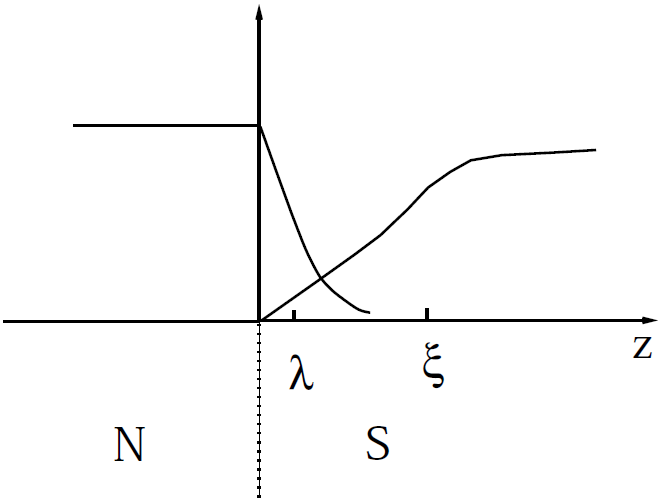
\includegraphics[width=0.45\textwidth]{immagini/GL_contributi_energetici.png}};
        % Rende disponibili le coordinate normalizzate (0..1, 0..1) sull'immagine
        \begin{scope}[x={(img.south east)}, y={(img.north west)}]
            % Esempi di disegni sopra:
            \node at (0.05,0.75) {$\dfrac{H}{H_c}$};
            \node[right] at (0.9,0.71) {$\dfrac{\psi(x)}{\psi_\infty}$};
        \end{scope}
    \end{tikzpicture}
\end{figure}
\hspace{-0.6cm}Stiamo integrando tra $-\infty$ e $+\infty$, quindi consideriamo sia la regione normale sia quella superconduttiva.\\
Nella regione normale sappiamo che il campo applicato è diverso da zero, quindi $\frac{H}{H_c}=1$, poiché siamo al campo critico.\\
Sappiamo però che il campo magnetico decade progressivamente all'interno del superconduttore, per cui all'interno di quest'ultimo assume un andamento come quello mostrato, con una scala caratteristica pari a $\lambda$.\\
L'altro contributo è quello del parametro d'ordine, che è nullo nella fase normale e diverso da zero nella fase superconduttiva. In particolare, esso tende al valore asintotico lontano dall'interfaccia e decade verso zero vicino all'interfaccia con una scala caratteristica $\xi$.\\
Vediamo ora il segno dell'energia.
\begin{figure}[H]
   \centering
   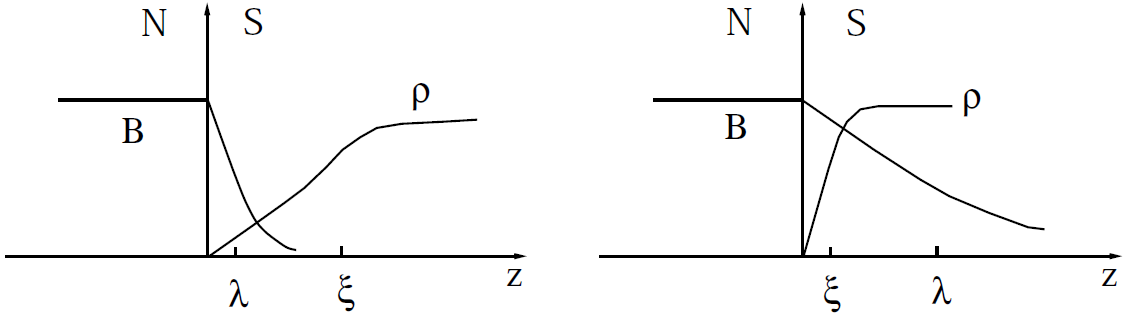
\includegraphics[width=0.8\textwidth]{immagini/energia_superficiale_superconduttore_tipo_I_e_II.png}
\end{figure}
\hspace{-0.6cm}Distinguiamo i due casi:
\begin{itemize}[leftmargin=0.5cm]
   \item Il caso $\kappa \ll 1$, cioè $\lambda \ll \xi$, è rappresentato a sinistra. In tale situazione si ottiene un'energia positiva. Ciò significa che non è conveniente avere molte superfici che separano le due fasi. Si ottiene quindi il comportamento tipico dei superconduttori di tipo I, nei quali compare essenzialmente un'unica superficie di separazione.
   \item Il caso opposto, $\kappa \gg 1$, cioè $\lambda \gg \xi$, è rappresentato a destra. In tale situazione il campo magnetico penetra profondamente nel materiale mentre il parametro d'ordine decade rapidamente vicino alla superficie. In questo caso abbiamo i superconduttori di tipo II. Qui è energeticamente conveniente avere molte superfici di separazione, e il campo penetra sotto forma di vortici.
\end{itemize}
Vediamo qualitativamente perché l'energia è positiva in un caso e negativa nell'altro:
\begin{figure}[H]
   \centering
   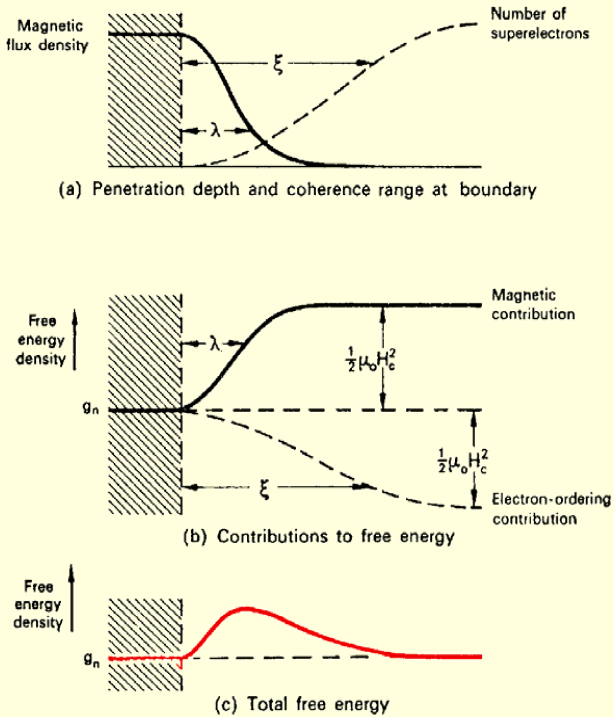
\includegraphics[width=0.45\textwidth]{immagini/energia_superficiale_positiva.png}
   \hspace{0.5cm}
   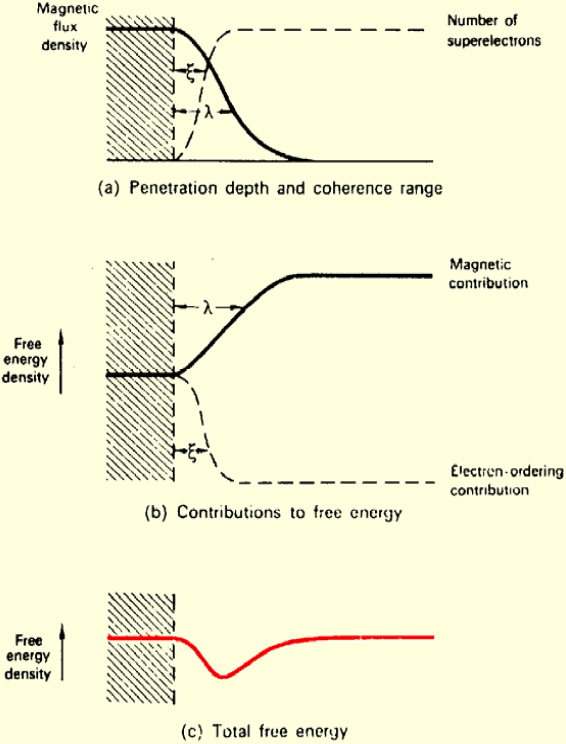
\includegraphics[width=0.45\textwidth]{immagini/energia_superficiale_negativa.png}
\end{figure}
\hspace{-0.6cm}Nel grafico sono mostrati i contributi all'energia libera superficiale, cioè i due termini che compaiono nell'integrale dell'\eqrefcustom{eq:contributo_superficiale_finale}.\\
Consideriamo dapprima il contributo magnetico, cioè $\qty(1-h/H_c)^2$. Avvicinandoci alla superficie, sappiamo che $h$ tende al campo applicato. Di conseguenza il termine $1-h/H_c$ parte da zero. Lontano dall'interfaccia, invece, $h\to 0$, quindi il termine tende a $1$.\\
Tra questi due limiti abbiamo un andamento continuo.\\
Consideriamo ora il contributo legato a $\psi$, $\abs{\psi/\psi_\infty}^4,$ che entra con segno negativo.\\
Vicino all'interfaccia siamo prossimi alla fase normale, quindi $\psi=0$ e il termine parte anch'esso da zero.\\
Per $x \to +\infty$, invece, $\psi \to \psi_\infty$, quindi il rapporto tende a $1$, ma compare con segno negativo nell'energia. Il contributo totale all'integrale è quindi negativo e ha un andamento come quello mostrato nel grafico.\\
Osserviamo che se $\lambda<\xi$, nel momento in cui sommiamo i due termini ci sarà una regione spaziale in cui il contributo totale resta positivo, e questo perché in tale regione il contributo associato al campo magnetico è maggiore del valore assoluto del contributo associato al parametro d'ordine, per cui prevale. In definitiva, in questo caso otteniamo un'energia superficiale che risulta positiva, tendendo a zero per $x\to 0 $ e per $x \to +\infty$.\\
Nel caso opposto, in cui $\xi \ll \lambda$, le scale spaziali si invertono, per cui il contributo negativo associato al parametro d'ordine prevale e la differenza tra i due termini diventa negativa. In questo caso avremo quindi un comportamento per l'energia superficiale tale per cui agli estremi tende ancora ad annullarsi, ma nel mezzo è sempre negativa.\\
Questo spiega perché, a seconda del rapporto tra profondità di penetrazione e lunghezza di coerenza, il costo energetico della superficie possa risultare positivo oppure negativo.\\
Per la maggior parte dei superconduttori elementari vale $\kappa<1$, quindi essi sono superconduttori di tipo I. Nei composti più complessi invece $\kappa$ è tipicamente molto maggiore di uno e il materiale appartiene alla classe dei superconduttori di tipo II.\\
Riassumendo:
\begin{itemize}[leftmargin=0.5cm]
   \item se $\xi>\lambda$, il sistema minimizza il numero di superfici tra fase normale e superconduttiva: questo corrisponde ai superconduttori di tipo I;
   \item se $\lambda>\xi$, il sistema preferisce avere molte regioni normali separate da fase superconduttiva: questo porta ai vortici dei superconduttori di tipo II.
\end{itemize}
Questa descrizione qualitativa emerge dalla teoria di Ginzburg--Landau.\\
La teoria quantitativa della transizione tra le due classi di superconduttori fu sviluppata da Abrikosov, che ricevette il premio Nobel nel 2003 insieme a Ginzburg e Leggett.\\
In quella teoria venne mostrato che il valore critico che separa i due comportamenti è
\begin{equation*}
   \kappa_c
   =
   \frac{1}{\sqrt{2}}
\end{equation*}
Inoltre fu possibile dimostrare che i vortici non si distribuiscono casualmente nel materiali, bensì esiste una configurazione di minima energia in cui i vortici formano un reticolo regolare. In particolare, il reticolo di vortici, detto reticolo di Abrikosov, è un reticolo triangolare, come mostrato nella figura seguente:
\begin{figure}[H]
   \centering
   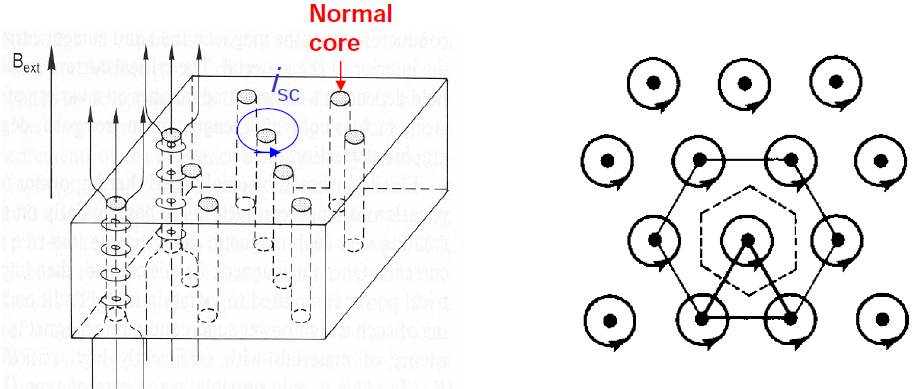
\includegraphics[width=0.7\textwidth]{immagini/Abrikosov_flux_Lattice.png}
\end{figure}
\hspace{-0.6cm}Questa è la tipica struttura della penetrazione del campo magnetico in un superconduttore di tipo II: abbiamo dei nuclei normali nei quali penetra il campo magnetico, i quali sono circondati da supercorrenti. Il comportamento è coerente con quanto già visto nella teoria di London, ma qui derivato in modo più accurato.\\
Fu inoltre possibile mostrare che i vortici non possono trasportare un flusso arbitrario. In altre parole, il flusso magnetico attraverso ciascun vortice può assumere soltanto valori pari a multipli interi del quanto di flusso $\Phi_0$, che è un fenomeno puramente quantistico.\\
La teoria permette anche di studiare l'interazione tra vortici, in particolare essi tendono a respingersi. Inoltre, se nel materiale sono presenti impurità, esse
tendono a rendere il materiale in loro prossimità in fase normale. Ciò significa che tipicamente i vortici tendono a localizzarsi in corrispondenza di queste impurità.\\
Osserviamo infine l'andamento della magnetizzazione in funzione del campo applicato nel caso dei superconduttori di tipo I e di tipo II:
\begin{figure}[H]
   \centering
   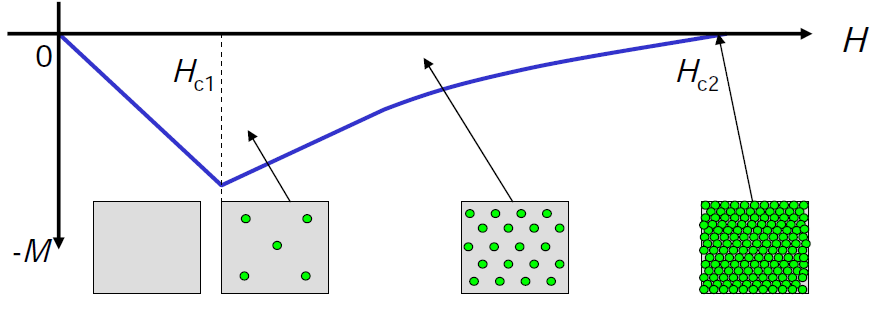
\includegraphics[width=0.8\textwidth]{immagini/andamento_magnetizzazione_superconduttore_tipo_I_e_II.png}
\end{figure}
\hspace{-0.6cm}Abbiamo già visto che in un superconduttore di tipo I si osserva il tipico comportamento diamagnetico fino al campo critico $H_c$.\\
In un superconduttore di tipo II, invece, compare una prima regione fino a un certo $H_{c,1}$ in cui il comportamento è identico a quello di un superconduttore di tipo I. Abbiamo poi una regione intermedia tra $H_{c,1}$ e $H_{c,2}$ in cui il campo penetra sotto forma di vortici, rappresentati nel grafico dai cerchi verdi. Notiamo come all'aumentare del campo magnetico, il numero di vortici aumenta e la loro densità diventa sempre più elevata, fino a riempire completamente il materiale in prossimità di $H_{c,2}$. Ciò non è altro che il materiale in fase normale per campi superiori a $H_{c,2}$.
\subsection{Stati intermedi nei superconduttori di tipo I}
Vediamo più nel dettaglio cosa accade nei superconduttori di tipo I.\\
Finora, quando abbiamo studiato ciò che accade in prossimità della superficie che separa la fase normale da quella superconduttiva (oppure il vuoto dalla fase superconduttiva) abbiamo considerato una geometria molto semplice. In particolare, abbiamo considerato la situazione in cui si applica un campo magnetico parallelo alla superficie di separazione tra il semispazio vuoto e il semispazio superconduttivo.\\
In realtà, le cose sono un po' più complicate se la superficie del materiale non ha una geometria così semplice, ma possiede invece una forma arbitraria. In questo caso la situazione non è così immediata, perché può verificarsi una penetrazione del campo magnetico anche nei superconduttori di tipo I.\\
In altre parole, in geometrie più complesse rispetto a quella discussa finora, possiamo avere la coesistenza di fasi normali e superconduttive, pur restando in una situazione completamente diversa dalla fase a vortici dei superconduttori di tipo II.\\
L'esempio più semplice è il caso di un superconduttore di forma sferica immerso in una regione in cui è presente un campo magnetico applicato $H_a$:
\begin{figure}[H]
   \centering
   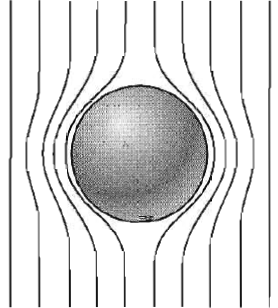
\includegraphics[width=0.25\textwidth]{immagini/sfera_superconduttiva.png}
\end{figure}
\hspace{-0.6cm}Lontano dalla sfera, il campo è uniforme e orientato lungo una certa direzione.\\
Avvicinandosi però al materiale superconduttivo, a causa dell'effetto Meissner il campo magnetico viene espulso. Questo implica che le linee di campo vicino alla superficie si deformano, assumendo una configurazione  tale che in prossimità del piano equatoriale le linee di campo diventano sempre più fitte.\\
Questo significa che il campo magnetico vicino alla superficie, in particolare nella regione equatoriale, aumenta di intensità, perché una maggiore densità di linee di campo corrisponde a un campo magnetico più intenso.\\
Risolvendo le equazioni di Maxwell si può mostrare che, vicino al piano equatoriale, il campo tangenziale alla superficie assume il valore
\begin{equation*}
   H_t=\frac{3}{2}H_a
\end{equation*}
Questo significa che, anche se applichiamo un campo magnetico $H_a$ minore del campo critico $H_c$, la situazione reale non è così semplice come ci si potrebbe aspettare intuitivamente.\\
Infatti, ingenuamente potremmo pensare che, finché $H_a < H_c$ il campo magnetico venga completamente espulso dal materiale. Tuttavia, il punto fondamentale è che il campo effettivamente percepito dalla superficie del materiale — in particolare vicino al piano equatoriale — non è $H_a$, bensì $\frac{3}{2}H_a$. Di conseguenza, il materiale può trovarsi localmente in condizioni tali da permettere la penetrazione del campo magnetico anche se il campo applicato lontano dal campione è ancora minore di $H_c$.\\
In particolare, se il campo applicato soddisfa
\begin{equation*}
   \frac{2}{3}H_c < H_a < H_c
\end{equation*}
si avrà la coesistenza di fase normale e fase superconduttiva all'interno del materiale.\\
Questo esempio riguarda il caso sferico, ma fenomeni analoghi si verificano anche per materiali con forme differenti.\\
Si introduce allora il cosiddetto fattore di demagnetizzazione $\eta$, definito in modo tale che, quando il campo applicato soddisfa
\begin{equation*}
   1-\eta < \frac{H_a}{H_c} < 1
\end{equation*}
si ha la coesistenza delle fasi normale e superconduttiva, cioè una penetrazione parziale del campo magnetico nel materiale.\\
In altre parole, $\eta$ quantifica quanto il campo magnetico applicato possa penetrare nel materiale anche se il valore del campo esterno è inferiore a $H_c$, che sarebbe invece il valore critico nel caso semplice di un campo parallelo alla superficie.\\
A questo punto ci chiediamo come penetri nel materiale il campo magnetico in queste condizioni. Supponiamo di avere un materiale cilindrico:
\begin{figure}[H]
   \centering
   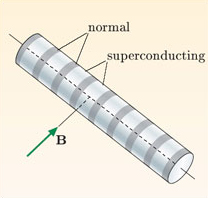
\includegraphics[width=0.4\textwidth]{immagini/cilindro_superconduttivo.png}
\end{figure}
\hspace{-0.6cm}Si può mostrare che se il campo magnetico è parallelo all'asse del cilindro, il comportamento è analogo a quello già visto nel caso di una lastra piana: il campo penetra soltanto entro una profondità dell'ordine di $\lambda$; se invece il campo magnetico è perpendicolare all'asse del cilindro, la situazione cambia completamente. In quest'ultimo caso si ha una deformazione delle linee di campo analoga a quella discussa per la sfera.\\
Di conseguenza, può verificarsi una penetrazione parziale del campo magnetico anche per valori di $B$ minori di $H_c$.\\
Si può mostrare che il campo penetra sotto forma di regioni laminate alternate, quindi avremo un'alternanza di lamelle normali e superconduttive. La penetrazione del campo avviene quindi in maniera laminare e non tramite vortici.\\
Come si osserva sperimentalmente questo fenomeno?\\
Se il sistema è immerso in un campo magnetico orientato perpendicolarmente all'asse del cilindro, il materiale diventa superconduttivo e presenta resistenza nulla per correnti che scorrono perpendicolarmente all'asse del cilindro.\\
Tuttavia, poiché il campo penetra tramite strati alternati normali e superconduttivi, una corrente che scorra lungo l'asse attraverserà un alternarsi di regioni a resistenza nulla e poi resistive. Di conseguenza il trasporto lungo questa direzione risulterà dissipativo.\\
Se invece consideriamo una corrente che fluisce perpendicolarmente all'asse del cilindro, il contributo delle regioni superconduttive prevale e il sistema si comporterà prevalentemente come un superconduttore, senza manifestare una resistenza apprezzabile.\\
Un comportamento analogo si osserva anche in una geometria a lastra piana:
\begin{figure}[H]
   \centering
   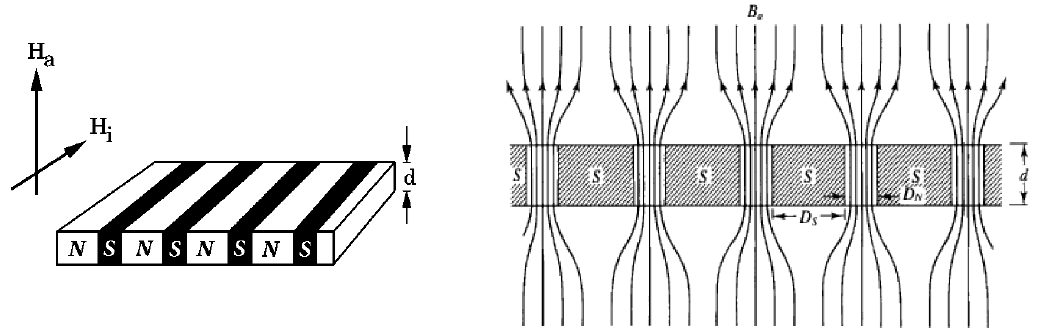
\includegraphics[width=0.9\textwidth]{immagini/lastra_superconduttiva.png}
\end{figure}
\hspace{-0.6cm}Se il campo magnetico è applicato perpendicolarmente alla lastra, la soluzione delle equazioni di Ginzburg--Landau o di London mostra ancora una volta che il campo penetra tramite un'alternanza di regioni normali e superconduttive.\\
Questo comportamento potrebbe ricordare quello dei vortici nei superconduttori di tipo II, ma in realtà si tratta di un fenomeno completamente diverso. La differenza fondamentale è che in questo caso le regioni normali in cui il campo magnetico è diverso da zero sono macroscopiche. Di conseguenza, il flusso magnetico che attraversa tali regioni non è quantizzato, cioè non è un multiplo intero del quanto di flusso $\Phi_0$. Inoltre, se osserviamo la lastra dall'alto, vediamo chiaramente l'alternanza di strisce normali e superconduttive.\\
Questo tipo di penetrazione prende il nome di penetrazione laminare.\\
Il messaggio fondamentale è quindi il seguente:
\begin{itemize}[leftmargin=0.5cm]
   \item anche nei superconduttori di tipo I il campo magnetico può penetrare nel materiale;
   \item ciò può dare origine alla coesistenza di regioni normali e superconduttive;
   \item la penetrazione avviene però tramite domini normali macroscopici e non tramite vortici quantizzati;
   \item il fenomeno dipende fortemente dalla geometria del campione e dalla direzione del campo magnetico rispetto alla superficie.
\end{itemize}
\subsection{Effetto di prossimità}
L'effetto di prossimità è un fenomeno che si verifica in generale tra due metalli quando almeno uno dei due è superconduttore. L'altro può trovarsi nella fase normale oppure entrambi possono essere materiali superconduttivi caratterizzati però da differenti temperature critiche, $T_{c,A}$ e $T_{c,B}$, con $T_{c,A}>T_{c,B}$.\\
Supponiamo di avere l'interfaccia tra questi due superconduttori. Se eseguiamo un esperimento abbassando progressivamente la temperatura, il materiale con temperatura critica maggiore diventerà superconduttivo per primo, mentre l'altro si troverà ancora nella fase normale.\\
Quando esiste una superficie che separa i due materiali, il materiale con temperatura critica più alta può "indurre" la superconduttività nel materiale vicino. Questo fenomeno prende il nome di effetto di prossimità.\\
Ciò significa che gli elettroni del materiale posto a contatto con il superconduttore a temperatura critica più alta possono anch'essi entrare nella fase superconduttiva. Questo accade anche se la temperatura del materiale $B$ è ancora maggiore della sua temperatura critica intrinseca.\\
Dal punto di vista tecnologico questo effetto è particolarmente importante. Immaginiamo infatti di avere un materiale con temperatura critica sufficientemente alta e, nelle sue vicinanze, uno strato molto sottile di un altro materiale avente una temperatura critica molto più piccola di $T_{c,A}$.\\
Per portare quest'ultimo nella fase superconduttiva dovremmo normalmente abbassare notevolmente la temperatura. Tuttavia, se lo strato viene posto sufficientemente vicino al materiale con temperatura critica più alta, esso può diventare superconduttivo proprio grazie all'effetto di prossimità.\\
In altre parole, il materiale può entrare nella fase superconduttiva pur trovandosi a una temperatura maggiore della sua temperatura critica intrinseca.\\
Questo è il fenomeno che si osserva, ad esempio, in geometrie nelle quali abbiamo un superconduttore da un lato e un altro superconduttore dall'altro lato — supponiamo identici, quindi entrambi caratterizzati dalla stessa temperatura critica $T_{c,B}$ — separati da uno strato estremamente sottile di un altro materiale.\\
Nel limite più estremo questo strato può avere lo spessore di un singolo atomo. È proprio ciò che accade tipicamente nel caso del grafene, che sarà oggetto dell'ultima parte del corso.\\
Il grafene è essenzialmente un materiale bidimensionale: il suo spessore nella direzione perpendicolare al piano è dell'ordine di un singolo strato atomico.\\
Essendo costituito da carbonio, il grafene è normalmente un metallo con una particolare struttura a bande. Il suo spettro elettronico differisce da quello di un metallo convenzionale.\\
Quando però inseriamo questo sottilissimo strato di grafene tra due superconduttori, si manifesta proprio l'effetto di prossimità.\\
Ciò significa che può fluire una supercorrente tra i due superconduttori attraversando lo strato bidimensionale di grafene.\\
In questo caso otteniamo una giunzione superconduttiva nella quale compare il cosiddetto effetto Josephson attraverso uno strato di grafene: una graphene Josephson junction.\\
Nel corso parleremo più avanti delle giunzioni Josephson. Nel nostro caso esse saranno costituite da due superconduttori separati da uno strato isolante oppure da uno strato di materiale conduttivo. Vedremo che anche in quel caso può fluire una supercorrente. In generale il meccanismo sarà diverso dall'effetto di prossimità discusso qui.
\subsection{Quantizzazione del flusso}
Vediamo quali sono le implicazioni della teoria di Ginzburg--Landau per quanto riguarda la connessione tra campo magnetico e differenti geometrie del superconduttore. Questo ci porterà alla quantizzazione del flusso. Inoltre, analizzeremo anche la natura della transizione che avviene nel passaggio dalla fase normale alla fase superconduttiva e, in particolare, quale simmetria venga rotta durante questa transizione.\\
L'idea è capire che cosa accade al campo magnetico quando abbiamo un materiale superconduttivo e partiamo dalla descrizione in termini del parametro d'ordine complesso. Vedremo infatti che tutti questi fenomeni sono profondamente legati proprio alla natura complessa del parametro d'ordine.\\
Il parametro d'ordine $\psi(\vb{r})$ deve essere una funzione ad un sol valore. Questo significa che l'integrale lungo una linea chiusa del gradiente della fase $\phi$ deve essere pari a un multiplo intero di $2\pi$:
\begin{equation}
    \oint \grad{\phi} \vdot \dd{\vb{s}}
    =
    2\pi n
    \label{eq:integrale_phi_curva_chiusa}
\end{equation}
Vediamo quali implicazioni abbia questa proprietà sulla densità di supercorrente, che abbiamo già visto poter essere espressa tramite l'\eqrefcustom{eq:densita_di_supercorrente}, con $|\psi|^2$ che identifica la densità di elettroni superconduttivi $n_s$.\\
Da questa identità possiamo anche scrivere il momento quantistico nella forma
\begin{equation*}
    m^*\vb{v}_s
    =
    \hbar \grad{\phi}
    -
    \frac{e^*}{c}\vb{A}.
\end{equation*}
Poiché deve valere la \eqref{eq:integrale_phi_curva_chiusa}, deve risultare
\begin{equation}
   \oint \qty[ m^* \vb{v}_s + \frac{e^*}{c}\vb{A} ] \vdot \dd{\vb{s}}
   =\hbar 2\pi n
   \label{eq:integrale_momento_curva_chiusa}
\end{equation}
Cioè, se integriamo lungo una linea chiusa questa combinazione di termini — che corrisponde a $\grad{\phi}$ — dobbiamo ottenere $\hbar 2\pi n$.\\
Osserviamo ora che l'integrale del potenziale vettore è in realtà uguale al flusso del campo magnetico, purché la linea e la superficie siano legate dalla condizione che la prima sia il bordo della seconda:
\begin{equation}
   \oint \vb{A}\vdot\dd{\vb{s}}
   =
   \int_{\Sigma}\vb{h}\vdot\dd{\vb*{\Sigma}}
   \label{eq:integrale_A_flusso_B}
\end{equation}
dove abbiamo usato $\vb{h}$ invece di $\vb{B}$ perché intendiamo il campo magnetico locale.\\
Possiamo quindi riscrivere la relazione precedente esprimendo l'integrale di linea di $\vb{A}$ in termini del flusso del campo magnetico. Moltiplicando per $c/e^*$ otteniamo
\begin{equation*}
    \int_{\Sigma}
    \vb{h}\vdot\dd{\vb*{\Sigma}}
    +
    \frac{c}{e^*}
    \oint
    m^*\vb{v}_s\vdot\dd{\vb{s}}
    =
    2\pi n\frac{c\hbar}{e^*}
    \equiv
    n\Phi_0
\end{equation*}
Il risultato che troviamo è una quantità avente le dimensioni di un flusso magnetico. Questo ci dice che la combinazione tra il flusso del campo magnetico in una geometria generica e il contributo associato al momento dei portatori deve essere uguale a un multiplo intero di una quantità che ha le dimensioni di flusso magnetico.\\
Questa condizione prende il nome di \emph{condizione di quantizzazione del flussoide} (\emph{fluxoid quantization condition}), dove il quanto di flussoide è
\begin{equation*}
   \Phi_0
   =
   2\pi\hbar\frac{c}{2e}
   =
   2.07\times10^{-7}\,\text{Gauss cm}^2,
\end{equation*}
avendo posto la carica efficace dei portatori pari a $2e$ (risultato che emerge rigorosamente dalla teoria BCS). Questa quantità è chiamata \emph{quanto di flusso}.\\
Vediamo ora quali siano le implicazioni di questa condizione nei diversi casi possibili:
\begin{itemize}[leftmargin=0.5cm]
   \item all'interno del bulk di un superconduttore;
   \item nel caso in cui esistano regioni normali all'interno del superconduttore;
   \item nel caso di un superconduttore con geometria ad anello.
\end{itemize}
Vedremo che, a seconda della situazione, questa relazione conduce a conseguenze differenti.\\[0.2cm]
\textbf{Primo caso: bulk completamente superconduttivo}\\
Supponiamo di avere un materiale bulk interamente nella fase superconduttiva, senza alcuna regione normale interna, e consideriamo un contorno chiuso all'interno del materiale.
\begin{figure}[H]
   \centering
   \begin{tikzpicture}[scale=1.5]
      % Cerchio interno
      \begin{scope}[canvas is xz plane at y=0]
         \draw[thick, red, opacity=0.75] (1.6,0.5) circle (0.8);
      \end{scope}
      % Faccia frontale semi-trasparente, sopra il cerchio
      \draw[ fill=gray!40, fill opacity=0.65, draw=black] (0,0,0) -- (0,-1,0) -- (2,-1,0) -- (2,0,0) -- cycle;
      % Faccia superiore e laterale, dietro
      \draw[fill=gray!70, fill opacity=0.65, draw=black] (0,0,0) -- (0,0,-2) -- (2,0,-2) -- (2,0,0) -- cycle;
      \draw[fill=gray!55, fill opacity=0.65, draw=black] (2,0,0) -- (2,0,-2) -- (2,-1,-2) -- (2,-1,0) -- cycle;
   \end{tikzpicture}
\end{figure}
\hspace{-0.6cm}Poiché siamo nel bulk del superconduttore, per effetto Meissner sappiamo che il campo magnetico deve essere nullo. Ma se il campo magnetico è nullo nella parte interna del materiale, allora deve essere nulla anche la supercorrente, dato che essa scorre soltanto in prossimità della superficie.\\
In queste condizioni abbiamo quindi che $\vb{h}=0$ e $\vb{J}_s=0$. Da ciò segue che l'intero $n$ deve essere uguale a zero. Tornando allora all'\eqrefcustom{eq:integrale_phi_curva_chiusa}, otteniamo
\begin{equation*}
   \oint \grad{\phi} \vdot \dd{\vb{s}}=0
\end{equation*}
e ciò implica che la fase non può dipendere dalla posizione all'interno del bulk del superconduttore: la fase $\phi$ deve quindi essere uniforme.\\
Questa è un'osservazione molto importante, perché implica che nel bulk del superconduttore il parametro d'ordine può avere un modulo dipendente dalla posizione, ma il fattore di fase deve essere costante:
\begin{equation*}
      \psi(\vb{r})
      =
      |\psi(\vb{r})|e^{i\phi}
\end{equation*}
Vedremo che questo risultato è legato anche al tipo di simmetria che viene rotta durante la transizione superconduttiva.\\[0.2cm]
\textbf{Secondo caso: presenza di regioni normali}\\
Consideriamo ora il caso in cui siamo ancora all'interno del bulk di un materiale superconduttivo, ma siano presenti alcune regioni normali.\\
Supponiamo, ad esempio, di avere un vortice, cioè una regione nella quale il campo magnetico penetra all'interno del materiale.
\begin{figure}[H]
   \centering
   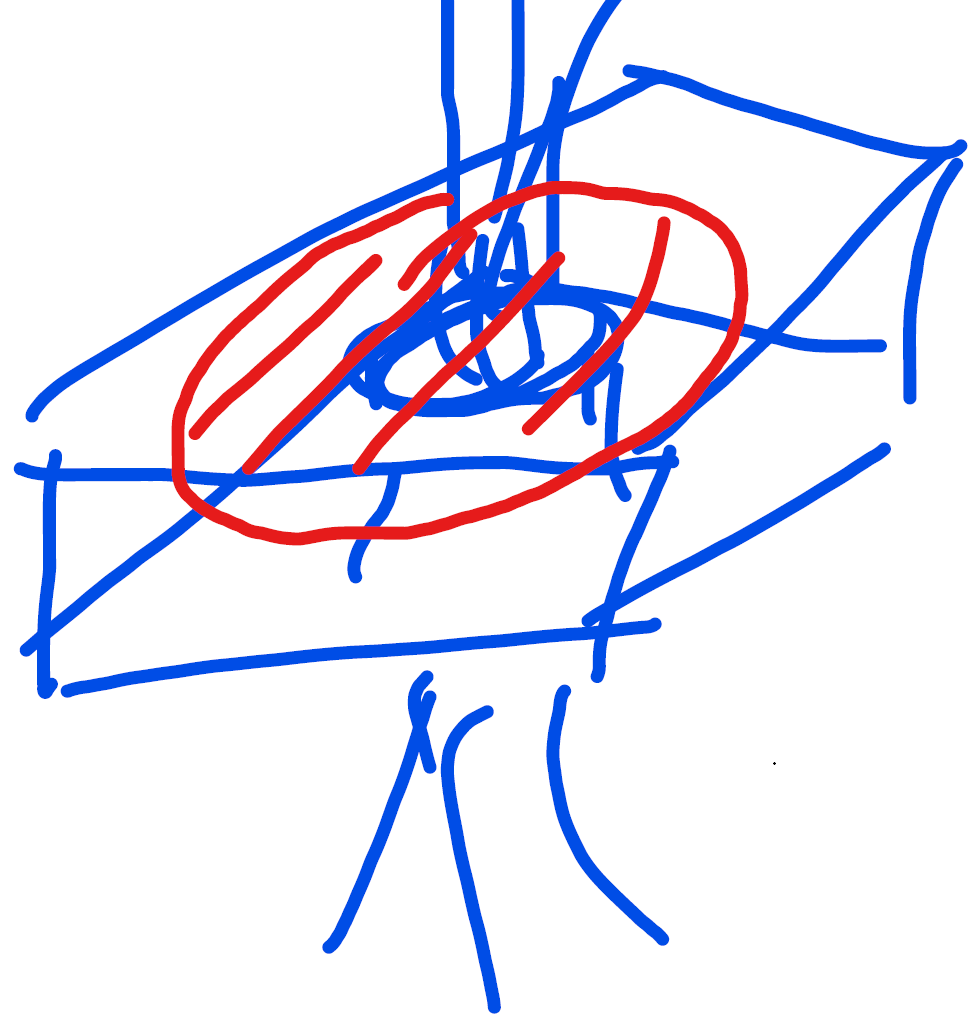
\includegraphics[width=0.3\textwidth]{immagini/fluxoid_quantization_vortice.png}
\end{figure}
\hspace{-0.6cm}Se scegliamo un contorno che circonda questa regione normale, ci troviamo ancora nella situazione in cui la densità superconduttiva è nulla lontano dalla superficie, quindi $\vb{J}_s=0$, ma il campo magnetico attraversa la superficie delimitata dal contorno.\\
In questo caso, l'\eqrefcustom{eq:integrale_momento_curva_chiusa} implica allora che il flusso del campo magnetico attraverso tale superficie deve essere uguale a un multiplo intero del quanto di flusso:
\begin{equation*}
   \int_{\Sigma} \vb{h}\vdot\dd{\vb*{\Sigma}}
   =2\pi n\frac{c\hbar}{e^*}
   \equiv n\Phi_0
\end{equation*}
Questa non è altro che la condizione che avevamo già menzionato parlando dei superconduttori di tipo II. Essa ci dice che il flusso magnetico che penetra nel superconduttore non può assumere valori arbitrari, ma deve essere quantizzato.\\
Per esempio, nel caso dei superconduttori di tipo II, dove il campo magnetico penetra nel materiale, i flussi $\Phi_1, \Phi_2, \ldots$ associati ai campi magnetici $h_1, h_2, \ldots$ non possono essere arbitrari. Essi devono necessariamente essere pari a $n_1\Phi_0, n_2\Phi_0, \dots$, cioè a multipli interi del quanto di flusso.\\[0.2cm]
\textbf{Terzo caso: anello superconduttivo}\\
Consideriamo infine un anello superconduttivo.
\begin{figure}[H]
   \centering
   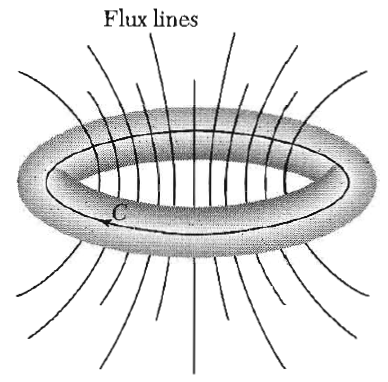
\includegraphics[width=0.4\textwidth]{immagini/fluxoid_quantization_anello.png}
\end{figure}
\hspace{-0.6cm}Supponiamo di prendere un contorno all'interno dell'anello come mostrato. In questo caso, nella parte interna del materiale superconduttivo abbiamo ancora $\vb{h}=0$ e $\vb{J}_s=0$, ma la superficie delimitata dal contorno racchiude una regione vuota nella quale il campo magnetico può penetrare. Di conseguenza, esiste un flusso magnetico non nullo attraverso tale superficie.\\
Anche in questo caso, la condizione di quantizzazione appena ottenuta implica che il flusso debba essere un multiplo intero del quanto di flusso.\\
Questo significa che, se raffreddiamo un anello superconduttivo in presenza di un campo magnetico, quando il sistema attraversa la transizione superconduttiva e successivamente il campo magnetico esterno viene spento, all'interno dell'anello rimane intrappolato un flusso magnetico quantizzato.\\
Ciò avviene perché continua a circolare una supercorrente lungo l'anello, la quale genera un campo magnetico che resta confinato all'interno della geometria ad anello.\\
La differenza rispetto al caso precedente è che qui stiamo considerando una struttura costruita artificialmente, mentre nel caso del bulk con vortici il sistema sviluppa spontaneamente regioni normali all'interno del materiale.\\
Il risultato fondamentale è comunque lo stesso, in quanto il flusso magnetico intrappolato nell'anello non è arbitrario, ma deve essere necessariamente uguale a un multiplo intero di $\Phi_0$, e ciò qualunque sia la grandezza dell'anello.\\
Per comprendere meglio il significato di questo risultato, proviamo ora a derivarlo dal punto di vista energetico.\\
Se il sistema si comporta in questo modo, significa che deve essere energeticamente conveniente trovarsi in una configurazione in cui il flusso magnetico è quantizzato.\\
Dobbiamo quindi partire dall'espressione dell'energia libera in una situazione di questo tipo e vedere quale forma assume.\\
Per farlo, descriviamo il sistema mediante coordinate polari cilindriche, $\vb{r} = (r,\varphi,z)$, con l'asse $z$ perpendicolare al piano dell'anello.\\ Supponiamo innanzitutto che le variazioni di $\psi(\vb{r})$ attraverso la sezione trasversale dell'anello siano trascurabili; possiamo quindi ignorare qualsiasi dipendenza da $r$ e $z$, dunque $\psi(\vb{r})=\psi(\varphi)$.\\ 
Inoltre, affinché il parametro d'ordine sia una funzione ad un solo valore, esso deve essere periodico nell'angolo $\varphi$:
\begin{equation}
   \psi(\varphi+2\pi)=\psi(\varphi)
   \label{eq:condizione_singolo_valore_psi}
\end{equation}
Ciò implica che la dipendenza funzionale di $\psi(\varphi)$ debba essere di tipo esponenziale:
\begin{equation*}
   \psi(\varphi)=\psi_0 e^{in\varphi}
\end{equation*}
dove $n$ rappresenta un numero di avvolgimenti.\\
Per rendere la trattazione il più semplice possibile, assumiamo inoltre che il campo magnetico sia uniforme all'interno dell'anello.\\
In queste condizioni esiste una relazione semplice tra l'integrale di linea del potenziale vettore e il flusso del campo magnetico. Possiamo infatti assumere che $\vb{A}$ sia costante lungo l'anello e quindi dall'\eqrefcustom{eq:integrale_A_flusso_B} segue
\begin{equation*}
   \Phi(\vb{B}) = A\,2\pi R
\end{equation*}
da cui
\begin{equation}
   \vb{A} = \frac{\Phi(\vb{B})}{2\pi R}\vu{u}_{\varphi}
   \label{eq:vector_potential_ring}
\end{equation}
Con queste ipotesi possiamo inserire le proprietà appena trovate nell'energia libera di Ginzburg--Landau.\\
Abbiamo visto che l'energia libera della fase superconduttiva può essere scritta come somma dell'energia libera della fase normale e del contributo di Ginzburg--Landau:
\begin{equation*}
   \begin{split}
      F_s
      &=
      F_n
      +
      \int \dd[3]{\vb{r}}
      \qty{
      \frac{\hbar^2}{2m^*}
      \qty|
      \qty(
         \grad
         +
         i\frac{2e}{c\hbar}\vb{A}
      )\psi
      |^2
      +
      a|\psi|^2
      +
      \frac{b}{4}|\psi|^4
      }
      +
      E_B
      \\
      &=
      F_s^0
      +
      \int \dd[3]{\vb{r}}
      \qty{
      \frac{\hbar^2}{2m^*}
      \qty|
      \qty(
         \grad
         +
         i\frac{2e}{c\hbar}\vb{A}
      )\psi
      |^2
      }
      +
      E_B
   \end{split}
\end{equation*}
dove
\begin{equation*}
   F_s^0
   =
   F_n
   +
   \int \dd[3]{\vb{r}}
   \qty{
   a|\psi|^2
   +
   \frac{b}{4}|\psi|^4
   }
\end{equation*}
è l'energia libera dello stato fondamentale dell'anello in assenza di correnti e di flussi magnetici, mentre $E_B$ rappresenta il contributo energetico del campo magnetico.\\
Usando ora l'\eqrefcustom{eq:condizione_singolo_valore_psi} e l'\eqrefcustom{eq:vector_potential_ring}, otteniamo\mn{Ricordiamo che dobbiamo usare il gradiente in coordinate cilindriche, ma avendo dipendenza soltanto da $\varphi$, esso diventa semplicemente
\begin{equation*}
   \grad=\frac{1}{r}\partial_\varphi \vu{u}_\varphi
\end{equation*}}
\begin{equation*}
   \qty(
      \grad
      +
      i\frac{2e}{c\hbar}\vb{A}
   )\psi
   =
   \qty(
      -i\frac{n}{R}
      +
      i\frac{2e}{c\hbar}
      \frac{\Phi(\vb{B})}{2\pi R}
   )
   \psi\vu{u}_\varphi.
\end{equation*}
Segue quindi che
\begin{equation*}
   \frac{\hbar^2}{2m^*}
   \qty|
   \qty(
      \grad
      +
      i\frac{2e}{c\hbar}\vb{A}
   )\psi
   |^2
   =
   \frac{\hbar^2}{2m^*R^2}
   \qty[
      n-\frac{\Phi(\vb{B})}{\Phi_0}
   ]^2
   |\psi|^2,
\end{equation*}
dove $\Phi_0=\frac{hc}{2e}$.\\
Integrando sul volume dell'anello otteniamo
\begin{equation*}
   \int \dd[3]{\vb{r}}
   \qty{
   \frac{\hbar^2}{2m^*}
   \qty|
   \qty(
      \grad
      +
      i\frac{2e}{c\hbar}\vb{A}
   )\psi
   |^2
   }
   =
   V
   \frac{\hbar^2}{2m^*R^2}
   \qty[
      n-\frac{\Phi(\vb{B})}{\Phi_0}
   ]^2
   |\psi|^2
\end{equation*}
Ricordiamo ora che conosciamo anche l'espressione del contributo energetico del campo magnetico. Infatti, poiché l'energia del campo magnetico è data dall'integrale sul volume interno all'anello, abbiamo
\begin{equation*}
   E_B
   =
   \int\displaylimits_{
      \begin{subarray}{c}
         \text{parte}\\
         \text{interna}
      \end{subarray}
   }
   \dd[3]{\vb{r}}
   \frac{B^2}{8\pi}
\end{equation*}
Questa espressione può essere riscritta in termini dell'autoinduttanza dell'anello:
\begin{equation*}
   E_B=\frac{1}{2}LI^2
\end{equation*}
Scrivendo il flusso magnetico nella forma $\Phi(\vb{B})=LI$, si ottiene infine
\begin{equation*}
   E_B = \frac{1}{2}\frac{\Phi^2}{L}
\end{equation*}
In conclusione, otteniamo
\begin{equation*}
   F_s
   =
   F_s^{\rm bulk}
   +
   \text{const.}
   \times
   \qty[
      n-\frac{\Phi(\vb{B})}{\Phi_0}
   ]^2
   |\psi|^2
   +
   \frac{1}{2}\frac{\Phi^2}{L}
\end{equation*}
Possiamo ora rappresentare queste energie in funzione del flusso $\Phi$:
\begin{figure}[H]
   \centering
   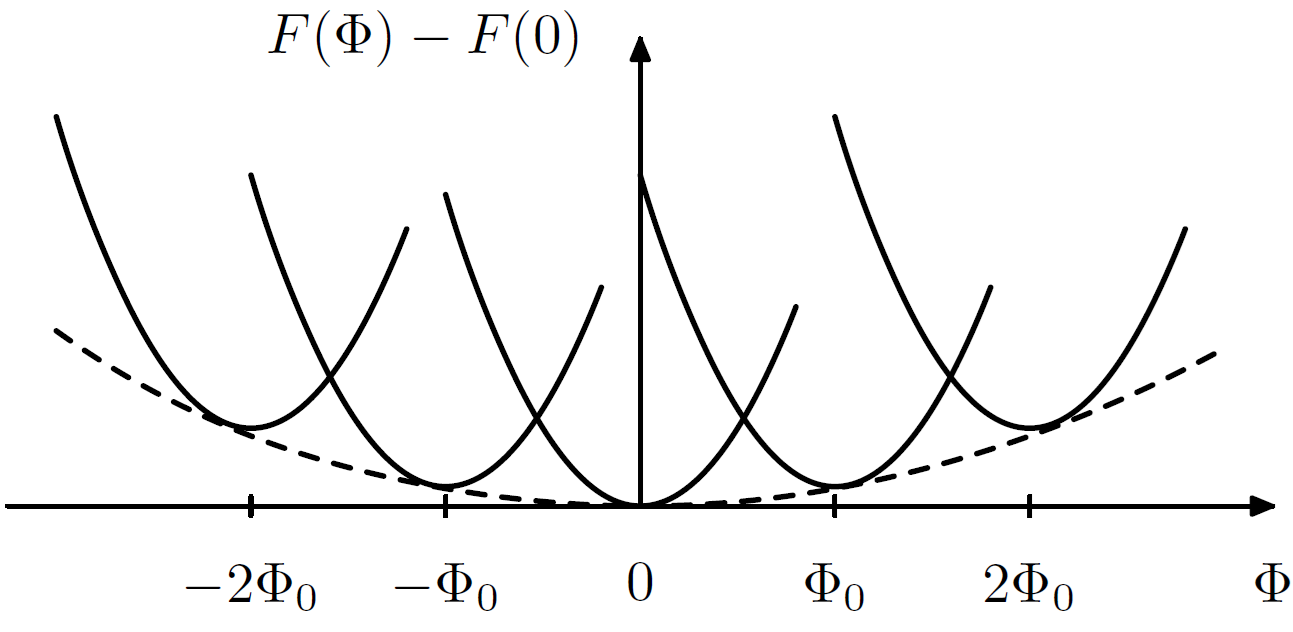
\includegraphics[width=0.6\textwidth]{immagini/energy_flux_quantization.png}
\end{figure}
\hspace{-0.6cm}Abbiamo la somma di due contributi: un termine puramente parabolico (rappresentato dalla linea tratteggiata) e una famiglia di parabole dipendenti da $n$. I minimi di tali parabole si trovano in corrispondenza della condizione
\begin{equation*}
   \frac{\Phi(\vb{B})}{\Phi_0}=n
\end{equation*}
quindi, per esempio, per $n=0$ la parabola è centrata in $\Phi=0$; per $n=1$ la parabola è centrata in $\Phi=\Phi_0$ e così via.\\
In definitiva, l'energia totale, data dalla somma di questi contributi, presenta una serie di minimi metastabili e lo stato finale del sistema (uno di questi minimi) dipenderà dalla storia del campo magnetico applicato. Per esempio, se il flusso iniziale è vicino a $\Phi_0$, il sistema rilasserà verso il minimo più vicino, cioè verso il minimo per $n=1$. In generale, la configurazione stabile sarà quella corrispondente al minimo energetico più vicino alla condizione iniziale.\\
Possiamo ora aggiungere un ulteriore ingrediente alla descrizione, che sarà rilevante nel seguito. Supponiamo di interpretare questa struttura come il paesaggio di energia potenziale visto da un sistema quantistico. In questo caso, abbiamo una serie di pozzi di potenziale separati da barriere.
\begin{figure}[H]
   \centering
   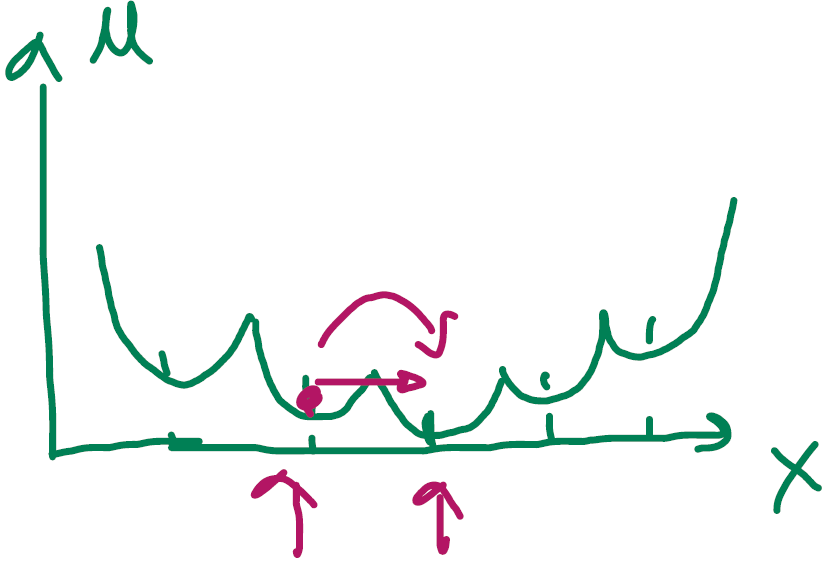
\includegraphics[width=0.5\textwidth]{immagini/energy_landscape_quantization.png}
\end{figure}
\hspace{-0.6cm}In meccanica quantistica, una particella descritta da una funzione d'onda può tunnelare da un minimo all'altro. Applicando questa idea al problema dell'anello superconduttivo, possiamo immaginare processi nei quali il sistema passa da un minimo metastabile al successivo tramite tunneling quantistico.\\
In termini della fase, ciò corrisponde al passaggio da $\phi$ a $\phi + 2\pi$, mentre dal punto di vista del numero di winding, ciò significa passare da $n$ a $n\pm1$.\\
Questi processi prendono il nome di \emph{phase slips}. Essi corrispondono quindi a cambiamenti discreti del numero di winding associati a processi di tunneling quantistico.\\
Poiché la supercorrente dipende da $n$, un cambiamento di $n$ implica anche una variazione della supercorrente che circola nell'anello.\\
Questi processi possono avvenire per tunneling quantistico a temperatura nulla oppure per attivazione termica a temperatura finita. A temperatura finita infatti gli stati eccitati sono popolati e possono attraversare più facilmente la barriera di potenziale oppure superarla termicamente.\\
In questo modo si hanno processi di decadimento della supercorrente.\\
L'aspetto più notevole è che, se facciamo un passo indietro e ricordiamo che il sistema è costituito da un enorme numero di elettroni, ci rendiamo conto che questi processi rappresentano tunneling quantistico macroscopico. Questo è alla base di fenomeni come il macroscopic quantum tunneling e la macroscopic quantum coherence, che verranno descritti in modo rigoroso dalla teoria BCS, nella quale introdurremo una vera funzione d'onda del condensato. Tuttavia, già nella teoria di Ginzburg--Landau emerge naturalmente una descrizione di questo tipo se interpretiamo il parametro d'ordine come una funzione d'onda macroscopica dell'intero sistema.\\
Naturalmente, manca ancora una giustificazione microscopica rigorosa, che verrà introdotta successivamente.\\
È comunque importante osservare quanto fosse profonda l'intuizione alla base della teoria di Ginzburg--Landau, in quanto essa riuscì a prevedere fenomeni estremamente non banali pur senza una teoria microscopica completa, utilizzando soltanto una descrizione fenomenologica basata sull'energia libera.\\
Consideriamo infine il seguente quadro qualitativo:
\begin{figure}[H]
   \centering
   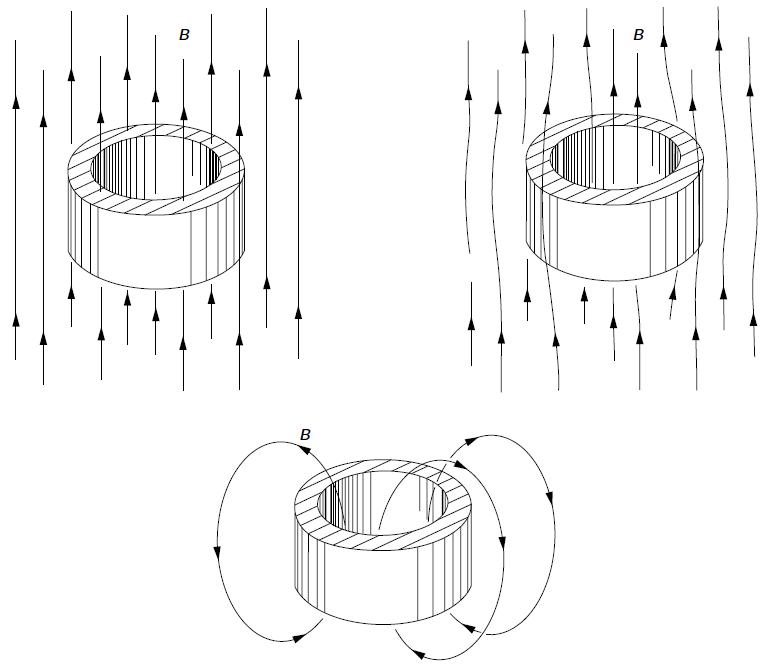
\includegraphics[width=0.7\textwidth]{immagini/flux_quantization_experiment.png}
\end{figure}
\hspace{-0.6cm}Partiamo da un anello superconduttivo nella fase normale immerso in un campo magnetico. Quando abbassiamo la temperatura al di sotto di $T_c$, il sistema entra nella fase superconduttiva e il campo magnetico viene espulso. Una parte del flusso resta intrappolata all'interno dell'anello e rimane confinato anche quando il campo magnetico esterno viene spento.\\
Il punto fondamentale è che il flusso intrappolato non può assumere valori arbitrari, ma solo multipli del quanto di flusso: $\Phi=n\Phi_0$.\\
Questo effetto fu misurato sperimentalmente nel 1961 da due gruppi differenti e rappresenta uno dei primi esempi di fenomeno quantistico macroscopico osservato sperimentalmente.
\subsection{Simmetria di gauge e rottura di simmetria}
Come abbiamo già visto, nella teoria di Ginzburg--Landau il parametro d'ordine è in generale una quantità complessa dipendente dalla posizione, nella forma dell'\eqrefcustom{eq:psi_con_fase}. Analizziamo ora cosa accade se eseguiamo una trasformazione di gauge.\\
Sappiamo che una trasformazione di gauge consiste nel trasformare il potenziale vettore in un nuovo potenziale vettore differente per il gradiente di una funzione scalare:
\begin{equation*}
   \vb{A} \to \vb{A} + \grad{\chi(\vb{r})}
\end{equation*}
Quello che stiamo per vedere è che, affinché la teoria soddisfi l'invarianza di gauge, questa trasformazione deve essere accompagnata anche da una trasformazione della fase del parametro d'ordine:
\begin{equation*}
   \psi(\vb{r}) \to \tilde{\psi}(\vb{r}) = \psi(\vb{r})e^{i\theta(\vb{r})}
\end{equation*}
Supponiamo di effettuare una trasformazione di gauge e consideriamo cosa accade se, partendo da un parametro d'ordine $\psi(\vb{r})$, passiamo a $\tilde{\psi}(\vb{r})$, che differisce dal primo soltanto per un fattore di fase dipendente dalla posizione.\\
Quello che vogliamo capire è quale sia l'effetto di questa trasformazione sull'energia libera di Ginzburg--Landau e, naturalmente, ciò che conta è l'effetto sul momento gauge-invariante associato al nuovo parametro d'ordine.\\
La prima cosa da fare è quindi valutare l'azione del momento gauge-invariante su $\tilde{\psi}(\vb{r})$:
\begin{equation*}
   \hat{p}\tilde{\psi}(\vb{r})
   =
   \frac{\hbar}{i}\grad{\tilde{\psi}(\vb{r})}
   -
   \frac{e^*}{c}\vb{A}\tilde{\psi}(\vb{r})
\end{equation*}
Dobbiamo allora capire come si trasforma il gradiente di $\tilde{\psi}(\vb{r})$:
\begin{equation*}
   \grad{\tilde{\psi}(\vb{r})}
   =
   \grad{
      \qty[
         \psi(\vb{r})e^{i\theta(\vb{r})}
      ]
   }
   =
   e^{i\theta(\vb{r})}\grad{\psi(\vb{r})}
   +
   ie^{i\theta(\vb{r})}\psi(\vb{r})\grad{\theta(\vb{r})}
\end{equation*}
Di conseguenza, il momento $\hat{p}$ agente su $\tilde{\psi}(\vb{r})$ assume la forma
\begin{equation*}
   \begin{split}
      \hat{p}\tilde{\psi}(\vb{r})
      &=
      \frac{\hbar}{i}
      e^{i\theta(\vb{r})}
      \grad{\psi(\vb{r})}
      +
      \hbar
      e^{i\theta(\vb{r})}
      \psi(\vb{r})
      \grad{\theta(\vb{r})}
      -
      \frac{e^*}{c}
      \vb{A}
      e^{i\theta(\vb{r})}
      \psi(\vb{r})
      \\
      &=
      e^{i\theta(\vb{r})}
      \qty[
      \frac{\hbar}{i}\grad
      +
      \hbar\grad{\theta(\vb{r})}
      -
      \frac{e^*}{c}\vb{A}
      ]
      \psi(\vb{r}).
   \end{split}
\end{equation*}
Gli ultimi due termini tra parentesi quadre possono essere riscritti come
\begin{equation*}
   \hbar\grad{\theta(\vb{r})}
   -
   \frac{e^*}{c}\vb{A}
   =
   -
   \frac{e^*}{c}
   \qty[
      \vb{A}
      -
      \frac{\hbar c}{e^*}
      \grad{\theta(\vb{r})}
   ].
\end{equation*}
Questa espressione non è altro che una trasformazione di gauge del potenziale vettore, perché è nella forma $\vb{A} \to \vb{A} + \grad{\chi}$.\\
Il punto fondamentale è quindi che nella teoria di Ginzburg--Landau, affinché la teoria sia invariante per trasformazioni di gauge locali, è necessario trasformare simultaneamente: il potenziale vettore e la fase del parametro d'ordine. Dobbiamo cioè effettuare entrambe le trasformazioni per mantenere l'invarianza di gauge.\\
Questa invarianza è detta \emph{invarianza di gauge locale}, perché la variazione della fase dipende dalla posizione.\\
Facciamo ora un passo ulteriore. Abbiamo già visto che, dalla condizione di quantizzazione del flusso nel bulk del superconduttore — cioè in assenza di regioni normali interne — si ricava che la fase del parametro d'ordine deve essere costante nello spazio. Tuttavia, non abbiamo ancora imposto alcun vincolo sul valore di questa costante. Quello che sappiamo è semplicemente che nel bulk del superconduttore il parametro d'ordine deve possedere una fase uniforme nello spazio.\\
Possiamo arrivare alla stessa conclusione anche attraverso considerazioni energetiche. Infatti, se la fase variasse nello spazio, ciò introdurrebbe un contributo energetico addizionale nel sistema. Il sistema preferisce quindi avere una fase uniforme per minimizzare l'energia libera.\\
Questo fatto può essere visto esplicitamente scrivendo l'energia libera totale di Ginzburg--Landau nella forma
\begin{equation*}
   F_s
   =
   F_s^0
   +
   \rho_s
   \int \dd[3]{\vb{r}}
   \qty(
      \grad{\theta}
      +
      \frac{2e}{\hbar}\vb{A}
   )^2.
\end{equation*}
Questa espressione può essere separata in un contributo presente anche in assenza di potenziale vettore e con fase costante e un contributo che dipende dalle variazioni spaziali della fase.\\
Come abbiamo già detto, se il parametro d'ordine varia localmente compare un contributo addizionale all'energia libera. La costante $\rho_s$ prende il nome di \emph{stiffness}.\\
Il significato fisico è che il sistema minimizza l'energia scegliendo una fase il più possibile uniforme, cioè rendendo nullo il gradiente della fase.\\
Naturalmente, se è presente un potenziale vettore non eliminabile, esso può introdurre un contributo energetico inevitabile, ma il punto principale resta il fatto che il sistema preferisce una fase costante.\\
Vediamo ora come derivare esplicitamente questa espressione.\\
Partiamo dall'energia libera di Ginzburg--Landau:
\begin{equation*}
   F_s
   =
   \int \dd[3]{\vb{r}}
   \qty{ a|\psi|^2
   + \frac{b}{4}|\psi|^4
   + \frac{1}{2m^*} \qty| \qty( \frac{\hbar}{i}\grad - \frac{e^*}{c}\vb{A} )\psi |^2 }
\end{equation*}
Possiamo separare tale espressioni in due contributi, uno indipendente da $\vb{A}$ e corrispondente a fase costante e uno che dipende invece dalle variazioni spaziali della fase. Per farlo utilizziamo il risultato ottenuto prima per l'azione del gradiente sul parametro d'ordine contenente la fase:
\begin{equation*}
   \begin{split}
      & \hphantom{=}
      \int \dd[3]{\vb{r}}
      \qty{
      a|\psi|^2
      +
      \frac{b}{4}|\psi|^4
      +
      \frac{1}{2m^*}
      \qty|
         \qty(
            \frac{\hbar}{i}\grad
            +
            \hbar\grad{\theta}
            -
            \frac{e^*}{c}\vb{A}
         )\psi
      |^2
      }
      \\
      &=
      \int \dd[3]{\vb{r}}
      \qty{
      a|\psi|^2
      +
      \frac{b}{4}|\psi|^4
      +
      \frac{1}{2m^*}
      \qty|
         \frac{\hbar}{i}\grad{\psi}
      |^2
      }
      \\
      & \hphantom{=}
      +
      \int \dd[3]{\vb{r}}
      \frac{1}{2m^*}
      \qty|
         \hbar\grad{\theta}
         -
         \frac{e^*}{c}\vb{A}
      |^2
      |\psi|^2
      \\
      &=
      F_s^0
      +
      \frac{\hbar|\psi|^2}{2m^*}
      \int \dd[3]{\vb{r}} \qty( \grad{\theta} - \frac{e^*}{c\hbar}\vb{A} )^2
   \end{split}
\end{equation*}
Abbiamo quindi scritto l'energia di Ginzburg--Landau separandola in un contributo che descrive la fase superconduttiva in assenza di campo magnetico e con fase costante e in un contributo che dipende dal gradiente della fase.\\
Quest'ultimo termine aumenta l'energia libera e quindi il sistema cerca di minimizzarlo scegliendo una fase uniforme\mn{Possiamo esprimere questo fatto dicendo che esiste un ordine a lungo raggio della fase, ma questa è semplicemente una maniera più sofisticata di dire che la fase è costante nello spazio.}.\\
Questo ci porta direttamente al tipo di simmetria che viene rotta durante la transizione superconduttiva. Infatti, come abbiamo visto, il sistema sceglie spontaneamente una fase costante per minimizzare l'energia, ma il valore di questa fase resta arbitrario.\\
Quando il sistema entra nella fase superconduttiva, si verifica quindi una rottura spontanea di una simmetria di gauge globale. Diciamo globale perché la teoria resta invariante rispetto a trasformazioni di gauge locali, ma il sistema sceglie spontaneamente un valore globale della fase.\\
Questa situazione è analoga a ciò che accade in un ferromagnete. Nel caso ferromagnetico il modulo della magnetizzazione è fissato da considerazioni energetiche, ma la direzione della magnetizzazione non è prefissata. Quando avviene la transizione ferromagnetica, il sistema sceglie spontaneamente una direzione particolare della magnetizzazione.\\
Questa direzione non è facilmente osservabile nel singolo ferromagnete isolato, ma diventa misurabile quando il sistema interagisce con un altro ferromagnete.\\
Nel caso superconduttivo avviene qualcosa di analogo. La teoria di Ginzburg--Landau ci dice che il sistema preferisce avere un parametro d'ordine con fase uniforme ma il valore della fase è arbitrario. Questa arbitrarietà corrisponde proprio alla rottura spontanea della simmetria di gauge globale.\\
Vedremo poi nella teoria BCS che questa fase coincide con la fase macroscopica dello stato fondamentale BCS del condensato elettronico.\\
Vedremo inoltre che un modo per osservare sperimentalmente questa fase macroscopica consiste nel mettere due superconduttori sufficientemente vicini da permettere un'interferenza tra i due stati macroscopici.\\
In modo del tutto analogo a quanto accade con due ferromagneti, ciascun superconduttore sarà caratterizzato da una propria fase globale, $\theta_1$ e $
\theta_2$. Se portiamo i due superconduttori sufficientemente vicini, comparirà un effetto misurabile che consiste in una supercorrente dipendente dalla differenza di fase tra i due superconduttori. Questo è il modo per ottenere evidenza sperimentale della fase macroscopica della funzione d'onda superconduttiva.
%\section{Bose Einstein Condensation (BEC)} 
%Now we pass to the description of the Bose-Einstein concentration, and to do that we take the table we saw in the first lecture. We have discussed the superconductivity of the Bose-Einstein concentration with some common properties in the sense that they all all what the mechanical effect but on a large number of particles, so on a large scale. So the common ingredient is that they are a macroscopic one. We are are going to say that completely different nature. The Bose-Einstein concentration actually was the first of this phenomena which was predicted in 1925. And it was first predicted to a regular but observed much later. So the first observation of experimental Bose-Einstein concentration is in 1995, so much, much longer later. And this is, and the main reason is that the required temperature of the stream is small and also the techniques to gain regime where Bose-Einstein concentration can take place are quite right. So we discard the theory of Bose-Einstein condensates, and let's start to say some peculiarities. It's of course a thermodynamic and phase transition and Bose-Einstein gas, or maybe the Bose-Einstein gas. The peculiarities of these transitions that it has nothing to do with the interactions with the particles as it is the case for super-cold-tillicence of the fluidity.
% 
% But it's just a transition which comes out of particles. If we treat this problem from the thermodynamic point of view, we will see that the phase transition signal by some abrupt change in thermodynamic properties and this will lead us to the definition of a critical temperature, which is a standard. We will have this critical temperature and the description we will use is to say that it is to separate the condensate, a part which is normal gas and a part which is a condensed gas and final temperature, similarly to what we expect for a normal liquid phase transition. But the peculiarity is that the transition is not in the ordinary space, in real space, but it is in the natural space. And what we are going to see that the condensed particles are particles which are characterized by having or all being in the same quantum state, which is a state with zero momentum or if you wish, zero energy, whereas not my particles have finite momentum. So in these light states, just summarizing which are the main issues. The main issue is that when you say transition, it does not involve any interaction between particles, but it is only given by the particle statistics and then the condensed particle, the condensation does not take place in real space when the momentum is placed. And so the condensed particles are all particles with zero momentum and zero energy. Let's see how this comes out. 
% 
% So the first thing we do is to make just a summary of cosine sensuality states, which you all know, but hence we are now going to use it just as a small recap. If we say things which you know extremely well, just just with them, maybe bringing you all to the same level as small to medium. Sorry? No. , so that's all from cosine sensuality states. The cosine sensuality states describes the needle, gas, and independent particles in a volume. So let's suppose we are describing these particles by wave functions. Let's start at once and we are. Let's write it as a specific plane. Let's see what this is. If these particles occupy a box with L, X, Y, and Z directions, the momentum which are allowed to bind L, X, and X to bind L, Y to bind L, and Z, and Z. . Then this means that a volume in momentum space, the cube, what is this notation which is B, B, X, Y, and Z. This volume contains a number of particles which is B to B to we to B. . Now under these conditions the particles have just free energy, H by 11. . And then if we want to see which is the number of single particle states in a shell of width delta kappa delta ks around a certain volume of ks, we can write it like this. So this is the number of single particle states. And some particles. . Yes. Think this. Then ks. And we call it this ms. This is just 4 pi ks squared over ks, which is the volume of L to B times B over 2 pi. Then if we want to derive the number of available electric states. The number of single particle states in a shell or radius. . . Sarnok. Sarnok. . Sarnok. Let's go to the top screen. We just relate delta ks and delta B as C by using the relation here. So simply from this we can write k as the square root of epsilon k over H by squared. And then this means that delta k is simply squared over H by squared. So we have one epsilon k over H by squared. Then epsilon k. Then epsilon k. .
% 
% Then Then ms is 4 pi ks squared over 2 pi 2 times the number of available electric states. So we we we we one half, one one one one one one one half, one one one one k. Yes. And we have to express everything in terms of epsilon. So instead of ks squared we have 2m epsilon s divided by H by squared. . Then Then we just simply come in, we can find the result is B over 2 pi 2 times squared. So that's where we have the the squared over over by 2. And then the important part is that we are up to the square root of epsilon s, that is epsilon s. So the bottom point is how we get this epsilon in that case. So in the end we write this quantity like this B. Then we call g over epsilon s, the part which depends on epsilon times the other half of epsilon s. This is the function, so so g over epsilon is the quantity we have for here. So the single particle density of states for three particles. . Then we know that these particles, all day cosines and statistics, the average occupation number is given by the cosines and statistical distribution, which is this one, what number beta epsilon minus u minus 1. we do not derive it, in case case already know, you can derive it from either in the micro canonical ensemble or in the grand canonical ensemble, considering the density, the the density and volume going to infinity and and fix the temperature and chemical potentials, so we do derive all the micro canonical ensemble, we fix the number and all the energy. , so these are the two ingredients we start with. From these two ingredients we see. We do the next step. So the first idea is to express the chemical potential in terms of temperature and particle density. , then let's start by expressing the total number of particles in the box, considering that they obey the cosines and statistical distribution. So we have to perform the sample over different values of energies of one divided into the V-numptom and the side of K minus chemical potential minus u. We go to the continuous limit, so so over 2i, Q, dK, the same quantity and then to the energy. The epsilon and then we will be left with V over the epsilon and then 1 over e to the e to the the minus u.
% 
% , we are interested in the single particle density, so we derive it by the volume and so the quantity we have to evaluate is the least of the total. G over epsilon, 2i over e to the e to the epsilon minus u. So our goal is to connect and to chemical potential and So what we have to do is to evaluate this integral, considering that we know the form of G over epsilon. So now what we do is precisely to derive this quantity to explicitly solve this integral, at least some other special conditions. , so let's start with this integral 0, k, k, k over epsilon, k over epsilon. And then we derive it like this. So we have to to to to to k over epsilon epsilon u. Then we put x equal to e to the epsilon epsilon z equal to So this integral is like that, then we put 0 in x and then we we it up, then we have g over x. Any other questions? No. No. No. No. No. No. No. No. No. No. No. We are just money donating in order to have a form which gives some , now we work a little bit on this quantity here, which depends on the chemical potential. Now this function here, if z is smaller than 1, so let's write this as k over epsilon, it's evidently So now we assume that z, which is equal to e to the epsilon, is smaller than 1, which implies for finite temperature that mu is negative. So under this condition, we can expand this function and write it as this. Like this. So under this condition, we have integral 0 infinity, the x over eta, g over x over Some p for v. p to the left side of x. . Now we use now the splitting form of g and we write it like this, g over epsilon, we call c the constant which is in front and we just consider the dependence. So this is in our case c square root of x over 
% 
% So we write it like this, c. Some mu p, 1, 2, 3, again. . The theme of z is the x. Let's give this a little bit of a a Yeah? Let's go a little bit. . . Now the integral over x is a non-interval, is related to the gamma function. . So in the end we write it like this. See? Some p over 3 infinity, p. Then we have beta to the power of 3 alpha, which comes from the root of x. Then this integral is equal to 1 over p to power 3 alpha. Then the gamma function, the value of the 3 alpha. And this is the result of that. So you see that in the the we have a part c, relatively simple form. c over beta, that's 3 alpha. The gamma function is equal to the square root of i over 2, evaluated 3 alpha. So we have square root of i over 2. And then some p over 1 to infinity, the p divided by p to the power of 3. This would be the vibration. What? The vibration. The phone, yes, yes, yes. Yes, yes, yes, it was playing. So So So So gamma, gamma, . Then this is g, this is again the function. g, 3 alpha over 2. So in the end what we have obtained is basically n equal to c square root of i over 12, beta to the left, which means k, d, t. And this coefficient here are the ones which in the end this is basically k. This is as we said a normal function. We use the conditions that are smaller than 1. So we have Why is only z smaller than 1? There because we thought for the geometric series it would have z times e to the minus x, smaller than 1. we mean this must hold for any value of if you want to perform this placement inside the interval this must be valid for any x. So the largest value of this exponential is with x equal to 0 which gives z Yes. So if you are right, so you need the z e to the minus x, smaller than 1. But this you need for any x. Because we are integrating.
% 
% Yes, yes. And then the largest value of this quantity is when x is equal to 0. So this implies z equal to Yeah, 11. No, 5. No, we mean it's . The point is that we have to do it without setting It is on the push. . Then this function and this type of behavior. So it takes a finite value which is z equal to 1 and then decreases to 0. Where z is again, e to the minus 1. So you see that we are the connection relating these three parameters. Let's do some further steps because now what we want to do is to explicitly relate the chemical potential as a function of t and n. So we have to manipulate this expression. The manipulation goes like this. . And then 2 bar is squared. . So just this presence. . Now let's look at the item pattern of low density. Then we can consider the z being sufficiently smaller than 1. This limit. So this limit means z much smaller than 1. Which implies that we can expand it to the lowest order. So it's the simplest linear pattern. This means that So I'm using the plan. . So this means that the logarithm of n times n is the minimum the minimum the minimum only h bar is squared over k. . And if we explicitly rewrite it, we get that n is almost equal to minus 3 out k. . So what we derive from this So you see that now we have a relation which connects the chemical potential, the temperature, and the density, which is valid for sufficiently high temperatures. And what we see, so the high temperature means we can now plot the chemical potential as a function of temperature. So this behavior tells me that if we am a sufficiently high temperature, the chemical potential has this sort of dependence on temperature, which comes from the combination of the linear part of the logarithm. So this is a function that if now we progressively decrease the temperature goes towards zero. And in particular, if we consider now the mu equal to zero case, mu equal to zero case means j mu equal to one, where g in z equal to one has a finite value, which we saw before being something like 2.6 approximately.
% 
% So this gives us that once z is equal to one, then we write it explicitly, and This takes place when mu is equal to zero, so it's a special value of temperature, so we can call this temperature, critical temperature, which is that equal to pi h squared and kb, and we write it down to 0.6 to the power of 2.3. This gives me this temperature, where q is equal to zero, and this temperature has a connection between we mean under this condition, the critical temperature is The critical temperature is related to the density of particles in this way. Now, the question is let's hope for a moment and try to understand what we are getting. We express the chemical potential of a gas of non-interactive particles, bosonic statistics, and we have seen that this chemical potential depends on temperature and depends on the density of these particles. We have seen that a finite temperature, this chemical potential is a negative function and it increases going towards zero, and it takes this value at a special value of the temperature, special value of the temperature corresponding to a certain density of states. Under this condition, what do we have? This is something we are going to see, that as mu goes to zero, we have a macroscopic number of particles, which occupy the state with energy, zero and zero. This can be seen in the following way. So, we start from the bosonic statistics and we consider the condition when from zero energy. From zero energy, if we start from the bosonic distribution, we get one over e to the minus e to the minus minus one. This implies if we invert it for mu is equal to minus k d t, we are worrying over what mass of mu is. This is almost equal to minus k d t over n zero if we have a sufficient k large number of particles in the ground state.
% 
% So, this means that for instance, in the thermodynamic limit where v goes to infinity and zero goes to infinity and zero goes to infinity. So, this is just to say that the state with zero chemical potential for a bosonic state plus implies that we have a finite fraction of particles in the zero energy state. This is just a consequence of the bosonic state. So, what we might ask the following question. It's , but we have a finite temperature. What about the occupation of higher energy states? Is it microscopic as well? Is it comparable with n zero to one of the other states? We are talking about the zero temperature. So, what one can do is the number of particles with the next higher energy state. And , let's look at how this looks like. So, the first finite value of k which we may have under this condition is 2 pi over L and this is the smallest k and that is the smallest k. Let's suppose we have a one-dimensional k. So, in this case, k is kept silent. k which is h bar squared k squared root over 2n is just equal to h bar squared root over 2n. Which is equal to h squared over 2n, 1 over m squared. we mean, just h squared over 2n, 1 over b, 2, 2, 3. Let's assume there be this lx squared. And we are still still 4 pi over l. And so, we are we sure. And why 4 pi over l? No, we are still equal. It's h. Ah, , h. No, no, no. There is There that is already out there. Something that is already out there. , but the important point is that these cases be to the total. So, in the end, we have m1. , and 1 is 1 over e to the eta epsilon. That's 1 minus 1, which is almost equal to 1 e. Now, I'm considering the condition mu equals e. So, this is beta. And then we just write the energy h squared to f1 over b, 2 to the power 2, and then the lx squared. Now, let's suppose I'm considering the thermodynamic conditions of e to infinity. This implies that this exponential is almost equal to beta h h squared. Of the way, v to the power 1 is the total. 2 is the total. Then this is of the order of v to the power 2.
% 
%. Then what we have to do is to look at the ratio between m1 and m0. Because, remind that the idea of the question was, what about the number of particles in the higher energy state? And basically, the ratio between these two more, turns out to be all the other two, divided by this is all the order of v. So, in the end, we get something which is all the order of v to the power 1, which in the thermodynamic limit goes with it. So, this implies that under this condition, basically the occupation of higher energy state is negligible with respect to the occupation of the lowest energy state, with zero energy and with zero momentum. So, we see that we are approaching the condensation. So, what we are obtained is that under this condition, if we go for two-dimensional scholars, and the critical temperature, or the critical, and the chemical potential is vanishing, we have a macroscopic number of particles in the ground state, so with zero momentum. Despite we are not in the zero temperature limit. One can also find explicitly the density of particles in the ground state, in order to do that, we write this black n sub k, zero plus k, zero plus k, zero plus k, zero plus k, zero plus k, zero plus k, zero plus k, zero plus zero zero plus zero plus zero plus zero plus k, plus plus k, zero plus k. And in the example of a black n sub k, the black n sub k will be zero, and we will write will write will write will write will write will .
% 
%This is again G. This is gamma. G. . So it's again a new function. And then we obtain, write this basically, if we write the density of particles. So we divide, so we divide and divide it by the value, so we have smaller people and 0. Plus. Plus. . This function is again 2.6 or something. So we get 2.6 and then m, k, t, i, h, l, square, and then i, t. . So this is the dependence, so this is the density of particles in the ground state is at 0. This is the density of particles in general we have in this case. And we can rewrite this in this way where tc is the critical temperature we can identify from the coefficients here and here. And this is precisely the description of the cosine-sland condensation density. This density is for temperature smaller than the critical temperature. In general we have a fraction of particles which are in the ground state and the fraction of particles which are not in the ground state. And 0 in the, as calculated, limit of 0 temperature, all the particles are in the ground state. And finite temperature, but smaller than tc, we have a finite fraction of particles in the ground state but smaller than all the particles. Whereas for temperature larger than tc, of course, particles in this way could be different than that. This is precisely the prediction of the cosine-sland condensation which is addressing entirely the assumption of the particles which convey the cosine-sland condensation. From the particle density we can evaluate a number of properties, so microscopic or boating-scratch, which can be detected. In particular we can evaluate the internal energy and the heat capacity. The internal energy is nothing else than the average energy, so we have to evaluate the integral of the energy times the density of states, or the number of states. And with this energy times the bosonic distribution. This can be again manipulated with the same tricks we used before, so it's not surprising that we find these functions of z with different sub-fixes which depend on the powers of epsilon which come out of the function we are integrating. And this again can be expanded for a large temperature with respect to the difficult temperature. For temperature larger than the critical temperature we get this type of dependence on the density of the internal energy. For t much larger than tc we recover 3R kVt, which is what we have from the E-bombardition theorem for classical particles. For temperature smaller than the critical temperature we have this type of power low behavior and from the internal energy we can derive the heat capacity by deriving with respect to temperature with this density.
% 
%And these two asymptotic behaviors for large and small temperature is a behavior which is , a possible temperature to the power 3R, which comes from the derivative of internal energy with respect to temperature. For high temperature we have a asymptotic non-venishing behavior and it's important that we have a gasper in the heat capacity which is again a signature of the phase transition which takes place in the critical temperature.  and this is of course the indication that the process that we are going to take on this on is a monodynamic phase transition for the behavior we observe for the heat capacity. , so far so good. Questions?  now the issue is how do we observe this condensation? And so what we are now going to do is to give a sketch of what we stand condensation, how we can realize it in ultra-bond cases. This will be quite qualitative, I'm not going to the evidence but if you wish you can just focus on this part that let's give the evidence of this condensation. , so the atoms are harkaly atoms. Harkaly atoms are characterized to be the first column of the periodic table so it means that they have one malense connection with the external S shell. What would be an interbit surprise that we see properties of the bosonic cycle decision as we are seeing described comes from the bosonic cycle statistics which is value of single particles which are bosons. And so the first ingredient we need to have are bosons. Now these atoms as you see are atoms with a larger number of electrons, particular rubidium as the AD7. So one could be wonder how it comes that such an amyadones can display this intrinsically bosonic cycle. The reason is related to the fact as we already said that this transition is coming from the statistics of the particles so it's important that we have a particle with bosonic properties and this bosonic properties is precisely the combination of electrons that can play which form the atoms. So for all these atoms in the first column we have one isolated electron in the channel of the particle possibly quite far away from the rubidium. So these are characterized from having total zero are with angular momentum that's being made in the show except for the external or external area. And this is one contribution. The other contribution is the nuclear speed. Now if we have an isotope which has an odd number of protons and neutrons it can have a net of integer speed. This is the case for these atoms they all have s equal to 3 out of 2.
% 
%So this means that the combination may need an overall speed and orbital momentum which is an integer so corresponding to a boson.  so these are the values of the possible values of the electron. For instance if we have a 3 out of 2 and 1 out of the valence, the electron can combine either with s equal to or this s equal to 1. And if it is possible to prepare the atoms all in same with a specific value of s we can have in the end a gas of particles each with a specific value 2 to a integer speed. So this is roughly not going to be needed but this is the idea. How do we prepare atoms in this combination? And this is done by a combination of a risk of magnetic, roughing and laser collisions.  so this is the, so let's suppose that we have such a system in the presence of an external magnetic point in the rock that you see there. We have to consider both the interaction with the magnetic field. So this is the zama interaction of the isolated let's say s-electro-degree magnetic field. And then we have to consider the hyperfine interaction between the nuclear speed and the magnetic field. magnetic we have the energy dependence of the zama interaction is linear in the field and it gives different values depending on the different values of m and z. Which are sketched here for the case of s-electro-degree magnetic field. Well of course the p1z of the zama interaction can't be from the hyperfine interaction. So let's check.  now the issue is the problem. Suppose we insert these atoms in a so-called magnetic trap which is a, which is formed by having a magnetic field which is non-uniform. And it is possible to have a magnetic field which is non-uniform with a local minimum. This simply comes from the solution of the actual equation. What we have is then in this case a magnetic trap for the states with s equal to, s equal to, n, ms equal ms s equal to, states to, principle of higher energies coming from s equal to or s equal to 1, which are the two species which we can, principle separate. They can be, they try to stay, to keep the lowest energy condition. The lowest energy condition is corresponding to the smallest values of p. Since these are functions which depend on p. So we have a feature which qualitatively looks like this, where we have a mean, this is a function of position. And the result is that if we have these atoms with different overall momentum, and we are at finite temperature, what happens is that in the magnetic trap we get only the particles with smallest energy. The smallest energy implies the other atoms flying away because they can escape from the potential barrier. So what they effectively do is that they localize in a limited space region, particles which are all characterized by having the smallest possible energy.
% 
%They need the proper statistics. So they are, those only in nature and localized and with sufficient heat, the small energy. This feature may seem quite simple in general. The tricky point is that what we want to have are atoms with the proper statistics and sufficiently small effective temperature, or if you want with sufficiently small energy. Sufficiently small energy means having a sufficiently effectively, a sufficiently small temperature. And in this way, it is possible to, reaching these levels of low temperature, was possible only provided, provided a proper magnetic trap to be realized. Now in this case, particles are not a real, let's say totally independent particles. Also in this case, the picture is a little bit more complicated because they also have some interaction. And this interaction in the seamless distance is described like a contact interaction, sort of scattering between the atoms. And it is described in a mean field description. The mean field description means that each particle feels the average field to all the other particles, not the individual interaction.
% 
%This is an effective description. So the description of how these atoms behave in the magnetic trap is obtained by solving the Schrodinger equation where for each atom we have the kinetic energy part, the potential coming from the trap, and an effective interaction between particles, which depends on the local density of particles in the plane. So this is basically the equation for a single atom in the presence of all the other particles where the interaction is described in terms of interaction with the density of the particles. This equation, which is nonlinear, because here we have the same density which comes from the wave function. This linear equation is the so-called Gross-Pidaietsky equation, which maybe, in some quantum theory, we call this the Rissini. And its solution describes the ground state solution, described precisely in a condensate. So this is just to say that four atoms, which are the both the bosonic state condensate, the description given by the bosonic state state, is not the entire story, because in reality one has also to include the interaction between particles and then solving a more complex problem. Still, this interaction is sufficiently weak to lead to the monodynamic equilibrium in the end of all these particles, but alone in the description, similar to the bosonic system, as if they are free-multiply. The first experiment with trapped particles atoms was performed in 1995, as we have seen in this coronary-pectile-level experiment in 2001. And this is just to give you a flavor of how the bosonic state condensation is observed. What they measure is the energy distribution, or the velocity distribution of the particles. So in principle, it's something quite simple. And what happens is that if the temperature is higher, then the critical temperature, what they observe, is a Maxwell-Boltzmann distribution. When the temperature is decreased, so these features are reduced in the temperature with respect to the critical temperature, at some point the distribution turns from the Maxwell-Boltzmann distribution to a distribution where we have a peak in the particles with zero momentum, or with momentum, which is a stringent as well. This represents the onset of the bosonic state condensation.
% 
%If the temperature is decreased further, you see that here, you do not almost see any particles with finite momentum, but all the particles condense in the zero momentum state. It's not precisely very easy in a real respect. But just to give you a flavor of what is measured, what indicates the transition to the bosonic state condensation. . . So, we have we have as we said, these are not the ideal bos gas, because there is an interruption. And we will see later on that in practice, this is immediately those ions and those ideal bos gas and the super fluid, because also in this case, in this system, they would also detect a super fluid, which is something that we say later on. This is just to say that what is also observed in this system is a phenomenon which is called macroscopic quantum coherence. In other words, what is possible to observe is not only this type of description, meaning measuring the distribution of velocities, but it was possible to observe something much more, if you want, quantum mechanical, not mechanical, which is the quantum superposition and interference between systems which are of the same type, so bosata, source, rule, and the atoms under this condition. And the peculiarity is that they have a macroscopic number of particles. The observation of an effect which is purely quantum mechanical, like the quantum superposition and interference in this system, was an indication of a quantum coherent behavior for a macroscopic number of particles, which is, of course, a quite remarkable phenomenon, because it's not what we would expect but it's a standard quantum mechanics, which applies to certain things. we would say that on this part we have gone very clearly in a very qualitative manner, both on the land net and on other depth tests, obviously you can go a little more into detail and see a little more in particular, but we have already found it on the land net.
% 
%The magnetic field of the atomic field which is like the potential depends on which states are encoded according to the values of the diffraction wave and this is something you can see with a larger number of particles. And so, we will talk about this C for my opinion. And we will use, following the extension of the cosine step, a different method, especially when we talk about superfluidity. We will take it more closely and the other thing we have to take into account is that the difference between the superfluidity and the superfluidity is the exclusion of the statistical part of the particles and it doesn't prevent an interaction, so the origin is completely different from the other cases and the condensation is in the space of the moments. we mean, all the particles, but the number of macroscopically large particles have the state of moment or not, and we say that we are also in the sky. These are the characteristics that we have to take apart from what we would see in the deputation.